\documentclass[11pt,a4paper,oneside,english]{book} 

\usepackage[a4paper]{geometry}
\geometry{verbose, tmargin=4cm, bmargin=4cm, lmargin=3cm, rmargin=3cm, headsep=0.5cm, footskip=1cm}
\usepackage[latin1]{inputenc}

\usepackage{tikz}
\usepackage{blox}
\usepackage{pgfplots}
\usepackage{subfigure}
\usepackage{xcolor,colortbl}
\usepackage{array}
\newcolumntype{P}[1]{>{\centering\arraybackslash}p{#1}}
\newcolumntype{M}[1]{>{\centering\arraybackslash}m{#1}}
\newcolumntype{L}[1]{>{\arraybackslash}m{#1}}
\usetikzlibrary{positioning, automata, arrows, quotes, angles, calc, trees, chains,	
decorations.pathreplacing, decorations.pathmorphing, shapes, matrix}

\usepackage{fancyhdr}
\pagestyle{fancy}
\renewcommand{\chaptermark}[1]{\markboth{#1}{}}
\renewcommand{\sectionmark}[1]{\markright{\thesection\ #1}}
\fancyhf{}
\fancyhead[LE,RO]{\bfseries\thepage}
\fancyhead[LO]{\bfseries\rightmark}
\fancyhead[RE]{\bfseries\leftmark}
\renewcommand{\headrulewidth}{0.5pt}
\renewcommand{\footrulewidth}{0.5pt}
\setlength{\headheight}{14.5pt}

\usepackage{amsmath, amsfonts, amssymb, amsthm}
\usepackage{mathtools}
\usepackage{latexsym}
\usepackage{lmodern}
\usepackage[T1]{fontenc}
\newcommand*\rfrac[2]{{}^{#1}\!/_{#2}}

\usepackage{setspace}

\usepackage{hyperref}  
\hypersetup{
	pdftitle={Drawing examples in LaTeX},
	pdfauthor={Giuseppe Silano},
	pdfsubject={The aim of this file is to help people interested in learning how to use LaTeX for 
	drawing. In particular, already structured examples can help through the provided source code 
	on how to use the code for its own purposes.},
	pdfkeywords={LaTeX, open-source, source code, tikzpicture, repository}}           

\begin{document}

\frontmatter

\renewcommand{\theequation}{\arabic{equation}}
\renewcommand{\thesection}{\arabic{section}}  
\renewcommand{\theequation}{\arabic{chapter}.\arabic{equation}}
\renewcommand{\thesection}{\arabic{chapter}.\arabic{section}}
\setcounter{chapter}{1}

\title{
	\textbf{\huge{Drawing examples in \LaTeX}}
	\\
	\vspace{1cm}
}
	
\author{\textsc{Giuseppe Silano}
\date{\today}
} 

\maketitle

\mainmatter

\pagenumbering{roman}

\tableofcontents

\setcounter{page}{0}
\setcounter{chapter}{0}

\onehalfspacing

\chapter*{Introduction}
\addcontentsline{toc}{chapter}{Introduction}

\section*{The aim of document}
\label{sec:aimOfTheDocument}
\addcontentsline{toc}{section}{The aim of document}

The aim of this file is to help people interested in learning how to use \LaTeX~for drawing. In 
particular, already structured examples will help to develop one's own through the source code 
provided. The draws have been made during my research activity as PhD candidate.

The file is divided into four main chapters (parts):

\begin{itemize}
	
	\item \textit{Block Diagrams}: this part contains block diagrams;
	
	\item \textit{Matlab Plots}: this part contains MATLAB\textsuperscript{\textregistered} and the 
	MATLAB package \textit{matlab2tikz}\footnote{It is available at the 
	link~\url{https://github.com/matlab2tikz/matlab2tikz}}.
	
	\item \textit{Drawing on Images}: this part contains draws made on image files;
	
	\item \textit{Various}: this part contains several drawings that do not belong to the sections 
	listed above.
	
\end{itemize}


\mainmatter

\pagenumbering{arabic}

\onehalfspacing

\chapter{Block Diagram}
\label{chapter:blockDiagram}

\newcounter{blockDiagram}
\setcounter{blockDiagram}{0}
\stepcounter{blockDiagram}

\section{Example \theblockDiagram}
\stepcounter{blockDiagram}


\begin{figure}[h]
	\centering
	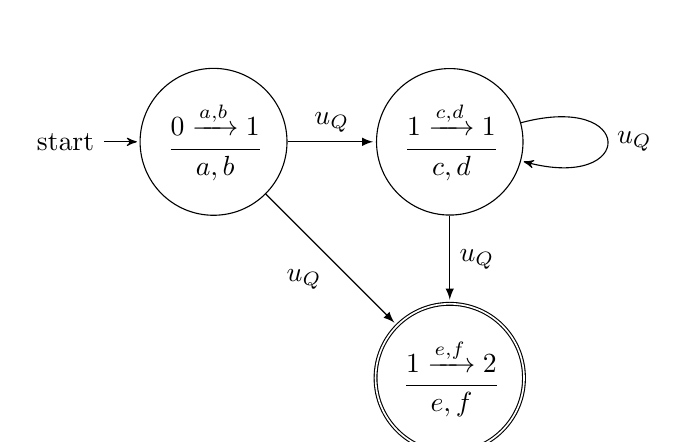
\begin{tikzpicture}[>=stealth',shorten >=1pt,node distance=2cm,on grid,auto] 
	
	%Automata states
	\node[state,initial] (q_0)   {$\cfrac{0 \xrightarrow[]{a,b} 1}{a,b}$}; 
	\node[state] (q_1) [right=3cm of q_0] {$\cfrac{1 \xrightarrow[]{c,d} 1}{c,d}$}; 
	\node[state,accepting] (q_2) [below=3cm of q_1] {$\cfrac{1 \xrightarrow[]{e,f} 2}{e,f}$}; 
	
	%Automata Paths
	\path[-latex] 
	(q_0) edge 				node 	    {$u_Q$} (q_1)
	edge				node [swap] {$u_Q$} (q_2)
	(q_1) edge 				node 		{$u_Q$} (q_2)
	edge [loop right] node 		{$u_Q$} ();
	
	\end{tikzpicture}

\end{figure}

\section{Example \theblockDiagram}
\stepcounter{blockDiagram}

\begin{figure}[h]
	\begin{center}
		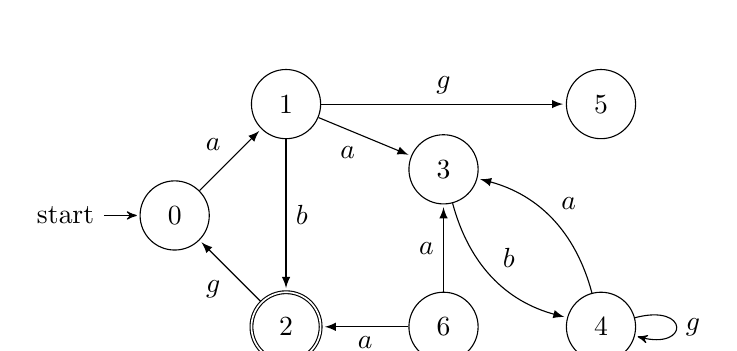
\begin{tikzpicture}[>=stealth',shorten >=1pt,node distance=2cm,on grid,auto] 
		
		%Automata states
		\node[state,initial] (q_0)   {$0$}; 
		\node[state] (q_1) [above right=of q_0] {$1$}; 
		\node[state,accepting] (q_2) [below right=of q_0] {$2$}; 
		\node[state] (q_6) [right=of q_2] {$6$};
		\node[state] (q_3) [above =of q_6] {$3$};
		\node[state] (q_4) [right=of q_6] {$4$};
		\node[state] (q_5) [right=4cm of q_1] {$5$};
		
		%Automata paths
		\path[-latex] 
		(q_0) edge 				node 		{$a$} (q_1)
		(q_1) edge 				node 		{$g$} (q_5)
		edge 				node [swap]	{$a$} (q_3)
		edge 				node 		{$b$} (q_2)
		(q_3) edge [bend right]	node 		{$b$} (q_4)
		(q_4) edge [loop right] node 		{$g$} ()
		edge [bend right] node [swap]	{$a$} (q_3)
		(q_6) edge				node 		{$a$} (q_3)
		edge 				node 		{$a$} (q_2)
		(q_2) edge 				node 		{$g$} (q_0);
		
		\end{tikzpicture}
	\end{center}

\end{figure}

\section{Example \theblockDiagram}
\stepcounter{blockDiagram}

\begin{figure}[h]
	\begin{center}
		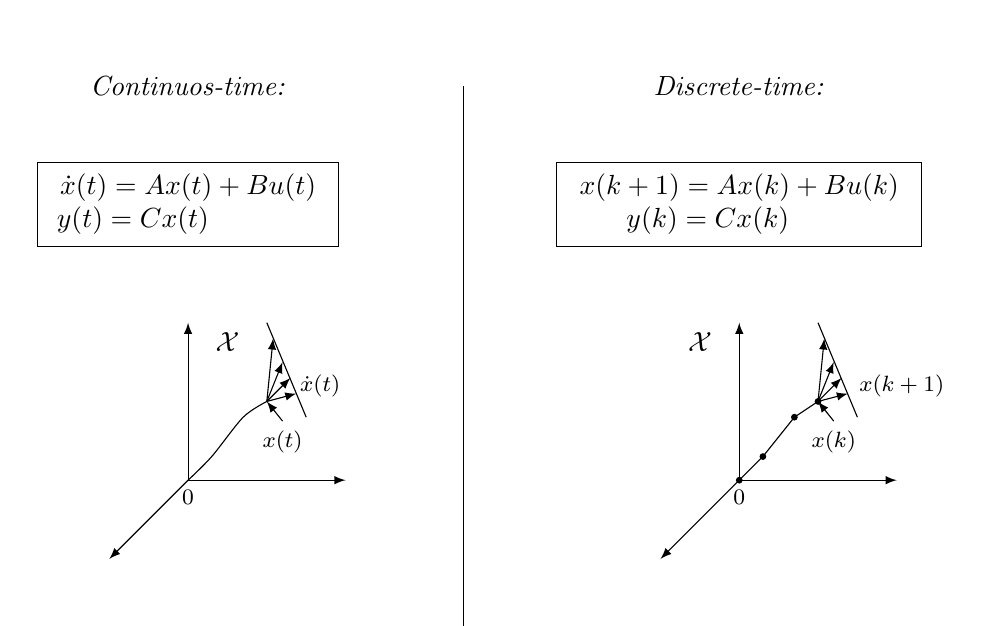
\begin{tikzpicture}
		
		%Lines separiting the two plots
		\draw[-] (0,0) coordinate -- (0,-7.0) coordinate;
		
		%Continuous-time equations
		\node (continuosTime) at (-3.5,0) [text centered]{\textit{Continuos-time:}};
		
		\node (rettangoloContinuo) at (-3.5,-1.5) []{
			
			\boxed{
				\begin{array}{cc}
				\dot{x}(t)=Ax(t)+Bu(t)\\
				\hspace{-1.4cm}y(t)=Cx(t)
				\end{array}
			}
		};
		
		%The reference system
		\draw[-latex] (-3.5,-5.0) coordinate node[below]{\footnotesize{$0$}} -- (-3.5,-3.0) 
		coordinate;
		\draw[-latex] (-3.5,-5.0) coordinate -- (-1.5,-5.0) coordinate;
		\draw[-latex] (-3.5,-5.0) coordinate -- (-4.5,-6.0) coordinate;
		
		%Smooth curve
		\draw [black] plot [smooth] coordinates {(-3.5,-5.0) (-3.2,-4.7) (-2.8,-4.2) (-2.5,-4.0)};
		
		%Line
		\draw (-2.0,-4.2) coordinate -- (-2.5,-3.0) coordinate;
		
		%Arrows
		\draw[-latex] (-2.5,-4.0) coordinate -- (-2.125,-3.9) coordinate;
		\draw[-latex] (-2.5,-4.0) coordinate -- (-2.2,-3.7) coordinate;
		\draw[-latex] (-2.5,-4.0) coordinate -- (-2.3,-3.5) coordinate;
		\draw[-latex] (-2.5,-4.0) coordinate -- (-2.42,-3.2) coordinate;
		
		%Arrows with x
		\draw[-latex] (-2.3,-4.25) coordinate node[below]{\footnotesize{$x(t)$}} -- (-2.5,-4.0) 
		coordinate;
		
		%Callygraphic X
		\draw (-3.0,-3.0) coordinate node[below]{$\mathcal{X}$};
		
		%Xdot depicting
		\draw (-2.2,-3.8) node[right]{\footnotesize{$\dot{x}(t)$}};
		
		
		%%%%%%%%%%%%%%%%%%%%%%%%%%%%%%%%%%%%%
		%Discre-time equations
		\node (discreteTime) at (3.5,0) [text centered]{\textit{Discrete-time:}};
		
		\node (rettangoloContinuo) at (3.5,-1.5) []{
			
			\boxed{
				\begin{array}{cc}
				x(k+1)=Ax(k)+Bu(k)\\
				\hspace{-0.8cm}y(k)=Cx(k)
				\end{array}
			}
		};
		
		%Reference systems
		\draw[-latex] (3.5,-5.0) coordinate node[below]{\footnotesize{$0$}} -- (3.5,-3.0) 
		coordinate;
		\draw[-latex] (3.5,-5.0) coordinate -- (5.5,-5.0) coordinate;
		\draw[-latex] (3.5,-5.0) coordinate -- (2.5,-6.0) coordinate;
		
		%Smooht curve
		\draw[black] plot coordinates {(3.5,-5.0) (3.8,-4.7) (4.2,-4.2) (4.5,-4.0)};
		\filldraw (3.5,-5.0) circle (1pt);
		\filldraw (3.8,-4.7) circle (1pt);
		\filldraw (4.2,-4.2) circle (1pt);
		\filldraw (4.5,-4.0) circle (1pt);
		
		%Line
		\draw (5.0,-4.2) coordinate -- (4.5,-3.0) coordinate;
		
		%Callygraphics x
		\draw (3.0,-3.0) coordinate node[below]{$\mathcal{X}$};
		
		%Depecting xk+a
		\draw (4.9,-3.8) node[right]{\footnotesize{$x(k+1)$}};
		
		%Arrow with x
		\draw[-latex] (4.7,-4.25) coordinate node[below]{\footnotesize{$x(k)$}} -- (4.5,-4.0) 
		coordinate;
		
		%Arrows representation
		\draw[-latex] (4.5,-4.0) coordinate -- (4.88,-3.9) coordinate;
		\draw[-latex] (4.5,-4.0) coordinate -- (4.8,-3.7) coordinate;
		\draw[-latex] (4.5,-4.0) coordinate -- (4.7,-3.5) coordinate;
		\draw[-latex] (4.5,-4.0) coordinate -- (4.58,-3.2) coordinate;
		
		\end{tikzpicture}
	\end{center}
\end{figure}


\section{Example \theblockDiagram}
\stepcounter{blockDiagram}

\begin{figure}[h]
	\begin{center}
			\begin{tikzpicture}[node distance=2cm]
			
			%Blocks
			\node (virtualReality) at (2.5,0) [rectangle, draw, text centered, minimum width=2.5cm, 
			minimum height=1cm] {Virtual Reality};
			\node (classifier) at (-2,0) [rectangle, draw, text centered, minimum width=2.5cm, 
			minimum height=1cm] {Classifier};
			\node (computing) at (-3,3)  [rectangle, draw, text centered, minimum width=2.5cm, 
			minimum height=1cm] {Computing};
			\node (controller) at (0.5,3) [rectangle, draw, text centered, minimum 
			width=2.5cm,minimum height=1cm] {Controller};
			\node (car) at (7.8,-0.25) [rectangle, draw, text centered, minimum width=2.5cm, 
			minimum height=1cm] {Car};
			\node (drone) at (4.0,3) [rectangle, draw, text centered, minimum width=2.5cm, minimum 
			height=1cm] {Drone};
			
			%Links
			\draw [-latex] (virtualReality.west) -- (classifier.east);
			\draw [-latex] (classifier.west) -- (-5.0,0) -- (-5.0,3) -- (computing.west);
			\draw [-latex] (computing.east) -- (controller.west);
			\draw [-latex] (controller.east) -- (drone.west);
			\draw [-latex] (car.west) -- (3.9,-0.25);
			\draw [-latex] (drone.east) -- (6.0,3) -- (6.0,0.255) -- (3.9,0.255);
			\draw [-latex] (5.7,3) -- (5.7,4.5) -- (0.5,4.5) -- (controller.north);
			\node (circle) at (5.7,3) [circle, draw, scale=0.4, fill=black] {};
			
			\end{tikzpicture}
	\end{center}

\end{figure}

\newpage

\section{Example \theblockDiagram}
\stepcounter{blockDiagram}

\begin{figure}[h]
	\begin{center}
		\begin{tikzpicture}
		
		%Reference system
		\draw[dashed] (0,0) coordinate -- (0,1) coordinate;
		\draw[-latex] (0,1) coordinate -- (0,3) coordinate node[above left]{$y$};
		\draw[dashed] (0,0) coordinate -- (1,0) coordinate;
		\draw[-] (1,0) coordinate -- (3,0) coordinate node[above right]{$-x$};
		\draw[dashed] (0,0) coordinate -- (-1.2,0) coordinate;
		\draw[-latex] (-1.2,0) coordinate -- (-3,0) coordinate node[above left]{$x$};
		\node (circle) at (0,0) [circle, draw, dashed, minimum size=0.5cm]{};
		\node[circle,draw,black,scale=0.3, fill=black] at (0,0) {};
		\draw (0,-0.25) coordinate node[below left]{$z$};
		
		%Camera
		\draw[-, line width=1.25pt] (1,1) coordinate -- (-1,1) coordinate;
		\draw[-, line width=1.25pt] (1,-1) coordinate -- (-1,-1) coordinate;
		\draw[-, line width=1.25pt] (1,-1) coordinate -- (1,1) coordinate;
		\draw[-, line width=1.25pt] (-1,-1) coordinate -- (-1,1) coordinate;
		
		\draw[-, line width=1.25pt] (-1,-1) coordinate -- (-1.2,-1.2) coordinate;
		\draw[-, line width=1.25pt] (-1,1) coordinate -- (-1.2,1.2) coordinate;
		\draw[-, line width=1.25pt] (-1.2,1.2) coordinate -- (-1.2,-1.2) coordinate;
		
		\end{tikzpicture}
	\end{center}
	
\end{figure}


\section{Example \theblockDiagram}
\stepcounter{blockDiagram}

\begin{figure}[h]
	\begin{center}
		\scalebox{0.8}{
			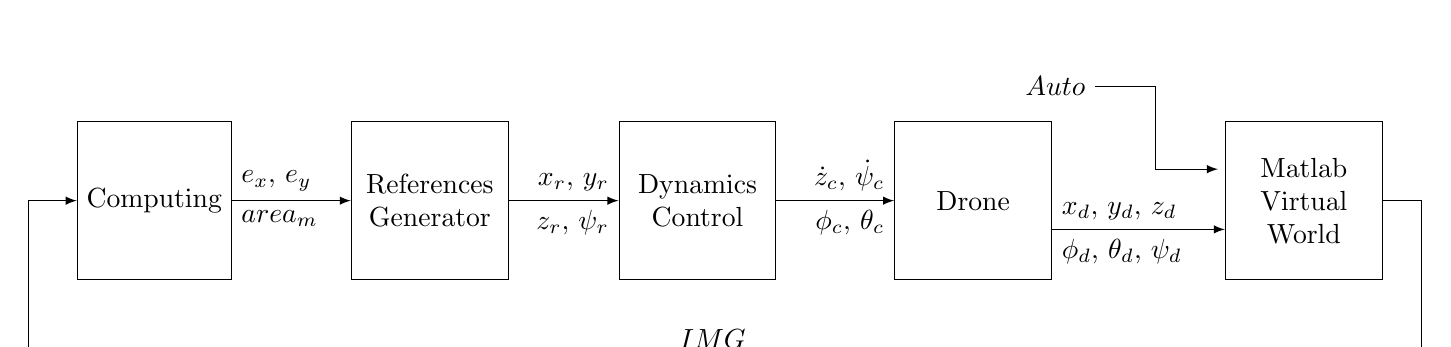
\begin{tikzpicture}
			
			%Computing block
			\node (computing) at (-4.2,0) [draw, rectangle, text centered, minimum width=1cm, 
			minimum height=2cm]{Computing};
			
			%Reference generator
			\node (referenceGenerator) at (-0.7,0) [draw, rectangle, minimum width=1cm, text 
			width=5em, minimum height=2cm, text centered]{References\\ Generator};
			
			%Trajectory controller
			\node (trajectoryController) at (2.7,0) [draw, rectangle, minimum width=1cm, minimum 
			height=2cm, text centered, text width=5em]{Dynamics\\ Control};
			
			%Drone
			\node (drone) at (6.2,0) [draw, rectangle, minimum width=1cm, minimum height=2cm, text 
			centered, text width=5em]{Drone};
			
			%Matlab virtual world
			\node (virtualWorld) at (10.4,0) [draw, rectangle, minimum width=1cm, minimum 
			height=2cm, text centered, text width=5em]{Matlab \\Virtual World};
			
			%Links among blocks
			\draw[-latex] (computing.east) node[above right]{$e_x,\,e_y$} node[below 
			right]{$area_m$}-- (referenceGenerator.west);
			\draw[-latex] (referenceGenerator.east) -- (trajectoryController.west) node[below 
			left]{$z_r,\,\psi_r$} node[above left]{$x_r,\,y_r$};
			\draw[-latex] (trajectoryController.east) -- (drone.west) node[above 
			left]{$\dot{z}_c,\,\dot{\psi}_c$} node[below left]{$\phi_c,\,\theta_c$};
			\draw[-latex] (drone.-20) node[below right]{$\phi_d,\,\theta_d,\,\psi_d$} node[above 
			right]{$x_d,\,y_d,\,z_d$} -- (virtualWorld.200);
			\draw[-latex] (virtualWorld.east) -- (11.9,0) coordinate -- (11.9,-2.0) coordinate 
			--(-5.8,-2.0) coordinate -- (-5.8,0) coordinate -- (computing.west);
			\draw (2.35,-2.0) coordinate node[above right]{$IMG$};
			
			%Link for connecting the car block
			\draw[-latex] (7.75,1.45) coordinate node[left]{$Auto$}-- (8.52,1.45) coordinate -- 
			(8.52,0.4) coordinate -- (9.31,0.4) coordinate;
			
			\end{tikzpicture}
		}
	\end{center}
	
\end{figure}


\section{Example \theblockDiagram}
\stepcounter{blockDiagram}

\begin{figure}[h]
	\begin{center}
		\scalebox{0.7}{
			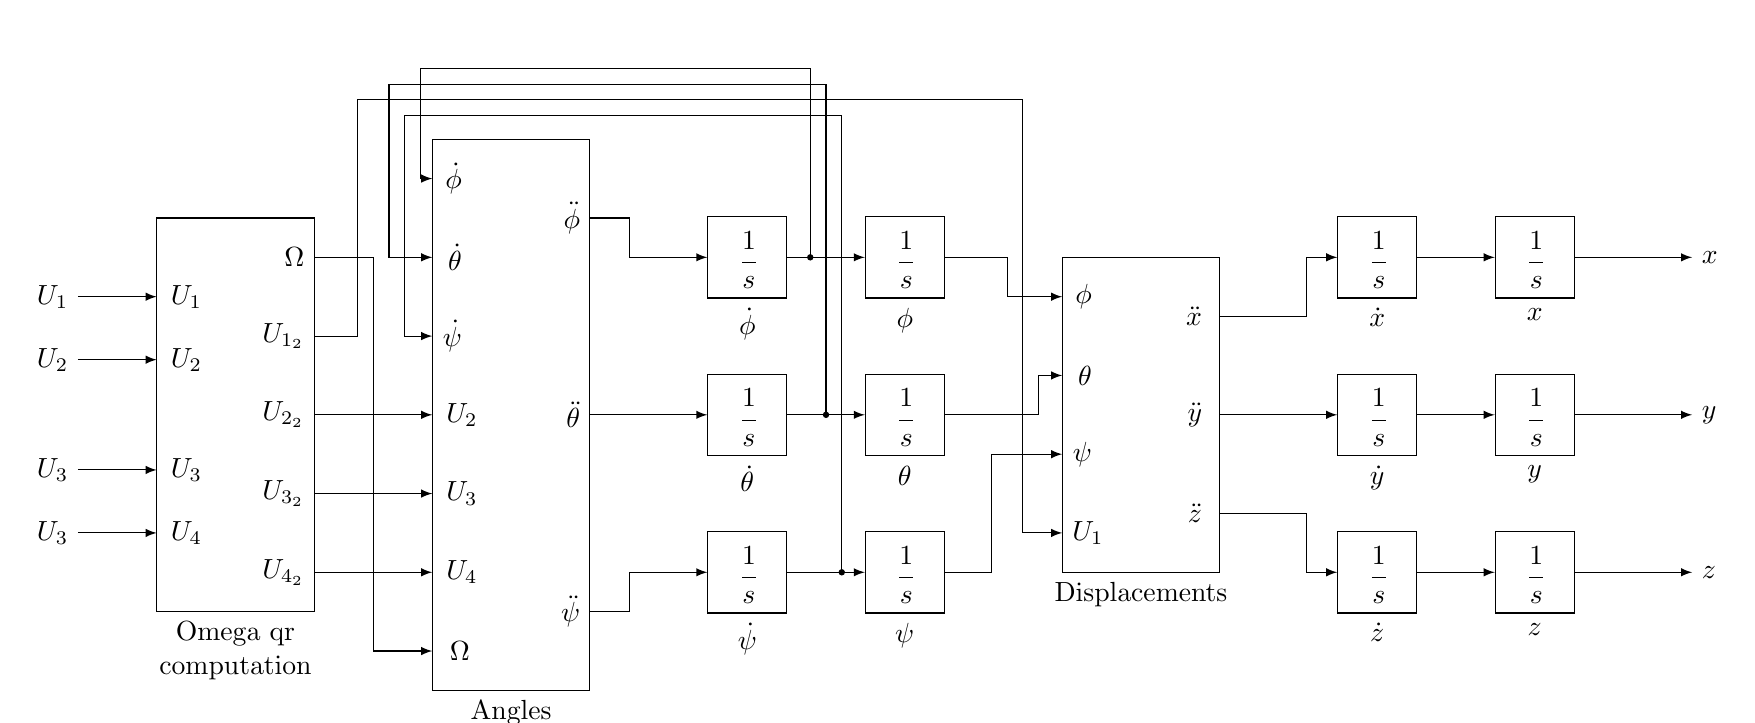
\begin{tikzpicture}
			
			%Initial links
			\draw[-latex] (-5.5,1.5) coordinate node[left]{$U_1$} -- (-4.5,1.5) coordinate;
			\draw[-latex] (-5.5,0.7) coordinate node[left]{$U_2$} -- (-4.5,0.7) coordinate;
			\draw[-latex] (-5.5,-0.7) coordinate node[left]{$U_3$} -- (-4.5,-0.7) coordinate;
			\draw[-latex] (-5.5,-1.5) coordinate node[left]{$U_3$} -- (-4.5,-1.5) coordinate;
			
			%Omega qr calculator block
			\node (omegaQRCalculator) at (-3.5,0) [draw, rectangle, minimum height=5cm, minimum 
			width=2cm, text centered, label={[align=center]below:Omega qr\\computation}]{};
			
			%Variables - omega qr calculator
			\draw (-3.8, 1.5) coordinate node[left]{$U_{1}$};
			\draw (-3.8, 0.7) coordinate node[left]{$U_{2}$};
			\draw (-3.8, -0.7) coordinate node[left]{$U_{3}$};
			\draw (-3.8, -1.5) coordinate node[left]{$U_{4}$};
			
			\draw (-2.5, 2.0) coordinate node[left]{$\Omega$};
			\draw (-2.5, 1.0) coordinate node[left]{$U_{1_{2}}$};
			\draw (-2.5, 0.0) coordinate node[left]{$U_{2_{2}}$};
			\draw (-2.5, -1.0) coordinate node[left]{$U_{3_{2}}$};
			\draw (-2.5, -2.0) coordinate node[left]{$U_{4_{2}}$};
			
			%Links between the omega and angles blocks
			\draw[-latex] (-2.5,2.0) coordinate -- (-1.75,2.0) coordinate -- (-1.75,-3.0) 
			coordinate -- (-1,-3.0) coordinate;
			\draw[-latex] (-2.5,1.0) coordinate -- (-1.95,1.0) coordinate -- (-1.95,4.0) coordinate 
			-- (6.5,4.0) coordinate -- (6.5,-1.5) coordinate -- (7,-1.5) coordinate;
			\draw[-latex] (-2.5,0.0) coordinate -- (-1,0.0) coordinate;
			\draw[-latex] (-2.5,-1.0) coordinate -- (-1,-1.0) coordinate;
			\draw[-latex] (-2.5,-2.0) coordinate -- (-1,-2.0) coordinate;
			
			%Angles block
			\node (anglesBlock) at (0,0) [draw, rectangle, minimum height=7cm, minimum width=2cm, 
			text centered, label={[align=center]below:Angles}]{};
			
			%Variables - angles
			\draw (-0.5,3.0) coordinate node[left]{$\dot{\phi}$};
			\draw (-0.5,2.0) coordinate node[left]{$\dot{\theta}$};
			\draw (-0.5,1.0) coordinate node[left]{$\dot{\psi}$};
			\draw (-0.3,0.0) coordinate node[left]{$U_2$};
			\draw (-0.3,-1.0) coordinate node[left]{$U_3$};
			\draw (-0.3,-2.0) coordinate node[left]{$U_4$};
			\draw (-0.4,-3.0) coordinate node[left]{$\Omega$};
			
			\draw (1.0, 2.5) coordinate node[left]{$\ddot{\phi}$};
			\draw (1.0, 0.0) coordinate node[left]{$\ddot{\theta}$};
			\draw (1.0, -2.5) coordinate node[left]{$\ddot{\psi}$};
			
			%First integrator block - angles
			\node (integrator1) at (3,0) [draw, rectangle, minimum height=1cm, minimum width=1cm, 
			text centered, label={[align=center]below:$\dot{\theta}$}]{$\cfrac{1}{s}$};
			\node (integrator2) at (3,2) [draw, rectangle, minimum height=1cm, minimum width=1cm, 
			text centered, label={[align=center]below:$\dot{\phi}$}]{$\cfrac{1}{s}$};
			\node (integrator3) at (3,-2) [draw, rectangle, minimum height=1cm, minimum width=1cm, 
			text centered, label={[align=center]below:$\dot{\psi}$}]{$\cfrac{1}{s}$};
			
			%Links between the angles and integrator blocks
			\draw[-latex] (1.0,2.5) coordinate -- (1.5,2.5) coordinate -- (1.5,2.0) coordinate -- 
			(integrator2.west);
			\draw[-latex] (1.0,0.0) coordinate -- (integrator1.west);
			\draw[-latex] (1.0,-2.5) coordinate -- (1.5,-2.5) coordinate -- (1.5,-2.0) coordinate 
			-- (integrator3.west);
			
			%Second integrators block - angles
			\node (integrator4) at (5,0) [draw, rectangle, minimum height=1cm, minimum width=1cm, 
			text centered, label={[align=center]below:$\theta$}]{$\cfrac{1}{s}$};
			\node (integrator5) at (5,2) [draw, rectangle, minimum height=1cm, minimum width=1cm, 
			text centered, label={[align=center]below:$\phi$}]{$\cfrac{1}{s}$};
			\node (integrator6) at (5,-2) [draw, rectangle, minimum height=1cm, minimum width=1cm, 
			text centered, label={[align=center]below:$\psi$}]{$\cfrac{1}{s}$};
			
			%Circle on the connection links
			\node[circle,draw,black,scale=0.2, fill=black] (A) at (4,0){};
			\node[circle,draw,black,scale=0.2, fill=black] (A) at (4.2,-2){};
			\node[circle,draw,black,scale=0.2, fill=black] (A) at (3.8,2){};
			
			%Links among blocks
			\draw[-latex] (4,0) coordinate -- (4,4.2) coordinate -- (-1.55,4.2) coordinate -- 
			(-1.55,2.0) coordinate -- (-1.0,2.0);
			\draw[-latex] (4.2,-2) coordinate -- (4.2,3.8) coordinate -- (-1.35,3.8) coordinate -- 
			(-1.35,1.0) coordinate -- (-1.0,1.0);
			\draw[-latex] (3.8,2) coordinate -- (3.8,4.4) coordinate -- (-1.15,4.4) coordinate -- 
			(-1.15,3.0) coordinate -- (-1.0,3.0);
			
			%Links among integrators blocks
			\draw[-latex] (integrator1.east) -- (integrator4.west);
			\draw[-latex] (integrator2.east) -- (integrator5.west);
			\draw[-latex] (integrator3.east) -- (integrator6.west);
			
			%Connection links between the integrators and displacement blocks
			\draw[-latex] (integrator5.east) -- (6.3,2) coordinate -- (6.3,1.5) coordinate -- 
			(7.0,1.5) coordinate;
			\draw[-latex] (integrator4.east) -- (6.7,0.0) coordinate -- (6.7,0.5) coordinate -- 
			(7.0,0.5) coordinate;
			\draw[-latex] (integrator6.east) -- (6.1,-2) coordinate -- (6.1,-0.5) coordinate -- 
			(7.0,-0.5) coordinate;
			
			%Displacement block
			\node (bloccoDisplacement) at (8,0) [draw, rectangle, minimum height=4cm, minimum 
			width=2cm, text centered, label={[align=center]below:Displacements}]{};
			
			%Variables - displacement
			\draw (7.5,1.5) coordinate node[left]{$\phi$};
			\draw (7.5,0.5) coordinate node[left]{$\theta$};
			\draw (7.5,-0.5) coordinate node[left]{$\psi$};
			\draw (7.65,-1.5) coordinate node[left]{$U_1$};
			
			\draw (8.9,1.25) coordinate node[left]{$\ddot{x}$};
			\draw (8.9,0.0) coordinate node[left]{$\ddot{y}$};
			\draw (8.9,-1.25) coordinate node[left]{$\ddot{z}$};
			
			%First integrators block - displacement
			\node (integrator7) at (11,0) [draw, rectangle, minimum height=1cm, minimum width=1cm, 
			text centered, label={[align=center]below:$\dot{y}$}]{$\cfrac{1}{s}$};
			\node (integrator8) at (11,2) [draw, rectangle, minimum height=1cm, minimum width=1cm, 
			text centered, label={[align=center]below:$\dot{x}$}]{$\cfrac{1}{s}$};
			\node (integrator9) at (11,-2) [draw, rectangle, minimum height=1cm, minimum width=1cm, 
			text centered, label={[align=center]below:$\dot{z}$}]{$\cfrac{1}{s}$};
			
			%Links for the displacement block
			\draw[-latex] (9,1.25) coordinate -- (10.1,1.25) coordinate -- (10.1,2) coordinate -- 
			(integrator8.west);
			\draw[-latex] (9,0.0) coordinate -- (integrator7.west);
			\draw[-latex] (9,-1.25) coordinate -- (10.1,-1.25) coordinate -- (10.1,-2) coordinate 
			-- (integrator9.west);
			
			%Second block of integrators - displacement
			\node (integrator10) at (13,0) [draw, rectangle, minimum height=1cm, minimum width=1cm, 
			text centered,label={[align=center]below:$y$}]{$\cfrac{1}{s}$};
			\node (integrator11) at (13,2) [draw, rectangle, minimum height=1cm, minimum width=1cm, 
			text centered,label={[align=center]below:$x$}]{$\cfrac{1}{s}$};
			\node (integrator12) at (13,-2) [draw, rectangle, minimum height=1cm, minimum 
			width=1cm, text centered,label={[align=center]below:$z$}]{$\cfrac{1}{s}$};
			
			%Connections between the two integrators blocks
			\draw[-latex] (integrator7.east) -- (integrator10.west);
			\draw[-latex] (integrator8.east) -- (integrator11.west);
			\draw[-latex] (integrator9.east) -- (integrator12.west);
			
			%Final interconnections
			\draw[-latex] (integrator10.east) -- (15,0) coordinate node[right]{$y$};
			\draw[-latex] (integrator11.east) -- (15,2) coordinate node[right]{$x$};
			\draw[-latex] (integrator12.east) -- (15,-2) coordinate node[right]{$z$};
			
			\end{tikzpicture}
		}
	\end{center}
	
\end{figure}

\section{Example \theblockDiagram}
\stepcounter{blockDiagram}

\begin{figure}[h]
	\begin{center}
		\scalebox{0.85}{
			
			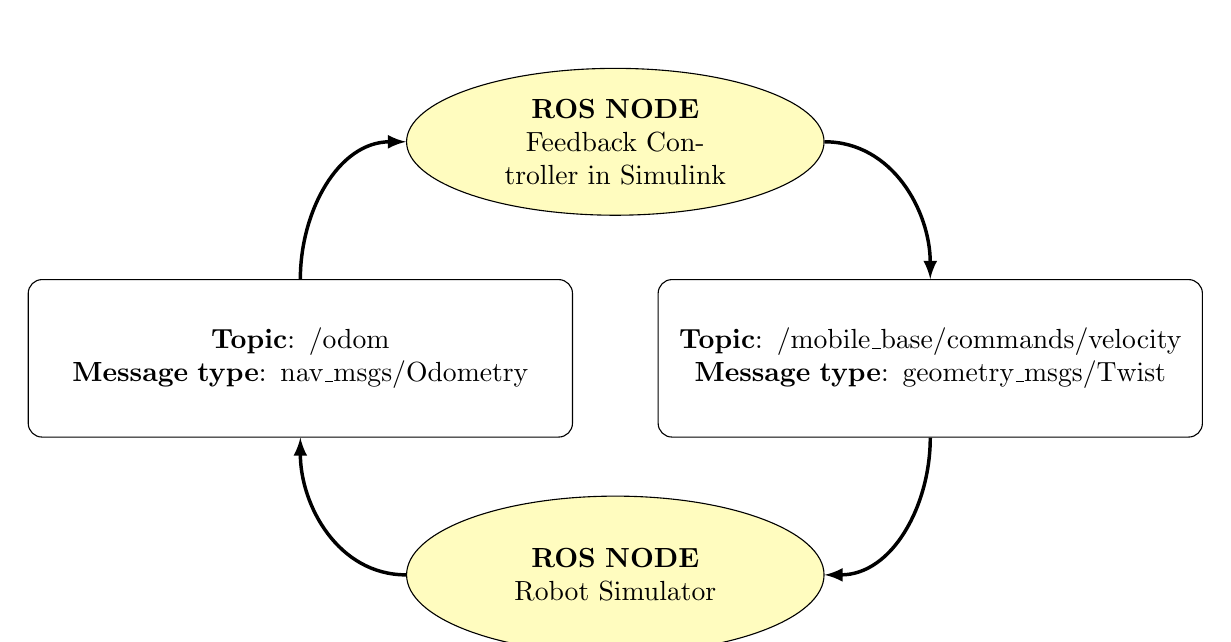
\begin{tikzpicture}
			\node (feedbackController) at (0,1.25) [draw, ellipse, text centered, minimum 
			height=1cm, fill=yellow!25, text width=10em]{\textbf{ROS NODE}\\Feedback Controller in 
			Simulink};
			\node (robotSimulator) at (0,-4.25) [draw, ellipse, text centered, minimum 
			height=2cm,fill=yellow!25, text width=10em]{\textbf{ROS NODE}\\Robot Simulator};
			
			\node (odom) at (-4,-1.5) [draw, rectangle, text centered, text width=19em, minimum 
			height=2cm, rounded corners=5pt]{\textbf{Topic}: /odom\\\textbf{Message type}: 
			nav\_msgs/Odometry};
			\node (mobileBase) at (4,-1.5) [draw, rectangle, text centered, text width=19em, 
			minimum height=2cm, rounded corners=5pt]{\textbf{Topic}: 
			/mobile\_base/commands/velocity\\\textbf{Message type}: geometry\_msgs/Twist};
			
			\draw[-latex, line width=1.25pt] (feedbackController) [out=0, in=90] to (mobileBase);
			\draw[-latex, line width=1.25pt] (mobileBase) [out=270, in=0] to (robotSimulator);
			\draw[-latex, line width=1.25pt] (robotSimulator) [out=180, in=270] to (odom);
			\draw[-latex, line width=1.25pt] (odom) [out=90, in=180] to (feedbackController); 
			
			\end{tikzpicture}
		}
	\end{center}
\end{figure}


\section{Example \theblockDiagram}
\stepcounter{blockDiagram}

\begin{figure}[h]
	\begin{center}
		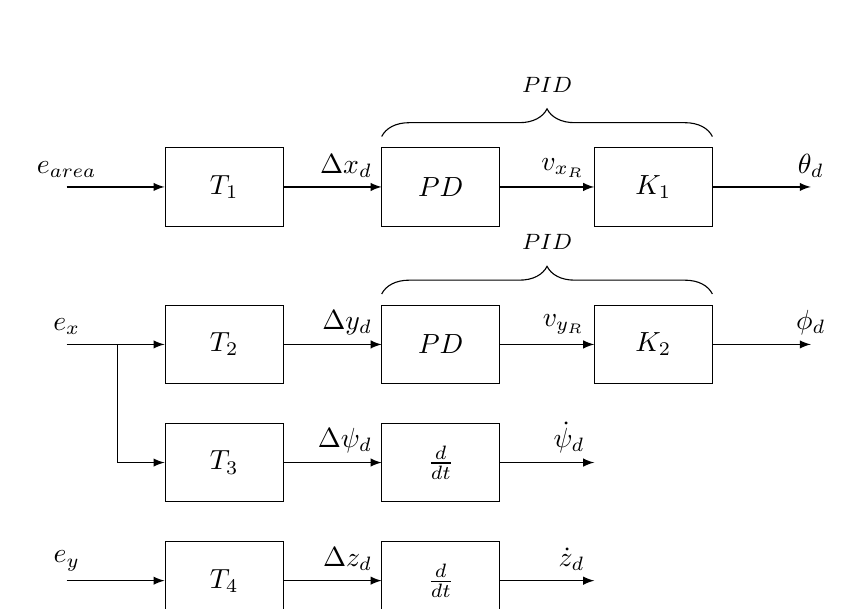
\begin{tikzpicture}
		
		%Nodes in the first part of the scheme
		\node (firstTransformation) at (-2,0.5) [draw, rectangle, minimum width=1.5cm, minimum 
		height=1cm, text centered]{$T_1$};
		
		\node (firstPD) at (0.75,0.5) [draw, text centered, minimum width=1.5cm, minimum 
		height=1cm]{$PD$};
		
		\node (firstK) at (3.45,0.5) [draw, text centered, minimum width=1.5cm, minimum 
		height=1cm]{$K_1$};
		
		\draw [decorate,decoration={brace, mirror, amplitude=10pt,raise=4pt},yshift=0pt]
		(4.2,1) -- (0,1) node [black,midway,yshift=0.8cm] {\footnotesize $PID$};
		
		%Links
		\draw[-latex] (-4,0.5) coordinate node[above]{$e_{area}$} -- (firstTransformation.west);
		
		\draw[-latex] (firstTransformation.east) -- (0,0.5) coordinate node[above left]{$\Delta 
		x_d$};
		
		\draw[-latex] (firstPD.east) -- (2.7,0.5) coordinate node[above left]{$v_{{x}_R}$};
		
		\draw[-latex] (firstK.east) -- (5.45,0.5) coordinate node[above]{$\theta_d$};
		
		
		%Nodes in the second part of the scheme
		\node (secondTransformation) at (-2,-1.5) [draw, rectangle, minimum width=1.5cm, minimum 
		height=1cm, text centered]{$T_2$};
		
		\node (secondPD) at (0.75,-1.5) [draw, text centered, minimum width=1.5cm, minimum 
		height=1cm]{$PD$};
		
		\node (secondK) at (3.45,-1.5) [draw, text centered, minimum width=1.5cm, minimum 
		height=1cm]{$K_2$};
		
		\draw [decorate,decoration={brace, mirror, amplitude=10pt,raise=4pt},yshift=0pt]
		(4.2,-1.0) -- (0,-1.0) node [black,midway,yshift=0.8cm] {\footnotesize
			$PID$};
		
		%Links among blocks
		\draw[-latex] (-4,-1.5) coordinate node[above]{$e_x$} -- (secondTransformation.west);
		
		\draw[-latex] (secondTransformation.east) -- (0,-1.5) coordinate node[above left]{$\Delta 
		y_d$};
		
		\draw[-latex] (secondPD.east) -- (2.7,-1.5) coordinate node[above left]{$v_{{y}_R}$};
		
		\draw[-latex] (secondK.east) -- (5.45,-1.5) coordinate node[above]{$\phi_d$};
		
		
		%Nodes in the third part of the scheme
		\node (thirdTransformation) at (-2,-3.0) [draw, rectangle, minimum width=1.5cm, minimum 
		height=1cm, text centered]{$T_3$};
		
		\node (thirdPD) at (0.75,-3.0) [draw, text centered, minimum width=1.5cm, minimum 
		height=1cm]{$\frac{d}{dt}$};
		
		%Links among blocks
		\draw[-latex] (-3.35, -1.5) coordinate --  (-3.35,-3.0) coordinate -- 
		(thirdTransformation.west);
		
		\draw[-latex] (thirdTransformation.east) -- (0,-3.0) coordinate node[above left]{$\Delta 
		\psi_d$};
		
		\draw[-latex] (thirdPD.east) -- (2.7,-3.0) coordinate node[above left]{$\dot{\psi}_d$};
		
		
		%Nodes of the fourth part of the scheme
		\node (fourthTransformation) at (-2,-4.5) [draw, rectangle, minimum width=1.5cm, minimum 
		height=1cm, text centered]{$T_4$};
		
		\node (fourthPD) at (0.75,-4.5) [draw, text centered, minimum width=1.5cm, minimum 
		height=1cm]{$\frac{d}{dt}$};
		
		%Links among blocks
		\draw[-latex] (-4,-4.5) coordinate node[above]{$e_y$} -- (fourthTransformation.west);
		
		\draw[-latex] (fourthTransformation.east) -- (0,-4.5) coordinate node[above left]{$\Delta 
		z_d$};
		
		\draw[-latex] (fourthPD.east) -- (2.7,-4.5) coordinate node[above left]{$\dot{z}_d$};
		
		
		\end{tikzpicture}
	\end{center}
	
\end{figure}

\newpage

\section{Example \theblockDiagram}
\stepcounter{blockDiagram}

\begin{figure}[h]
	\begin{center}
		\scalebox{1}{
			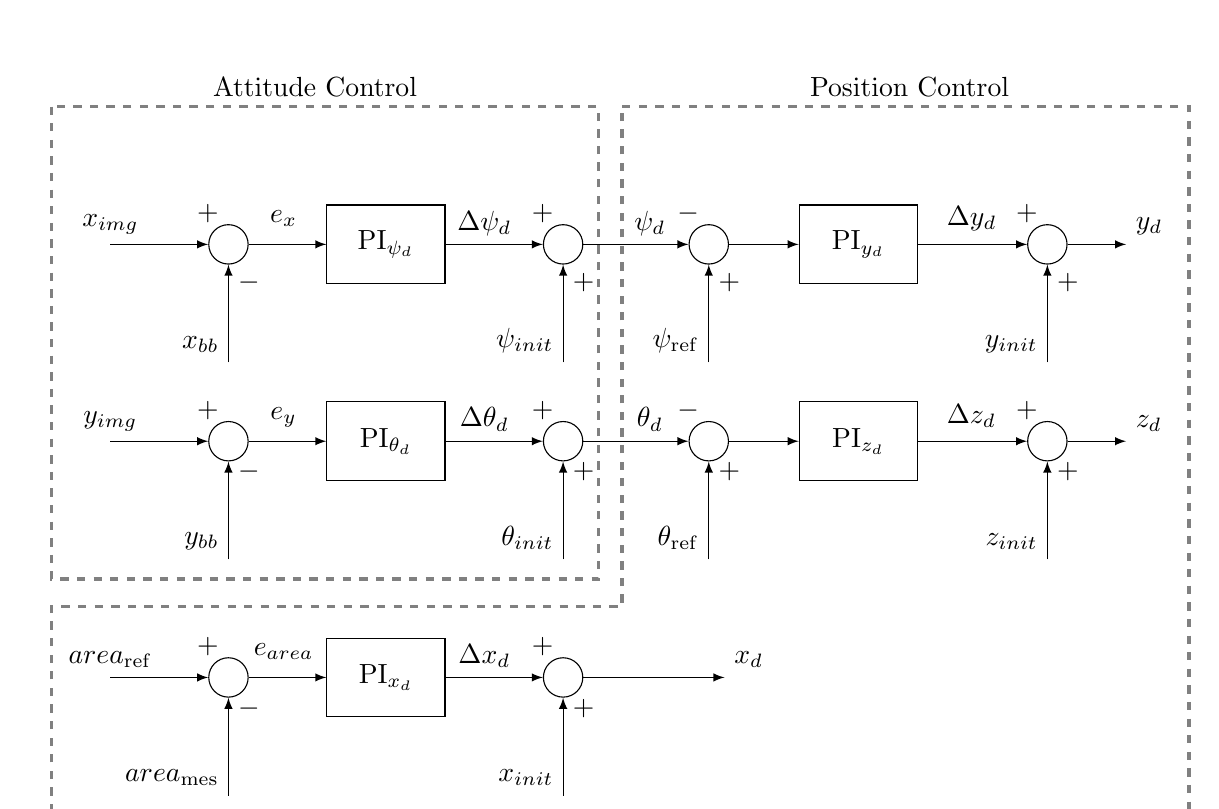
\begin{tikzpicture}
			
			%Attitude controller
			\node (attitudeController) at (-3.40,-1.25) [rectangle, label=Attitude Control, text 
			centered, minimum height=6cm, minimum width=7.3cm]{};
			
			\draw[dashed, gray, line width=1.25pt] (-6.75,1.75) coordinate -- (-6.75,-4.25) 
			coordinate -- (0.2,-4.25) coordinate -- (0.2,1.75) coordinate -- (-6.75,1.75) 
			coordinate;
			
			%Position controller
			\draw[dashed, gray, line width=1.25pt] (0.5, 1.75) coordinate -- (7.7, 1.75) coordinate 
			-- (7.7, -7.3) coordinate --  (-6.75,-7.3) coordinate -- (-6.75,-4.6) coordinate --  
			(0.5,-4.6) coordinate -- (0.5,1.75) coordinate;
			
			\node (positionController) at (4.15,-1.25) [label=Position Control, text centered, 
			minimum width=2.65cm, minimum height=6cm, rectangle]{};
			
			%Blocks in the first part of the scheme
			\node (adder1) at (-4.5,0) [draw, circle, text centered, minimum size=0.5cm]{};
			
			\node (pi1) at (-2.5,0) [draw, rectangle, text centered, minimum height=1.0cm, minimum 
			width=1.5cm]{$\text{PI}_{\psi_d}$};
			
			\node (adder2) at (-0.25,0) [draw, circle, text centered, minimum size=0.5cm]{};
			
			\node (adder20) at (1.6,0) [draw, circle, text centered, minimum size=0.5cm]{};
			
			\node (pi2) at (3.5,0) [draw, rectangle, text centered, minimum height=1cm, minimum 
			width=1.5cm]{$\text{PI}_{y_d}$};
			
			\node (adder6) at (5.9,0) [draw, circle, text centered, minimum size=0.5cm]{};
			
			%Links among blocks
			\draw[-latex] (-6.0,0) coordinate node[above]{$x_{img}$} -- (adder1.west);
			\draw[-latex] (-4.5,-1.5) coordinate node[above left]{$x_{bb}$} -- (adder1.south);
			
			\draw[-latex] (adder1.east) -- (pi1.west);
			\draw[-latex] (pi1.east) -- (adder2.west);
			
			\draw[-latex] (-0.25,-1.5) coordinate node[above left]{$\psi_{init}$}-- (adder2.south);
			
			\draw[-latex] (1.6,-1.5) coordinate node[above left]{$\psi_\mathrm{ref}$} -- 
			(adder20.south);
			
			\draw[-latex] (adder2.east) -- (adder20.west);
			\draw[-latex] (adder20.east) -- (pi2.west);
			\draw[-latex] (pi2.east) -- (adder6.west);
			\draw (4.5,0.05) node[above right]{$\Delta y_d$};
			
			\draw[-latex] (5.9,-1.5) coordinate node[above left]{$y_{init}$} -- (adder6.south);
			\draw[-latex] (adder6.east) -- (6.9,0) coordinate node[above right]{$y_d$};
			
			%Signs
			\draw (-4.5,0.15) coordinate node[above left]{$+$};
			\draw (-4.5,-0.25) coordinate node[below right]{$-$};
			
			\draw (-0.25,0.15) coordinate node[above left]{$+$};
			\draw (-0.25,-0.25) coordinate node[below right]{$+$};
			
			\draw (1.6,0.15) coordinate node[above left]{$-$};
			\draw (1.6,-0.25) coordinate node[below right]{$+$};
			
			\draw (5.9,0.15) coordinate node[above left]{$+$};
			\draw (5.9,-0.25) coordinate node[below right]{$+$};
			
			%Errors
			\draw (-3.8,0.55) coordinate node[below]{$e_x$};
			\draw (-1.25,0.55) coordinate node[below]{$\Delta \psi_d$};
			\draw (0.85,0.55) coordinate node[below]{$\psi_d$};
			
			
			%Blocks in the second part of the scheme
			\node (adder3) at (-4.5,-2.5) [draw, circle, text centered, minimum size=0.5cm]{};
			
			\node (pi3) at (-2.5,-2.5) [draw, rectangle, text centered, minimum height=1.0cm, 
			minimum width=1.5cm]{$\text{PI}_{\theta_d}$};
			
			\node (adder4) at (-0.25,-2.5) [draw, circle, text centered, minimum size=0.5cm]{};
			
			\node (adder50) at (1.6,-2.5) [draw, circle, text centered, minimum size=0.5cm]{};
			
			\node (pi4) at (3.5,-2.5) [draw, rectangle, text centered, minimum height=1cm, minimum 
			width=1.5cm]{$\text{PI}_{z_d}$};
			
			\node (adder7) at (5.9,-2.5) [draw, circle, text centered, minimum size=0.5cm]{}; 
			
			%Links among blocks
			\draw[-latex] (-6.0,-2.5) coordinate node[above]{$y_{img}$} -- (adder3.west);
			\draw[-latex] (-4.5,-4.0) coordinate node[above left]{$y_{bb}$} -- (adder3.south);
			
			\draw[-latex] (adder3.east) -- (pi3.west);
			\draw[-latex] (pi3.east) -- (adder4.west);
			
			\draw[-latex] (-0.25,-4.0) coordinate node[above left]{$\theta_{init}$} -- 
			(adder4.south);
			
			\draw[-latex] (1.6,-4.0) coordinate node[above left]{$\theta_\mathrm{ref}$} -- 
			(adder50.south);
			
			\draw[-latex] (adder4.east) -- (adder50.west);
			\draw[-latex] (adder50.east) -- (pi4.west);
			\draw[-latex] (pi4.east) -- (adder7.west); 
			\draw (4.5,-2.45) coordinate node[above right]{$\Delta z_d$};
			
			\draw[-latex] (5.9,-4.0) node[above left]{$z_{init}$} -- (adder7.south);
			
			\draw[-latex] (adder7.east) -- (6.9,-2.5) coordinate node[above right]{$z_d$};
			
			%Sings
			\draw (-4.5,-2.35) coordinate node[above left]{$+$};
			\draw (-4.5,-2.65) coordinate node[below right]{$-$};
			
			\draw (-0.25,-2.35) coordinate node[above left]{$+$};
			\draw (-0.25,-2.65) coordinate node[below right]{$+$};
			
			\draw (1.6,-2.35) coordinate node[above left]{$-$};
			\draw (1.6,-2.65) coordinate node[below right]{$+$};
			
			\draw (5.9,-2.35) coordinate node[above left]{$+$};
			\draw (5.9,-2.65) coordinate node[below right]{$+$};
			
			%Errors
			\draw (-3.8,-1.95) coordinate node[below]{$e_y$};
			\draw (-1.25,-1.95) coordinate node[below]{$\Delta \theta_d$};
			\draw (0.85,-1.95) coordinate node[below]{$\theta_d$};
			
			%Blocks in the third part of the scheme
			\node (adder5) at (-4.5,-5.5) [draw, circle, text centered, minimum size=0.5cm]{};
			
			\node (pi5) at (-2.5,-5.5) [draw, rectangle, text centered, minimum height=1.0cm, 
			minimum width=1.5cm]{$\text{PI}_{x_d}$};
			
			\node (adder8) at (-0.25,-5.5) [draw, circle, text centered, minimum size=0.5cm]{};
			
			%Links
			\draw[-latex] (-6.0,-5.5) coordinate node[above]{$area_{\mathrm{ref}}$} -- 
			(adder5.west);
			\draw[-latex] (-4.5,-7.0) coordinate node[above left]{$area_{\mathrm{mes}}$} -- 
			(adder5.south);
			
			\draw[-latex] (adder5.east) -- (pi5.west);
			
			\draw[-latex] (pi5.east) -- (adder8.west);
			\draw (-1.25,-5.5) coordinate node[above]{$\Delta x_d$};
			
			\draw[-latex] (-0.25,-7.0) coordinate node[above left]{$x_{init}$} -- (adder8.south);
			
			%Signs
			\draw (-4.5,-5.35) coordinate node[above left]{$+$};
			\draw (-4.5,-5.65) coordinate node[below right]{$-$};
			
			\draw (-0.25,-5.35) coordinate node[above left]{$+$};
			\draw (-0.25,-5.65) coordinate node[below right]{$+$};
			
			\draw[-latex] (adder8.east) -- (1.8,-5.5) coordinate node[above right]{$x_d$};
			
			%Errors
			\draw (-3.8,-4.95) coordinate node[below]{$e_{area}$};
			
			
			\end{tikzpicture}
		}
	\end{center}

\end{figure}

\section{Example \theblockDiagram}
\stepcounter{blockDiagram}

\begin{figure}[h]
	\begin{center}
		\scalebox{1}{
			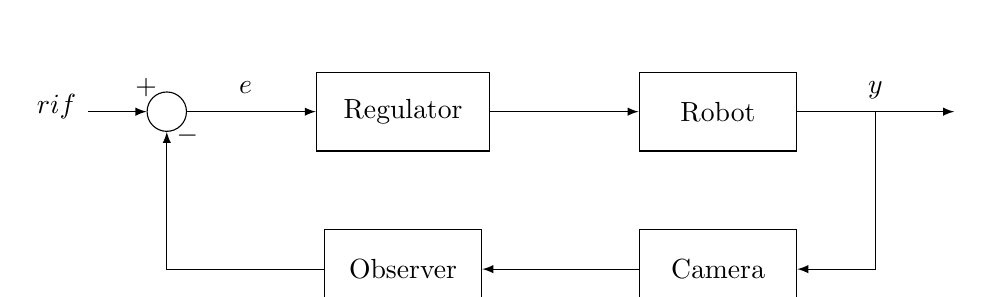
\begin{tikzpicture}[node distance=2cm]
			
			%Nodes
			\node (adder) at (0,0) [draw, circle, text centered, minimum size=0.5cm]{};
			
			\node (regulator) at (3,0) [draw, rectangle, text centered, minimum width=2.2cm, 
			minimum height=1cm]{Regulator};
			
			\node (robot) at (7,0) [draw, rectangle, text centered, minimum width=2cm, minimum 
			height=1cm]{Robot};
			
			\node (camera) at (7,-2) [draw, rectangle, text centered, minimum width=2cm, minimum 
			height=1cm]{Camera};
			
			\node (observer) at (3,-2) [draw, rectangle, text centered, minimum width=2cm, minimum 
			height=1cm]{Observer};
			
			%Links
			\draw[-latex] (adder) --  (regulator);
			\draw[-latex] (camera) -- (observer);
			\draw[-latex] (regulator) -- (robot);
			\draw[-latex] (observer.west) -- (0,-2) coordinate -- (adder.south);
			\draw[-latex] (robot.east) -- (10,0) coordinate;
			\draw[-latex] (9,0) coordinate -- (9,-2) coordinate -- (camera.east);
			\draw[-latex] (-1,0) coordinate -- (adder.west);
			
			%Variables
			\draw (9, 0.5) coordinate node[below]{$y$};
			\draw (1, 0.5) coordinate node[below]{$e$};
			\draw (-1.4,0.35) coordinate node[below]{$rif$};
			\draw (0,0.55) coordinate node[below left]{$+$};
			\draw (0,-0.55) coordinate node[above right]{$-$};
			
			\end{tikzpicture}
		}
	\end{center}
\end{figure}

\newpage


\section{Example \theblockDiagram}
\stepcounter{blockDiagram}

\begin{figure}[h]
	\begin{center}
		\scalebox{0.72}{
			\begin{tikzpicture}
			
			%Yaw angle
			\node (yawAngle) at (0,0) [draw, rectangle, minimum height=2cm, minimum width=2cm, text 
			centered]{};
			\draw (1,1) coordinate -- (1.2,1.2) coordinate;
			\draw (1,-1) coordinate -- (1.2,-1.2) coordinate;
			\draw (1.2,-1.2) coordinate -- (1.2,1.2) coordinate;
			
			%Drawing the angle
			\draw (1.8,0) coordinate -- (2.2,0) coordinate;
			\draw[-latex, line width=1.0pt] (2.0,0) coordinate -- (2.0, -1) coordinate node[above 
			right]{$\psi_d$};
			
			%Reference system
			\draw[-latex] (-4,2) coordinate -- (-4,-1) coordinate node[above left]{$z$};
			\draw[-latex] (-4,2) coordinate -- (-2,2) coordinate node[above]{$x$};
			\node (circle) at (-4,2) [circle, draw, minimum size=0.5cm]{};
			\node[circle,draw,black,scale=0.2, fill=black] (A) at (-4,2) {};
			\draw (-4.25,2) coordinate node[above left]{$y$};
			
			%Dividing line among schems
			\draw[dashed, draw=gray] (-6,-2) coordinate -- (6,-2) coordinate;
			
			%Roll angle
			\node (rollAngle) at (0,-5) [draw, rectangle, minimum height=2cm, minimum width=2cm, 
			text centered]{};
			\draw (1,-4) coordinate -- (1.2,-3.8) coordinate;
			\draw (1,-6) coordinate -- (1.2,-6.2) coordinate;
			\draw (1.2,-3.8) coordinate -- (1.2,-6.2) coordinate;
			
			%Roll angle drawing
			\draw (1.8,-5) coordinate -- (2.2,-5) coordinate;
			\draw[-latex, line width=1.0pt] (2.0,-5) coordinate -- (2.0, -6) coordinate node[above 
			right]{$\phi_d$};
			
			%Reference system
			\draw[-latex] (-4,-3) coordinate -- (-2,-3) coordinate node[above]{$x$};
			\draw[-latex] (-4,-3) coordinate -- (-4,-6) coordinate node[above left]{$z$};
			\node (circle) at (-4,-3) [circle, draw, minimum size=0.5cm]{};
			\node[circle,draw,black,scale=0.2, fill=black] (A) at (-4,-3) {};
			\draw (-4.25,-3) coordinate node[above left]{$y$};
			
			%Diving line among schemes
			\draw[dashed, draw=gray] (-6,-7) coordinate -- (6,-7) coordinate;
			
			%Pitch angle
			\node (rollAngle) at (0,-9) [draw, rectangle, minimum height=2cm, minimum width=2cm, 
			text centered]{};
			\draw (1,-8) coordinate -- (1.2,-7.8) coordinate;
			\draw (1,-10) coordinate -- (1.2,-10.2) coordinate;
			\draw (1.2,-7.8) coordinate -- (1.2,-10.2) coordinate;
			
			%Drawing the angle
			\draw (0,-10.8) coordinate -- (0,-11.2) coordinate;
			\draw[-latex, line width=1.0pt] (0,-11) coordinate -- (1.0, -11) coordinate node[above 
			right]{$\theta_d$};
			
			%Reference system
			\draw[-latex] (-4,-10.5) coordinate -- (-2,-10.5) coordinate node[above]{$x$};
			\draw[-latex] (-4,-10.5) coordinate -- (-4,-8) coordinate node[above left]{$y$};
			\node (circle) at (-4,-10.5) [circle, draw, minimum size=0.5cm]{};
			\node[circle,draw,black,scale=0.2, fill=black] (A) at (-4,-10.5) {};
			\draw (-4.25,-10.5) coordinate node[above left]{$z$};
			
			
			\end{tikzpicture}
		}
	\end{center}

\end{figure}

\section{Example \theblockDiagram}
\stepcounter{blockDiagram}

\begin{figure}[h]
	\begin{center}
		\scalebox{0.95}{
		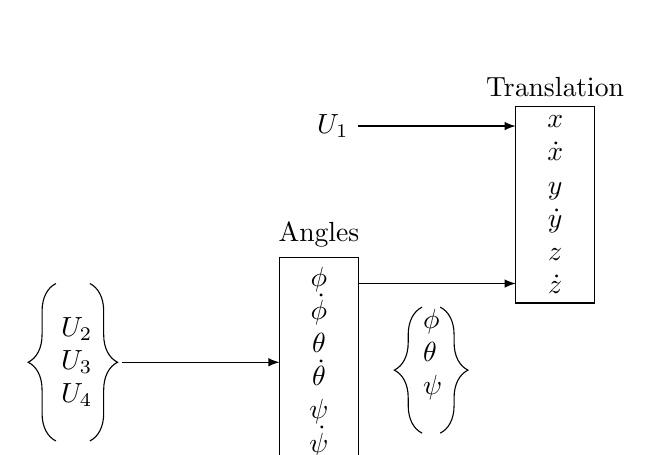
\begin{tikzpicture}
		
		%Drawing first rectangle
		\node (firstRectangle) at (0,0) [draw, rectangle, text centered, text width=1em, minimum 
		width=1cm, minimum height=2cm, label={Angles}]{$\phi$ \\ $\dot{\phi}$ \\ 
		$\theta$ \\ $\dot{\theta}$ \\ $\psi$ \\ $\dot{\psi}$};
		
		%Drawing second rectangle
		\node (secondRectangle) at (3,2) [draw, rectangle, text centered, text width=1em, minimum 
		width=1cm, minimum height=2cm, label={Translation}]{$x$ \\ $\dot{x}$ \\ $y$ \\ 
		$\dot{y}$ \\ $z$ \\ $\dot{z}$};
		
		%First arrow
		\draw[-latex] (0.5,1) coordinate -- (2.5,1) coordinate;
		\draw (1.5,0.8) coordinate node[below, text width=1em]{$\phi$ \\ $\theta$ \\ $\psi$};
		\draw [decorate,decoration={brace,amplitude=10pt,mirror,raise=4pt},yshift=0pt]
		(1.45,0.7) -- (1.45,-0.9) node [black,midway,xshift=0.8cm] {};
		\draw [decorate,decoration={brace,amplitude=10pt,raise=4pt},yshift=0pt]
		(1.40,0.7) -- (1.40,-0.9) node [black,midway,xshift=0.8cm] {};
		
		%Second arrow
		\draw[latex-] (-0.5,0) coordinate -- (-2.5,0) coordinate;
		\draw (-2.8,0) coordinate node[left, text width=1em]{$U_2$ \\ $U_3$ \\ $U_4$};
		\draw [decorate,decoration={brace,amplitude=10pt,mirror,raise=4pt},yshift=0pt]
		(-3.2,1) -- (-3.2,-1) node [black,midway,xshift=0.8cm] {};
		\draw [decorate,decoration={brace,amplitude=10pt,raise=4pt},yshift=0pt]
		(-3.05,1) -- (-3.05,-1) node [black,midway,xshift=0.8cm] {};
		
		%Third arrow
		\draw[-latex] (0.5,3) coordinate -- (2.5,3) coordinate;
		\draw (0.5,3) coordinate node[left]{$U_1$};
		
		\end{tikzpicture}
	}
	\end{center}

\end{figure}

\newpage

\section{Example \theblockDiagram}
\stepcounter{blockDiagram}

\begin{figure}[h]
	\begin{center}
			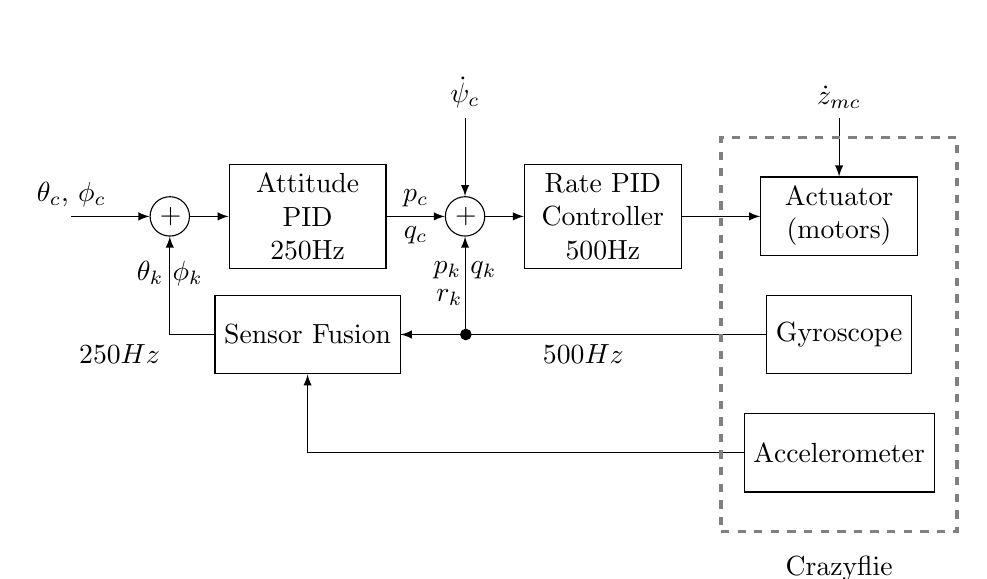
\begin{tikzpicture}
			
			%Blocks of the scheme
			\node (attitudePID) at (3.5,0) [draw, rectangle, minimum width=1cm, minimum height=1cm, 
			text centered, text width=5em]{Attitude PID\\250Hz};
			\node (ratePID) at (7.25,0) [draw, rectangle, minimum width=1cm, minimum height=1cm, 
			text centered, text width=5em]{Rate PID\\Controller\\500Hz};
			\node (actuators) at (10.25,0) [draw, rectangle, minimum width=1cm, minimum height=1cm, 
			text centered, text width=5em]{Actuator\\(motors)};
			\node (gyroscope) at (10.25,-1.5) [draw, rectangle, minimum width=1cm, minimum 
			height=1cm, text centered]{Gyroscope};
			\node (accelerometer) at (10.25,-3) [draw, rectangle, minimum width=1cm, minimum 
			height=1cm, text centered]{Accelerometer};
			\node (sensorFusion) at (3.5,-1.5) [draw, rectangle, minimum width=1cm, minimum 
			height=1cm, text centered]{Sensor Fusion};
			
			%Adders
			\node (adder1) at (1.75,0) [draw, circle, text centered, minimum size=0.5cm]{};
			\node (adder2) at (5.5,0) [draw, circle, text centered, minimum size=0.5cm]{};
			
			%Bubblies
			\node (coordinates1) at (5.51,-1.5) [circle, draw, scale=0.4, fill=black]{};
			
			%Linx
			\draw[-latex] (0.5,0) coordinate node[above]{$\theta_c$, $\phi_c$} -- (adder1);
			\draw[-latex] (adder1)   -- (attitudePID);
			\draw[-latex] (attitudePID) -- node[above]{$p_c$} node[below]{$q_c$} (adder2);
			\draw[-latex] (adder2) -- (ratePID);
			\draw[-latex] (ratePID) -- (actuators);
			\draw[-latex] (gyroscope) -- node[below]{$500Hz$} (sensorFusion);
			\draw[-latex] (accelerometer) -| (sensorFusion);
			\draw[-latex] (sensorFusion) -| (adder2);
			\draw[-latex] (sensorFusion) -| node[below left]{$250Hz$} (adder1);
			\draw[-latex] (5.5,1.25) coordinate node[above]{$\dot{\psi}_c$} -- (adder2);
			\draw[-latex] (10.25,1.25) coordinate node[above]{$\dot{z}_{mc}$} -- (actuators);
			
			%Senros fusion's outputs
			\draw (1.75,-0.45) coordinate node[below]{$\theta_k$ $\phi_k$};
			\draw (5.5,-0.45) coordinate node[below]{$p_k$ $q_k$};
			\draw (5.3,-0.8) coordinate node[below]{$r_k$};
			
			%Signs
			\draw (1.5,0) coordinate node[right]{$+$};
			\draw (5.25,0) coordinate node[right]{$+$};
			
			%Comments
			\node (Crazyflie) at (10.25,-1.5) [dashed, gray, rectangle, minimum width=3cm, 
			minimum height=5cm, draw, line width=1.25pt]{};
			\draw (10.25,-4.75) coordinate node[above]{Crazyflie};
			
			\end{tikzpicture}
	\end{center}
\end{figure}

\section{Example \theblockDiagram}
\stepcounter{blockDiagram}

\begin{figure}[h]
	\begin{center}
			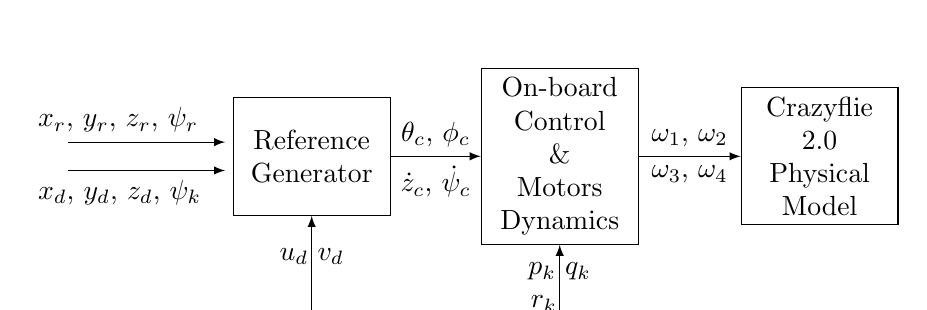
\begin{tikzpicture}
			
			%Blocks
			\node (ReferenceGenerator) at (-2.1,0) [draw, rectangle, minimum height=1.5cm, minimum 
			width=1cm, text centered, text width=5em]{Reference\\Generator};
			
			\node (OnboardCrazyflie) at (1.05,0) [draw, rectangle, minimum height=1.5cm, minimum 
			width=1cm, text centered, text width=5em]{On-board\\Control \\\& \\Motors Dynamics};
			
			\node (Crazyflie) at (4.35,0) [draw, rectangle, minimum height=1.5cm, minimum 
			width=1cm, text centered, text width=5em]{Crazyflie 2.0\\ Physical Model};
			
			%Links
			\draw[-latex] (ReferenceGenerator)  -- node[above]{$\theta_c$, $\phi_c$} 
			node[below]{$\dot{z}_c$, $\dot{\psi}_c$} (OnboardCrazyflie) ;
			\draw[-latex] (OnboardCrazyflie) -- node[above]{$\omega_1$, $\omega_2$} 
			node[below]{$\omega_3$, $\omega_4$}(Crazyflie);
			\draw[-latex] (-5.2,0.18)  -- (-3.2,0.18);
			\draw[-latex] (-5.2,-0.18) -- (-3.2,-0.18);
			\draw[-latex] (-2.1,-2.1) coordinate -- (ReferenceGenerator);
			\draw[-latex] (1.05,-2.1) coordinate -- (OnboardCrazyflie);
			\draw (0.85,-1.65) coordinate node[below]{$r_k$};
			
			%Variables
			\draw (-5.7,0.18) node[above right]{$x_r$, $y_r$, $z_r$, $\psi_r$};
			\draw (-5.7,-0.18) node[below right]{$x_d$, $y_d$, $z_d$, $\psi_k$};
			\draw (1.05,-1.7) node[above]{$p_k$ $q_k$};
			\draw (-2.1,-1.5) node[above]{$u_d$ $v_d$};
			
			\end{tikzpicture}
	\end{center}
\end{figure}


\section{Example \theblockDiagram}
\stepcounter{blockDiagram}

\begin{figure}[h]
	\begin{center}
		\scalebox{0.825}{
		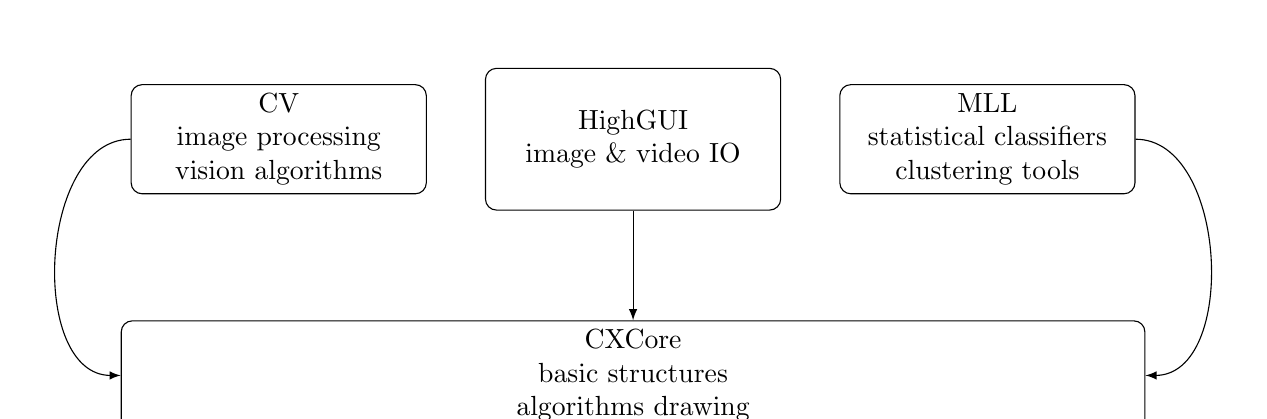
\begin{tikzpicture}
		
		%Nodes
		\node (highGUI) at (0,0) [rectangle, draw, minimum width=2cm, minimum height=1.8cm, 
		align=center, text width=10em, rounded corners]{HighGUI \\ image \& video IO};
		
		\node (CV) at (-4.5,0) [rectangle, draw, minimum width=2cm, minimum height=1cm, 
		align=center, text width=10em, rounded corners]{CV \\ image processing \\ vision 
		algorithms};
		
		\node (MLL) at (4.5,0) [rectangle, draw, minimum width=2cm, minimum height=1cm, 
		align=center, text width=10em, rounded corners]{MLL \\ statistical classifiers \\ 
		clustering tools};
		
		\node (CXCORE) at (0,-3) [rectangle, draw, minimum width=13cm, minimum height=1cm, 
		align=center, text width=10em, rounded corners]{CXCore \\ basic structures \\ algorithms 
		drawing};
		
		%Links
		\draw[-latex] (CV) to [out=180, in=180] (CXCORE);
		\draw[-latex] (highGUI.south) -- (CXCORE.90);
		\draw[-latex] (MLL) to [out=0, in=0] (CXCORE);
		
		\end{tikzpicture}
	}
	\end{center}

\end{figure}

\newpage


\section{Example \theblockDiagram}
\stepcounter{blockDiagram}

\begin{figure}[h]
	\begin{center}
		\scalebox{1}{
			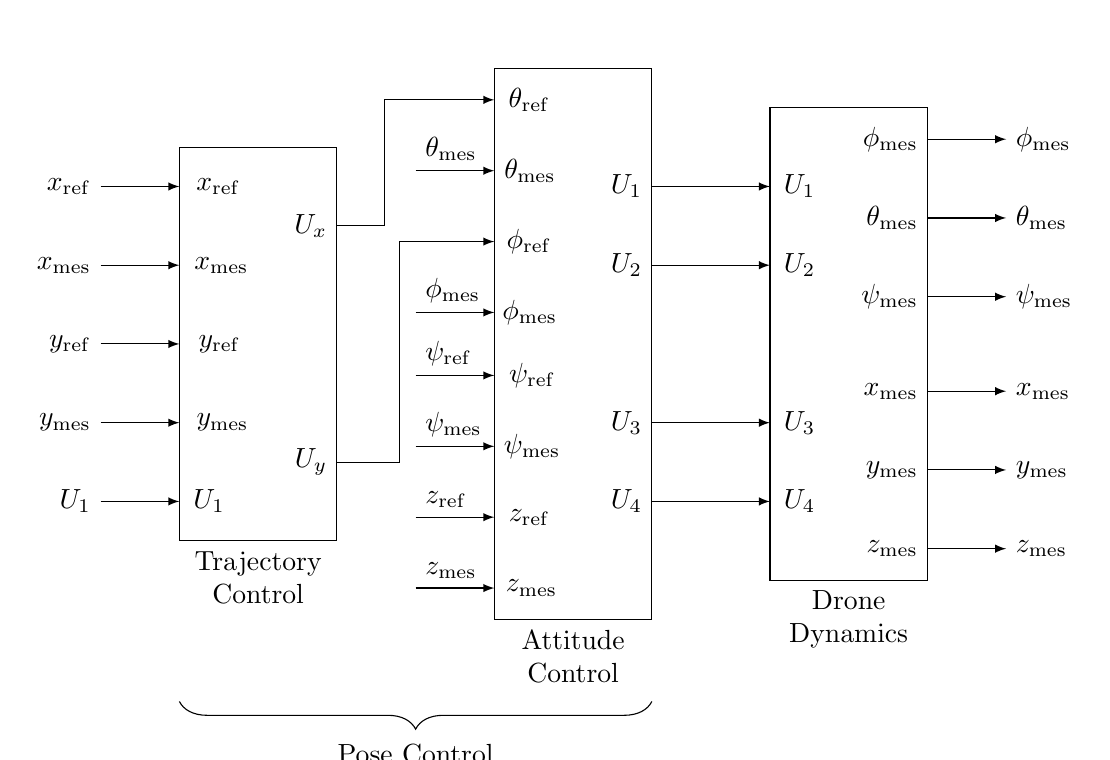
\begin{tikzpicture}
			
			%Trajectory controller
			\node (trajectoryController) at (-4,0) [draw, rectangle, minimum width=2cm, minimum 
			height=5cm, text centered, label={[align=center]below:Trajectory\\ Control}]{};
			
			%Variables
			\draw (-4.1,2.0) coordinate node[left]{$x_\mathrm{ref}$};
			\draw (-4.0,1.0) coordinate node[left]{$x_{\mathrm{mes}}$};
			\draw (-4.1,0.0) coordinate node[left]{$y_\mathrm{ref}$};
			\draw (-4.0,-1.0) coordinate node[left]{$y_{\mathrm{mes}}$};
			\draw (-4.3,-2.0) coordinate node[left]{$U_1$};
			
			\draw (-3.0,1.5) coordinate node[left]{$U_x$};
			\draw (-3.0,-1.5) coordinate node[left]{$U_y$};
			
			%Links
			\draw[-latex] (-6,2.0) coordinate node[left]{$x_\mathrm{ref}$} -- (-5,2.0) coordinate;
			\draw[-latex] (-6,1.0) coordinate node[left]{$x_{\mathrm{mes}}$} -- (-5,1.0) coordinate;
			\draw[-latex] (-6,0.0) coordinate node[left]{$y_\mathrm{ref}$} -- (-5,0.0) coordinate;
			\draw[-latex] (-6,-1.0) coordinate node[left]{$y_{\mathrm{mes}}$} -- (-5,-1.0) 
			coordinate;
			\draw[-latex] (-6,-2.0) coordinate node[left]{$U_1$} -- (-5,-2.0) coordinate; 
			
			
			%Attitude controller
			\node (attitudeController) at (0,0) [draw, rectangle, minimum width=2cm, minimum 
			height=7cm, text centered, label={[align=center]below:Attitude\\ Control}]{};
			
			%Curly brackets
			\draw [decorate,decoration={brace,mirror, amplitude=10pt,raise=4pt},yshift=0pt]
			(-5,-4.4) -- (1,-4.4) node [black,midway,xshift=0.0cm,yshift=-0.8cm] {Pose Control};
			
			%Variables
			\draw (-0.17,3.1) node[left]{$\theta_\mathrm{ref}$};
			\draw (-0.1,2.2) node[left]{$\theta_{\mathrm{mes}}$};
			\draw (-0.15,1.3) node[left]{$\phi_\mathrm{ref}$};
			\draw (-0.08,0.4) node[left]{$\phi_{\mathrm{mes}}$};
			\draw (-0.1,-0.4) node[left]{$\psi_\mathrm{ref}$};
			\draw (-0.04,-1.3) node[left]{$\psi_{\mathrm{mes}}$};
			\draw (-0.17,-2.2) node[left]{$z_\mathrm{ref}$};
			\draw (-0.08,-3.1) node[left]{$z_{\mathrm{mes}}$};
			
			\draw (1.0,2) node[left]{$U_1$};
			\draw (1.0,1) node[left]{$U_2$};
			\draw (1.0,-1) node[left]{$U_3$};
			\draw (1.0,-2) node[left]{$U_4$};
			
			%Links
			\draw[-latex] (-3.0,1.5) coordinate -- (-2.4,1.5) coordinate -- (-2.4,3.1) coordinate  
			-- (-1.0,3.1) coordinate;
			\draw[-latex] (-3,-1.5) -- (-2.2,-1.5) coordinate -- (-2.2,1.3) coordinate -- 
			(-1.0,1.3) coordinate;
			
			\draw[-latex] (-2.0,2.2) coordinate node[above right]{$\theta_{\mathrm{mes}}$} -- 
			(-1.0,2.2) coordinate;
			\draw[-latex] (-2.0,0.4) coordinate node[above right]{$\phi_{\mathrm{mes}}$} -- 
			(-1.0,0.4) coordinate;				
			\draw[-latex] (-2.0,-0.4) coordinate node[above right]{$\psi_\mathrm{ref}$} -- 
			(-1.0,-0.4) coordinate;
			\draw[-latex] (-2.0,-1.3) coordinate node[above right]{$\psi_{\mathrm{mes}}$} -- 
			(-1.0,-1.3) coordinate;	
			\draw[-latex] (-2.0,-2.2) coordinate node[above right]{$z_\mathrm{ref}$} -- (-1.0,-2.2) 
			coordinate;
			\draw[-latex] (-2.0,-3.1) coordinate node[above right]{$z_{\mathrm{mes}}$} -- 
			(-1.0,-3.1) 
			coordinate;	
			
			%Drone model block
			\node (droneMOdel) at (3.5,0) [draw, rectangle, minimum width=2cm, minimum 
			height=6cm, text centered, label={[align=center]below:Drone\\ Dynamics}]{};
			
			%variables
			\draw (3.2,2) coordinate node[left]{$U_1$};
			\draw (3.2,1) coordinate node[left]{$U_2$};
			\draw (3.2,-1) coordinate node[left]{$U_3$};
			\draw (3.2,-2) coordinate node[left]{$U_4$};
			
			\draw (4.5,2.6) coordinate node[left]{$\phi_{\mathrm{mes}}$};
			\draw (4.5,1.6) coordinate node[left]{$\theta_{\mathrm{mes}}$};
			\draw (4.5,0.6) coordinate node[left]{$\psi_{\mathrm{mes}}$};
			\draw (4.5,-0.6) coordinate node[left]{$x_{\mathrm{mes}}$};
			\draw (4.5,-1.6) coordinate node[left]{$y_{\mathrm{mes}}$};
			\draw (4.5,-2.6) coordinate node[left]{$z_{\mathrm{mes}}$};
			
			%Links
			\draw[-latex] (1.0,2) coordinate -- (2.5,2) coordinate;
			\draw[-latex] (1.0,1) coordinate -- (2.5,1) coordinate;
			\draw[-latex] (1.0,-1) coordinate -- (2.5,-1) coordinate;
			\draw[-latex] (1.0,-2) coordinate -- (2.5,-2) coordinate;
			
			\draw[-latex] (4.5,2.6) coordinate -- (5.5,2.6) coordinate 
			node[right]{$\phi_{\mathrm{mes}}$};
			\draw[-latex] (4.5,1.6) coordinate -- (5.5,1.6) coordinate 
			node[right]{$\theta_{\mathrm{mes}}$};
			\draw[-latex] (4.5,0.6) coordinate -- (5.5,0.6) coordinate 
			node[right]{$\psi_{\mathrm{mes}}$};
			\draw[-latex] (4.5,-0.6) coordinate -- (5.5,-0.6) coordinate 
			node[right]{$x_{\mathrm{mes}}$};
			\draw[-latex] (4.5,-1.6) coordinate -- (5.5,-1.6) coordinate 
			node[right]{$y_{\mathrm{mes}}$};
			\draw[-latex] (4.5,-2.6) coordinate -- (5.5,-2.6) coordinate 
			node[right]{$z_{\mathrm{mes}}$};
			
			
			\end{tikzpicture}
		}
	\end{center}
	
\end{figure}



\section{Example \theblockDiagram}
\stepcounter{blockDiagram}

\begin{figure}[h]
	\begin{center}	
		\begin{tikzpicture}
		
		%A different way to draw a block diagram
		\bXInput[$\theta_d$]{Reference}               			
		\bXComp*[2]{Comparator}{Reference}              		
		\bXLink{Reference}{Comparator}                  			
		
		\bXBloc[3]{Integrator}{$I$}{Comparator}  					
		\bXLink{Comparator}{Integrator} 							
		\bXComp*[4]{Comparator1}{Integrator}						
		\bXLink{Integrator}{Comparator1}							
		\bXBloc[2]{Proportional}{$P$}{Comparator1}				
		\bXLink{Comparator1}{Proportional}						
		\bXSuma*[4]{Comparator2}{Proportional}				 
		\bXLink{Proportional}{Comparator2}						
		\bXBloc[2]{Integrator1}{$\dfrac{1}{s}$}{Comparator2}		
		\bXLink{Comparator2}{Integrator1}							
		\bXBloc[3]{Integrator2}{$\dfrac{1}{s}$}{Integrator1}		
		\bXLink[$\dot{\theta}$]{Integrator1}{Integrator2}			
		\bXOutput{Uscita}{Integrator2}								
		\bXLink[$\theta$]{Integrator2}{Uscita}						
		\bXReturn[5]{Integrator2-Uscita}{Comparator}{}			
		\bXReturn{Integrator1-Integrator2}{Comparator1}{}	    
		\bXBranchy[-4]{Comparator-Integrator}{Proportional2}	
		\bXChain[1.5]{Proportional2}{p/$P$}						
		\bXLinkyx{Comparator-Integrator}{p}						
		\bXLinkxy{p}{Comparator2}								
		
		\end{tikzpicture}
	\end{center}
\end{figure}



\newpage

\section{Example \theblockDiagram}
\stepcounter{blockDiagram}

\begin{figure}[h]
	\begin{center}
		\scalebox{0.75}{
			\begin{tikzpicture}
						
			\node (pd1) at (0,0) [draw, rectangle, text centered, minimum width=1.5cm, minimum 
			height=1cm]{$\text{PD}_\theta$};
			
			\node (adder1) at (-2,0) [draw, circle, text centered, minimum size=0.5cm]{};
			
			\draw[-latex] (-2,-1.5) coordinate node[below]{$\theta_{\mathrm{mes}}$} -- 
			(adder1.south);
			\draw[-latex] (adder1.east) node[above right]{$e_\theta$} -- (pd1.west);
			\draw[-latex] (-3,0) coordinate node[left]{$\theta_\mathrm{ref}$}-- (adder1.west);
			
			\draw (-2.05,0.15) coordinate node[above left]{$+$};
			\draw (-2.05,-0.25) coordinate node[below right]{$-$};
			
			\node (pd2) at (0,-3.0) [draw, rectangle, text centered, minimum width=1.5cm, minimum 
			height=1cm]{$\text{PD}_\phi$};
			
			\node (adder2) at (-2,-3.0) [draw, circle, text centered, minimum size=0.5cm]{};
			
			\draw[-latex] (-2,-4.5) coordinate node[below]{$\phi_{\mathrm{mes}}$} -- (adder2.south);
			\draw[-latex] (adder2.east) node[above right]{$e_\phi$} -- (pd2.west);
			\draw[-latex] (-3,-3) coordinate node[left]{$\phi_\mathrm{ref}$} -- (adder2.west);
			
			\draw (-2.05,-2.85) coordinate node[above left]{$+$};
			\draw (-2.05,-3.25) coordinate node[below right]{$-$};
			
			\node (pd3) at (0,-6.0) [draw, rectangle, text centered, minimum width=1.5cm, minimum 
			height=1cm]{$\text{PD}_\psi$};
			
			\node (adder3) at (-2,-6.0) [draw, circle, text centered, minimum size=0.5cm]{};
			
			\draw[-latex] (-2,-7.5) coordinate node[below]{$\psi_{\mathrm{mes}}$} -- (adder3.south);
			\draw[-latex] (adder3.east) node[above right]{$e_\psi$} -- (pd3.west);
			\draw[-latex] (-3,-6) coordinate node[left]{$\psi_\mathrm{ref}$} -- (adder3.west);
			
			\draw (-2.05,-5.85) coordinate node[above left]{$+$};
			\draw (-2.05,-6.25) coordinate node[below right]{$-$};
			
			\node (pd4) at (0,-9.0) [draw, rectangle, text centered, minimum width=1.5cm, minimum 
			height=1cm]{$\text{PD}_z$};
			
			\node (adder4) at (-2,-9.0) [draw, circle, text centered, minimum size=0.5cm]{};
			
			\draw[-latex] (-2,-10.5) coordinate node[below]{$z_{\mathrm{mes}}$} -- (adder4.south);
			\draw[-latex] (adder4.east) node[above right]{$e_z$} -- (pd4.west);
			\draw[-latex] (-3,-9) coordinate node[left]{$z_\mathrm{ref}$} -- (adder4.west);
			
			\draw (-2.05,-8.85) coordinate node[above left]{$+$};
			\draw (-2.05,-9.25) coordinate node[below right]{$-$};
			
			
			\node (droneModel) at (3,-4.5) [draw, rectangle, minimum height=11cm, minimum 
			width=2cm, text centered, text 		
			width=1em]{D\\R\\O\\N\\E\\$\hspace{0.1cm}$\\M\\O\\D\\E\\L\\};
			
			\draw[-latex] (pd1.east) node [above right]{$U_3$} -- (2.0,0.0) coordinate;
			\draw[-latex] (pd2.east) node [above right]{$U_2$} -- (2.0,-3.0) coordinate;
			\draw[-latex] (pd3.east) node [above right]{$U_4$} -- (2.0,-6.0) coordinate;
			\draw[-latex] (pd4.east) node [above right]{$U_1$} -- (2.0,-9.0) coordinate;
			
			\draw[-latex] (4.0,0) coordinate -- (5,0) coordinate 
			node[right]{$\theta_{\mathrm{mes}}$};
			\draw[-latex] (4.0,-3) coordinate -- (5,-3) coordinate 
			node[right]{$\phi_{\mathrm{mes}}$};
			\draw[-latex] (4.0,-6) coordinate -- (5,-6) coordinate 
			node[right]{$\psi_{\mathrm{mes}}$};
			\draw[-latex] (4.0,-9) coordinate -- (5,-9) coordinate node[right]{$z_{\mathrm{mes}}$};
			
			
			\end{tikzpicture}
		}
	\end{center}
	
\end{figure}

\section{Example \theblockDiagram}
\stepcounter{blockDiagram}

\begin{figure}[h]
	\begin{center}
		\scalebox{0.8}{
			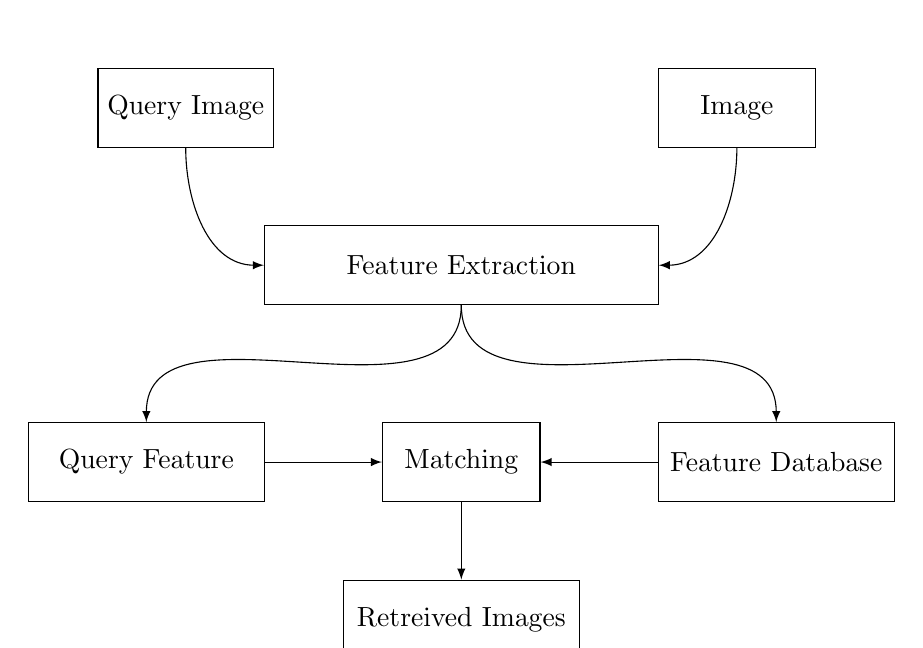
\begin{tikzpicture}[node distance=2cm]
			
			%Nodes	
			\node (queryImage) at (-3.5, 0) [rectangle, draw, text centered, minimum width=2cm, 
			minimum height=1cm] {Query Image};
			
			\node (image) at ( 3.5, 0) [rectangle, text centered, draw, minimum width=2cm, minimum 
			height=1cm] {Image};
			
			\node (featureExtraction) at ( 0,-2) [rectangle, draw, text centered, minimum 
			width=5cm, minimum height=1cm] {Feature Extraction};
			
			\node (queryFeature) at (-4,-4.5) [rectangle, draw, text centered, minimum width=3cm, 
			minimum height=1cm] {Query Feature};
			
			\node (matching) at ( 0,-4.5) [rectangle, draw, text centered, minimum width=2cm, 
			minimum height=1cm] {Matching};
			
			\node (featureDatabase) at ( 4,-4.5) [rectangle, draw, text centered, minimum 
			width=3cm, minimum height=1cm] {Feature Database};
			
			\node (retreivedImages) at ( 0,-6.5) [rectangle, draw, text centered, minimum 
			width=3cm, minimum height=1cm] {Retreived Images};
			
			%Links
			\draw [-latex] (queryFeature.east) -- (matching.west);
			\draw [-latex] (featureDatabase.west) -- (matching.east);
			\draw [-latex] (matching.south) -- (retreivedImages.north);
			\draw [-latex] (queryImage) to [out=270,in=180] (featureExtraction);
			\draw [-latex] (image) to [out=270,in=0] (featureExtraction);
			\draw [-latex] (featureExtraction) to [out=270,in=90] (queryFeature);
			\draw [-latex] (featureExtraction) to [out=270,in=90] (featureDatabase);
			
			\end{tikzpicture}
		}
	\end{center}
\end{figure}

\newpage

\section{Example \theblockDiagram}
\stepcounter{blockDiagram}

\begin{figure}[h]
	\begin{center}
		\scalebox{0.95}{
		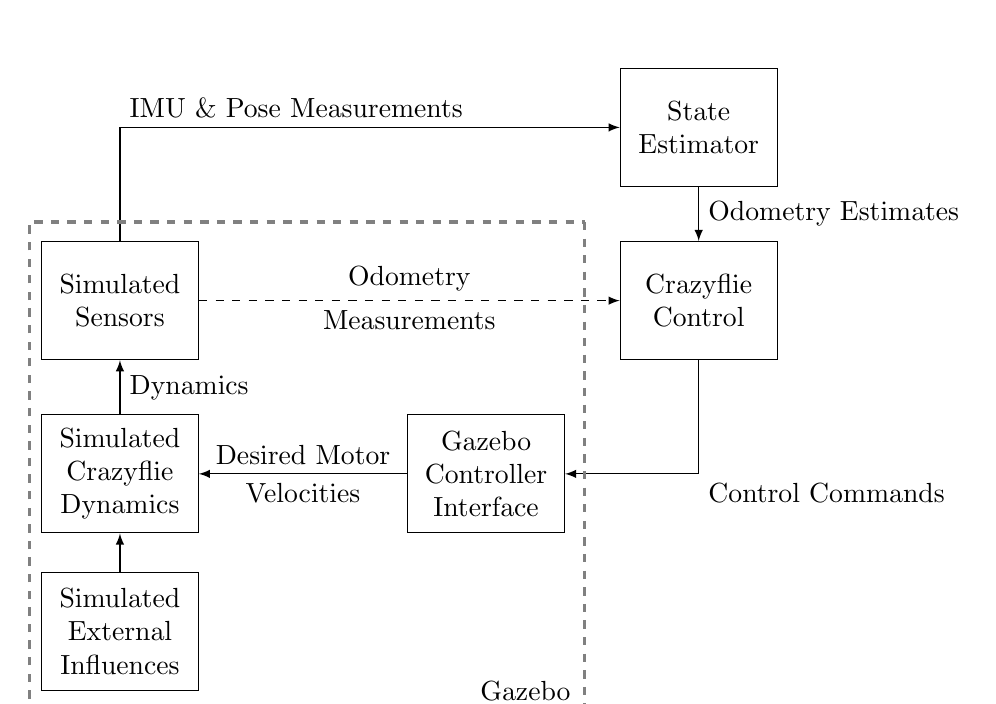
\begin{tikzpicture}
		
		%Blocks
		\node (CrazyflieControl) at (0.2,0) [draw, rectangle, minimum width=1.5cm, minimum 
		height=1.5cm, text centered, text width=5em]{Crazyflie Control};
		\node (GazeboControllerInterface) at (-2.5,-2.2) [draw, rectangle, minimum width=1.5cm, 
		minimum height=1.5cm, text centered, text width=5em]{Gazebo Controller\\Interface};
		\node (SimulatedExternalInfluence) at (-7.15,-4.2) [draw, rectangle, minimum 
		width=1.5cm, minimum height=1.5cm, text centered, text width=5em]{Simulated 
		External\\Influences};
		\node (SimulatedCrazyflieDynamics) at (-7.15,-2.2) [draw, rectangle, minimum 
		width=1.5cm, minimum height=1.5cm, text centered, text width=5em]{Simulated 
		Crazyflie\\Dynamics};
		\node (SimulatedSensor) at (-7.15,0) [draw, rectangle, minimum width=1.5cm, minimum 
		height=1.5cm, text centered, text width=5em]{Simulated Sensors};
		\node (StateEstimator) at (0.2,2.2) [draw, rectangle, minimum width=1.5cm, minimum 
		height=1.5cm, text centered, text width=5em]{State Estimator};
		
		%Links
		\draw[-latex] (CrazyflieControl) |- node[below right]{Control Commands} 
		(GazeboControllerInterface);
		\draw[-latex] (GazeboControllerInterface) -- node[above]{Desired Motor} 
		node[below]{Velocities} (SimulatedCrazyflieDynamics);
		\draw[-latex] (SimulatedExternalInfluence) -- (SimulatedCrazyflieDynamics);
		\draw[-latex] (SimulatedSensor) |- node[above right]{IMU \& Pose Measurements} 
		(StateEstimator);
		\draw[-latex] (StateEstimator) -- node[right]{Odometry Estimates} (CrazyflieControl);
		\draw[-latex] (SimulatedCrazyflieDynamics) -- node[right] {Dynamics} (SimulatedSensor);
		\draw[-latex, dashed] (SimulatedSensor) -- node[above]{Odometry} 
		node[below]{Measurements} (CrazyflieControl) ;
		
		%Gazebo's group
		\draw[dashed, gray, draw, line width=1.25pt] (-1.25,1) coordinate -- (-1.25,-5.25) 
		coordinate -- (-8.3,-5.25) coordinate -- (-8.3,1) coordinate -- (-1.25,1) coordinate; 
		\draw (-2,-5.2) coordinate node[above]{Gazebo};
		
		\end{tikzpicture}
	}
	\end{center}
\end{figure}



\section{Example \theblockDiagram}
\stepcounter{blockDiagram}

\begin{figure}[h]
	\begin{center}
		\scalebox{0.9}{
			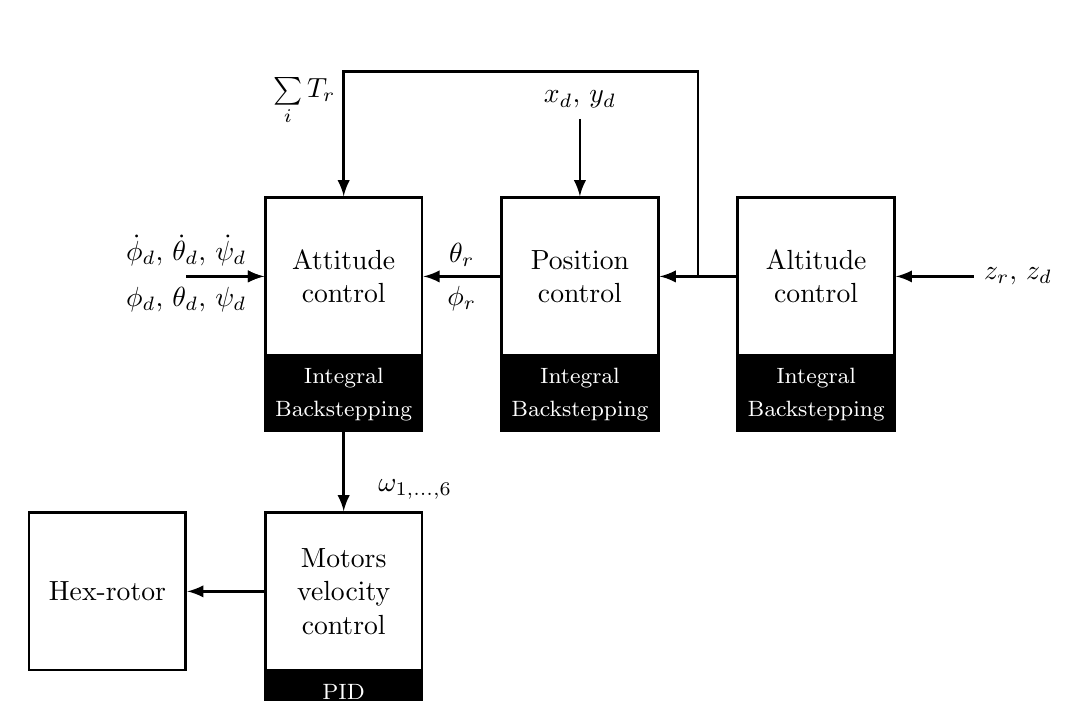
\begin{tikzpicture}
			
			%Attitude controller
			\node (attitudeController) at (-3,0) [draw, rectangle, text centered, line width=1.0pt, 
			minimum height=2cm, minimum width=1cm, text width=5em]{Attitude\\ control};
			
			%baseline Integral Backstepping
			\node (baselineIntegralBackstepping) at (-3,-1.50) [draw, line width=1.0pt, fill=black, 
			rectangle, minimum height=0.5cm, minimum width=1cm, text centered, text 
			width=5em]{\footnotesize{\color{white}{Integral\\ Backstepping}}}; 
			
			%PositionController
			\node (positionController) at (0,0) [draw, rectangle, line width=1.0pt, text centered, 
			minimum height=2cm, minimum width=1cm, text width=5em]{Position\\ control};
			
			%Baseline Integral Backstepping
			\node at (0,-1.50) [draw, line width=1.0pt, fill=black, rectangle, minimum 
			height=0.5cm, minimum width=1cm, text centered, text 
			width=5em]{\footnotesize{\color{white}{Integral\\ Backstepping}}}; 
			
			%Altitude controller
			\node (altitudeController) at (3,0) [draw, rectangle, line width=1.0pt, text centered, 
			minimum height=2cm, minimum width=1cm, text width=5em]{Altitude\\ control};
			
			%Baseline Integral Backstepping
			\node at (3,-1.50) [draw, line width=1.0pt, fill=black, rectangle, minimum 
			height=0.5cm, minimum width=1cm, text centered, text 
			width=5em]{\footnotesize{\color{white}{Integral\\ Backstepping}}}; 
			
			%Motors controller
			\node (motorsController) at (-3,-4) [draw, rectangle, line width=1.0pt, text 
			centered, minimum height=2cm, minimum width=1cm, text width=5em]{Motors velocity 
			control};
			
			%Baseline PID
			\node at (-3,-5.28) [draw, line width=1.0pt, fill=black, rectangle, minimum 
			height=0.5cm, minimum width=1cm, text centered, text 
			width=5em]{\footnotesize{\color{white}{PID}}}; 
			
			%Hexarotor
			\node (hexarotor) at (-6,-4) [draw, rectangle, line width=1.0pt, text centered, 
			minimum height=2cm, minimum width=1cm, text width=5em]{Hex-rotor};
			
			%Links
			\draw[-latex, line width=1.0pt] (motorsController.west) -- (hexarotor.east);
			\draw[-latex, line width=1.0pt] (altitudeController.west) -- (positionController.east);
			\draw[-latex, line width=1.0pt] (positionController.west) -- (attitudeController.east);
			\draw[-latex, line width=1.0pt] (baselineIntegralBackstepping.south) -- 
			(motorsController.north);
			
			\draw[-latex, line width=1.0pt] (1.5,0) coordinate -- (1.5,2.6) coordinate -- (-3,2.6) 
			coordinate -- (attitudeController.north);
			
			%Reference signals
			\draw[-latex, line width=1.0pt] (5,0) coordinate node[right]{$z_r,\,z_d$}-- 
			(altitudeController.east);
			\node[above] at (-3.5,1.8) [text centered]{$\sum\limits_i T_r$};
			\draw[-latex, line width=1.0pt] (0,2) coordinate node[above]{$x_d,\,y_d$} -- 
			(positionController.north);
			\node[above] at (-1.5,0) [text centered]{$\theta_r$};
			\node[below] at (-1.5,0) [text centered]{$\phi_r$};
			\draw[-latex, line width=1.0pt] (-5.0,0) coordinate 
			node[below]{$\phi_d,\,\theta_d,\,\psi_d$} -- (attitudeController.west);
			\draw[-latex, line width=1.0pt] (-5.0,0) coordinate 
			node[above]{$\dot{\phi}_d,\,\dot{\theta}_d,\,\dot{\psi}_d$} -- 
			(attitudeController.west);
			\node at (-1.5,-2.7) [left, text centered]{$\omega_{1,\dots,6}$}; 
			
			\end{tikzpicture}
		}
	\end{center}
	
	
\end{figure}

\newpage




\section{Example \theblockDiagram}
\stepcounter{blockDiagram}

\begin{figure}[h]
	\begin{center}
		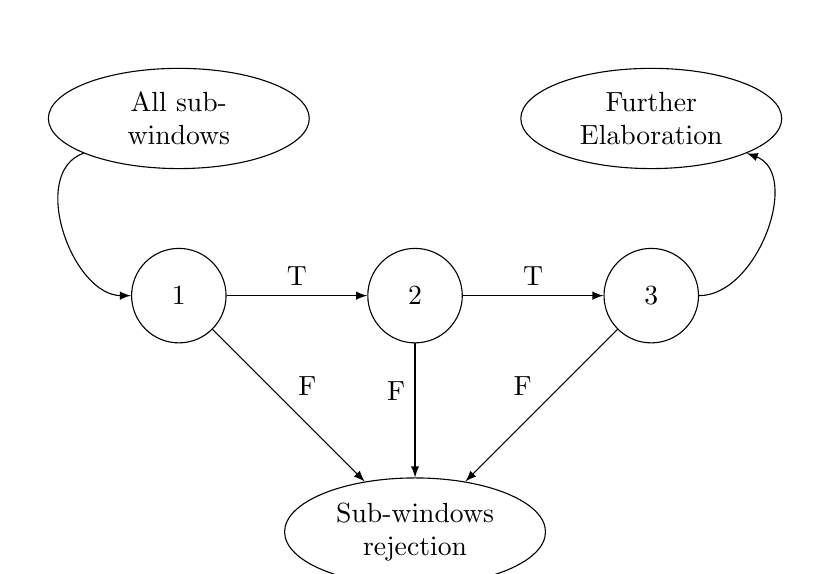
\begin{tikzpicture}[node distance=2cm]
		
		%Creo i nodi del diagramma di flusso		
		\node (allSubWindow) at (-3,1) [ellipse, draw, text centered, text width=6em] {All 
		sub-windows};
		
		\node (furtherProcessing) at (3,1) [ellipse, draw, text centered, text width=6em] {Further 
		Elaboration};
		
		\node (1) at (-3,-1.25) [circle, draw, text centered, minimum size=1.2cm] {1};
		
		\node (2) at (0,-1.25) [circle, draw, text centered, minimum size=1.2cm] {2};
		
		\node (3) at (3,-1.25) [circle, draw, text centered, minimum size=1.2cm] {3};
		
		\node (rejectSubWindows) at (0,-4.25) [ellipse, draw, text centered, text width=6em] 
		{Sub-windows rejection};
		
		\draw[-latex] (1) -- node[above]{T} (2);
		\draw[-latex] (2) -- node[above]{T} (3);
		\draw[-latex] (2) -- node[above left]{F} (rejectSubWindows);
		\draw[-latex] (1) -- node[above right]{F} (rejectSubWindows);
		\draw[-latex] (3) -- node[above left]{F} (rejectSubWindows);
		\draw[-latex] (allSubWindow) to [out=200,in=180] (1);
		\draw[-latex] (3) to [out=0, in=340] (furtherProcessing);
		
		\end{tikzpicture}
	\end{center}
	
\end{figure}

\section{Example \theblockDiagram}
\stepcounter{blockDiagram}

\begin{figure}[h]
	\begin{center}
		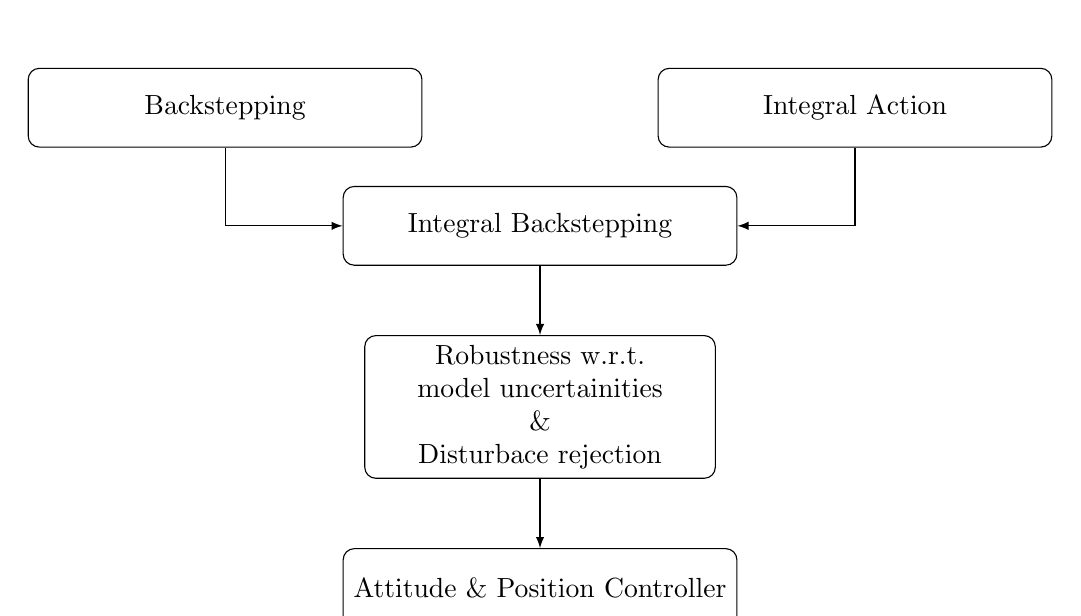
\begin{tikzpicture}
		
		%Nodes
		\node (BackStepping) at (-4,1.5) [draw, rectangle, minimum height=1cm, minimum width=5cm, 
		text centered, rounded corners]{Backstepping};
		\node (integralAction) at (4,1.5) [draw, rectangle, minimum height=1cm, minimum width=5cm, 
		text centered, rounded corners]{Integral Action};
		
		%Rappresento il nodo centrale
		\node (integralBackStepping) at (0,0) [draw, rectangle, minimum height=1cm, minimum 
		width=5cm, text centered, rounded corners]{Integral Backstepping};
		
		%Rappresento il blocco caratteristiche
		\node (features) at (0,-2.3) [draw, rectangle, minimum height=1cm, minimum 
		width=1cm, text centered, rounded corners, text width=12em]{Robustness w.r.t. model 
		uncertainities\\ \& \\Disturbace rejection};
		
		%Control system results
		\node (results) at (0,-4.6) [draw, rectangle, minimum height=1cm, minimum width=5cm, text 
		centered, rounded corners]{Attitude \& Position Controller};
		
		%Links
		\draw[-latex] (BackStepping.270) -- (-4,0) coordinate -- (integralBackStepping.180);
		\draw[-latex] (integralAction.270) -- (4,0) coordinate -- (integralBackStepping.0);
		\draw[-latex] (integralBackStepping.south) -- (features.north);
		\draw[-latex] (features.south) -- (results.north);
		
		
		\end{tikzpicture}
	\end{center}
	
\end{figure}

\newpage


\section{Example \theblockDiagram}
\stepcounter{blockDiagram}

\begin{figure}[h]
	\begin{center}
		\scalebox{0.8}{
		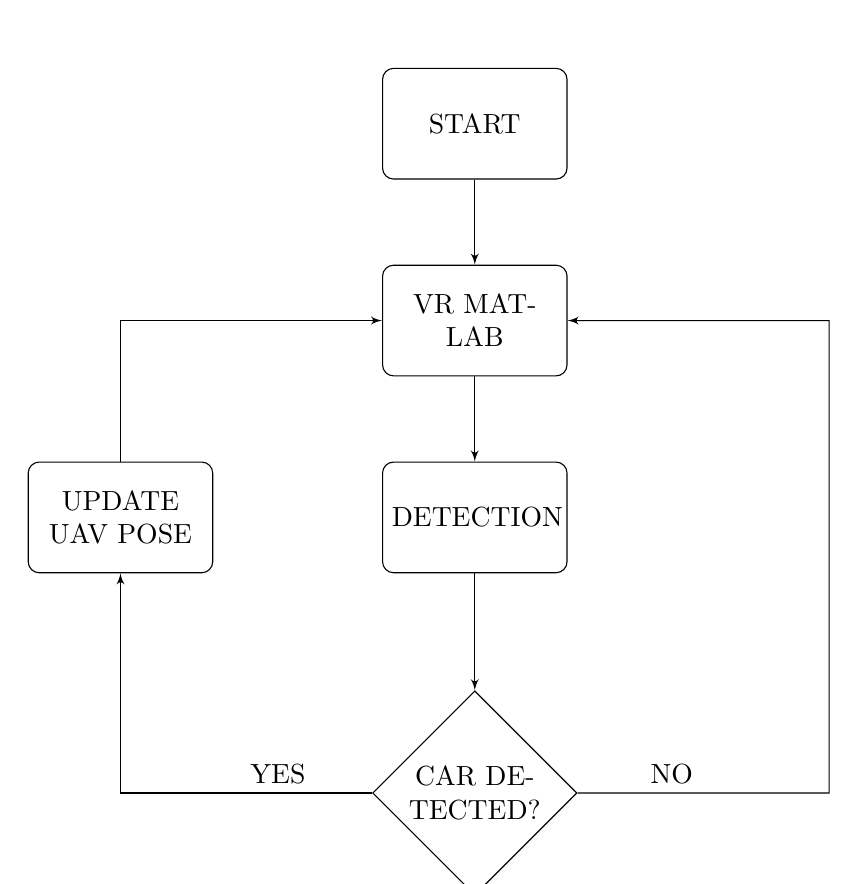
\begin{tikzpicture}
		
		%System nodes
		\node [rectangle, draw, text width=6em, text centered, rounded corners, minimum height=4em] 
		(start) at (0,0) {START};
		
		\node [rectangle, draw, text width=6em, text centered, rounded corners, minimum height=4em, 
		below of=init] (vrMatlab) at (0,-1.5) {VR MATLAB};
		
		\node [rectangle, draw, text width=6em, text centered, rounded corners, minimum height=4em, 
		below of=identify] (detection) at (0,-4.0) {DETECTION};
		
		\node [rectangle, draw, text width=6em, text centered, rounded corners, minimum height=4em, 
		left of=evaluate, node distance=3cm] (update) at (-1.5,-5) {UPDATE UAV POSE};
		
		\node [diamond, draw, text width=5.5em, text badly centered, node distance=3cm, inner 
		sep=0pt, below of=evaluate] (decide) at (0,-5.5) {CAR DETECTED?};
		
		
		%Links
		\path [draw, -latex'] (start) -- (vrMatlab);
		\path [draw, -latex'] (vrMatlab) -- (detection);
		\path [draw, -latex'] (detection) -- (decide);
		\path [draw, -latex'] (decide) -| (update);
		\path [draw, -latex'] (update) |- (vrMatlab);
		\path [draw, -latex'] (decide.east) -- (4.5,-8.5) coordinate -- (4.5,-2.5) coordinate -- 
		(vrMatlab.east);
		
		%Decisions
		\node at (2.5,-8.5)  [above] {NO};
		\node at (-2.5,-8.5) [above] {YES};
		
		\end{tikzpicture}
	}
	\end{center}
	
\end{figure}

\newpage

\section{Example \theblockDiagram}
\stepcounter{blockDiagram}

\begin{figure}[h]
	\begin{center}
		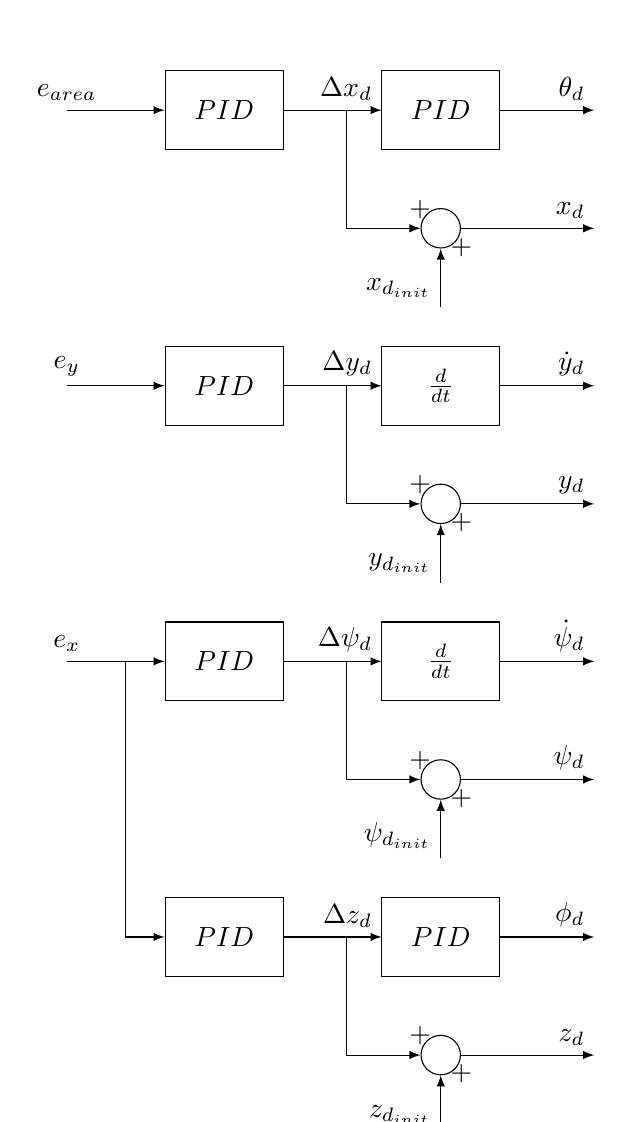
\begin{tikzpicture}
		
		%Nodes
		\node (firstPID) at (-2,0.5) [draw, rectangle, minimum width=1.5cm, minimum height=1cm, 
		text centered]{$PID$};
		
		\node (secondPID) at (0.75,0.5) [draw, text centered, minimum width=1.5cm, minimum 
		height=1cm]{$PID$};
		
		\node (adder) at (0.75,-1) [draw, circle, text centered, minimum size=0.5cm]{};
		
		%Links
		\draw[-latex] (-4,0.5) coordinate node[above]{$e_{area}$} -- (firstPID.west);
		
		\draw[-latex] (firstPID.east) -- (0,0.5) coordinate node[above left]{$\Delta x_d$};
		
		\draw[-latex] (secondPID.east) -- (2.7,0.5) coordinate node[above left]{$\theta_d$};
		
		\draw[-latex] (-0.45,0.5) coordinate -- (-0.45,-1) coordinate -- (adder.west);
		
		\draw[-latex] (adder.east) -- (2.7,-1) coordinate node[above left]{$x_d$};
		
		\draw[-latex] (0.75,-2.0) coordinate node[above left]{$x_{d_{init}}$} -- (adder.south);
		
		%Signs
		\draw (0.75,-1) coordinate node[above left]{$+$};
		\draw (0.75,-1) coordinate node[below right]{$+$};
		
		%Names into the second part of the scheme
		\node (thirdPID) at (-2,-3.0) [draw, rectangle, minimum width=1.5cm, minimum height=1cm, 
		text centered]{$PID$};
		
		\node (fourthPID) at (0.75,-3.0) [draw, text centered, minimum width=1.5cm, minimum 
		height=1cm]{$\frac{d}{dt}$};
		
		\node (adder1) at (0.75,-4.5) [draw, circle, text centered, minimum size=0.5cm]{};
		
		%Links among blocks
		\draw[-latex] (-4,-3.0) coordinate node[above]{$e_y$} -- (thirdPID.west);
		
		\draw[-latex] (thirdPID.east) -- (0,-3.0) coordinate node[above left]{$\Delta y_d$};
		
		\draw[-latex] (fourthPID.east) -- (2.7,-3.0) coordinate node[above left]{$\dot{y}_d$};
		
		\draw[-latex] (-0.45,-3.0) coordinate -- (-0.45,-4.5) coordinate -- (adder1.west);
		
		\draw[-latex] (adder1.east) -- (2.7,-4.5) coordinate node[above left]{$y_d$};
		
		\draw[-latex] (0.75,-5.5) coordinate node[above left]{$y_{d_{init}}$} -- (adder1.south);
		
		%Signs
		\draw (0.75,-4.5) coordinate node[above left]{$+$};
		\draw (0.75,-4.5) coordinate node[below right]{$+$};
		
		%Third part of the scheme
		\node (fifthPID) at (-2,-6.5) [draw, rectangle, minimum width=1.5cm, minimum height=1cm, 
		text centered]{$PID$};
		
		\node (sixthPID) at (0.75,-6.5) [draw, text centered, minimum width=1.5cm, minimum 
		height=1cm]{$\frac{d}{dt}$};
		
		\node (adder2) at (0.75,-8.0) [draw, circle, text centered, minimum size=0.5cm]{};
		
		%Links among blocks
		\draw[-latex] (-4,-6.5) coordinate node[above]{$e_x$} -- (fifthPID.west);
		
		\draw[-latex] (fifthPID.east) -- (0,-6.5) coordinate node[above left]{$\Delta \psi_d$};
		
		\draw[-latex] (sixthPID.east) -- (2.7,-6.5) coordinate node[above left]{$\dot{\psi}_d$};
		
		\draw[-latex] (-0.45,-6.5) coordinate -- (-0.45,-8.0) coordinate -- (adder2.west);
		
		\draw[-latex] (adder2.east) -- (2.7,-8.0) coordinate node[above left]{$\psi_d$};
		
		\draw[-latex] (0.75,-9.0) coordinate node[above left]{$\psi_{d_{init}}$} -- 
		(adder2.south);
		
		%Signs
		\draw (0.75,-8.0) coordinate node[above left]{$+$};
		\draw (0.75,-8.0) coordinate node[below right]{$+$};
		
		
		%Signs
		\node (seventhPID) at (-2,-10) [draw, rectangle, minimum width=1.5cm, minimum height=1cm, 
		text centered]{$PID$};
		
		\node (eighthPID) at (0.75,-10) [draw, text centered, minimum width=1.5cm, minimum 
		height=1cm]{$PID$};
		
		\node (adder3) at (0.75,-11.5) [draw, circle, text centered, minimum size=0.5cm]{};
		
		%Links
		\draw[-latex] (-3.25,-6.5) coordinate -- (-3.25,-10) coordinate -- (seventhPID.west);
		
		\draw[-latex] (seventhPID.east) -- (0,-10) coordinate node[above left]{$\Delta z_d$};
		
		\draw[-latex] (eighthPID.east) -- (2.7,-10) coordinate node[above left]{$\phi_d$};
		
		\draw[-latex] (-0.45,-10) coordinate -- (-0.45,-11.5) coordinate -- (adder3.west);
		
		\draw[-latex] (adder3.east) -- (2.7,-11.5) coordinate node[above left]{$z_d$};
		
		\draw[-latex] (0.75,-12.5) coordinate node[above left]{$z_{d_{init}}$} -- (adder3.south);
		
		%Signs
		\draw (0.75,-11.5) coordinate node[above left]{$+$};
		\draw (0.75,-11.5) coordinate node[below right]{$+$};
		\end{tikzpicture}
	\end{center}
	
\end{figure}
\chapter{Various}
\label{chapter:various}

\newcounter{various}
\setcounter{various}{0}
\stepcounter{various}

\section{Example \thevarious}
\stepcounter{various}

\begin{figure}[h]
	\begin{center}
		\scalebox{0.5}{
			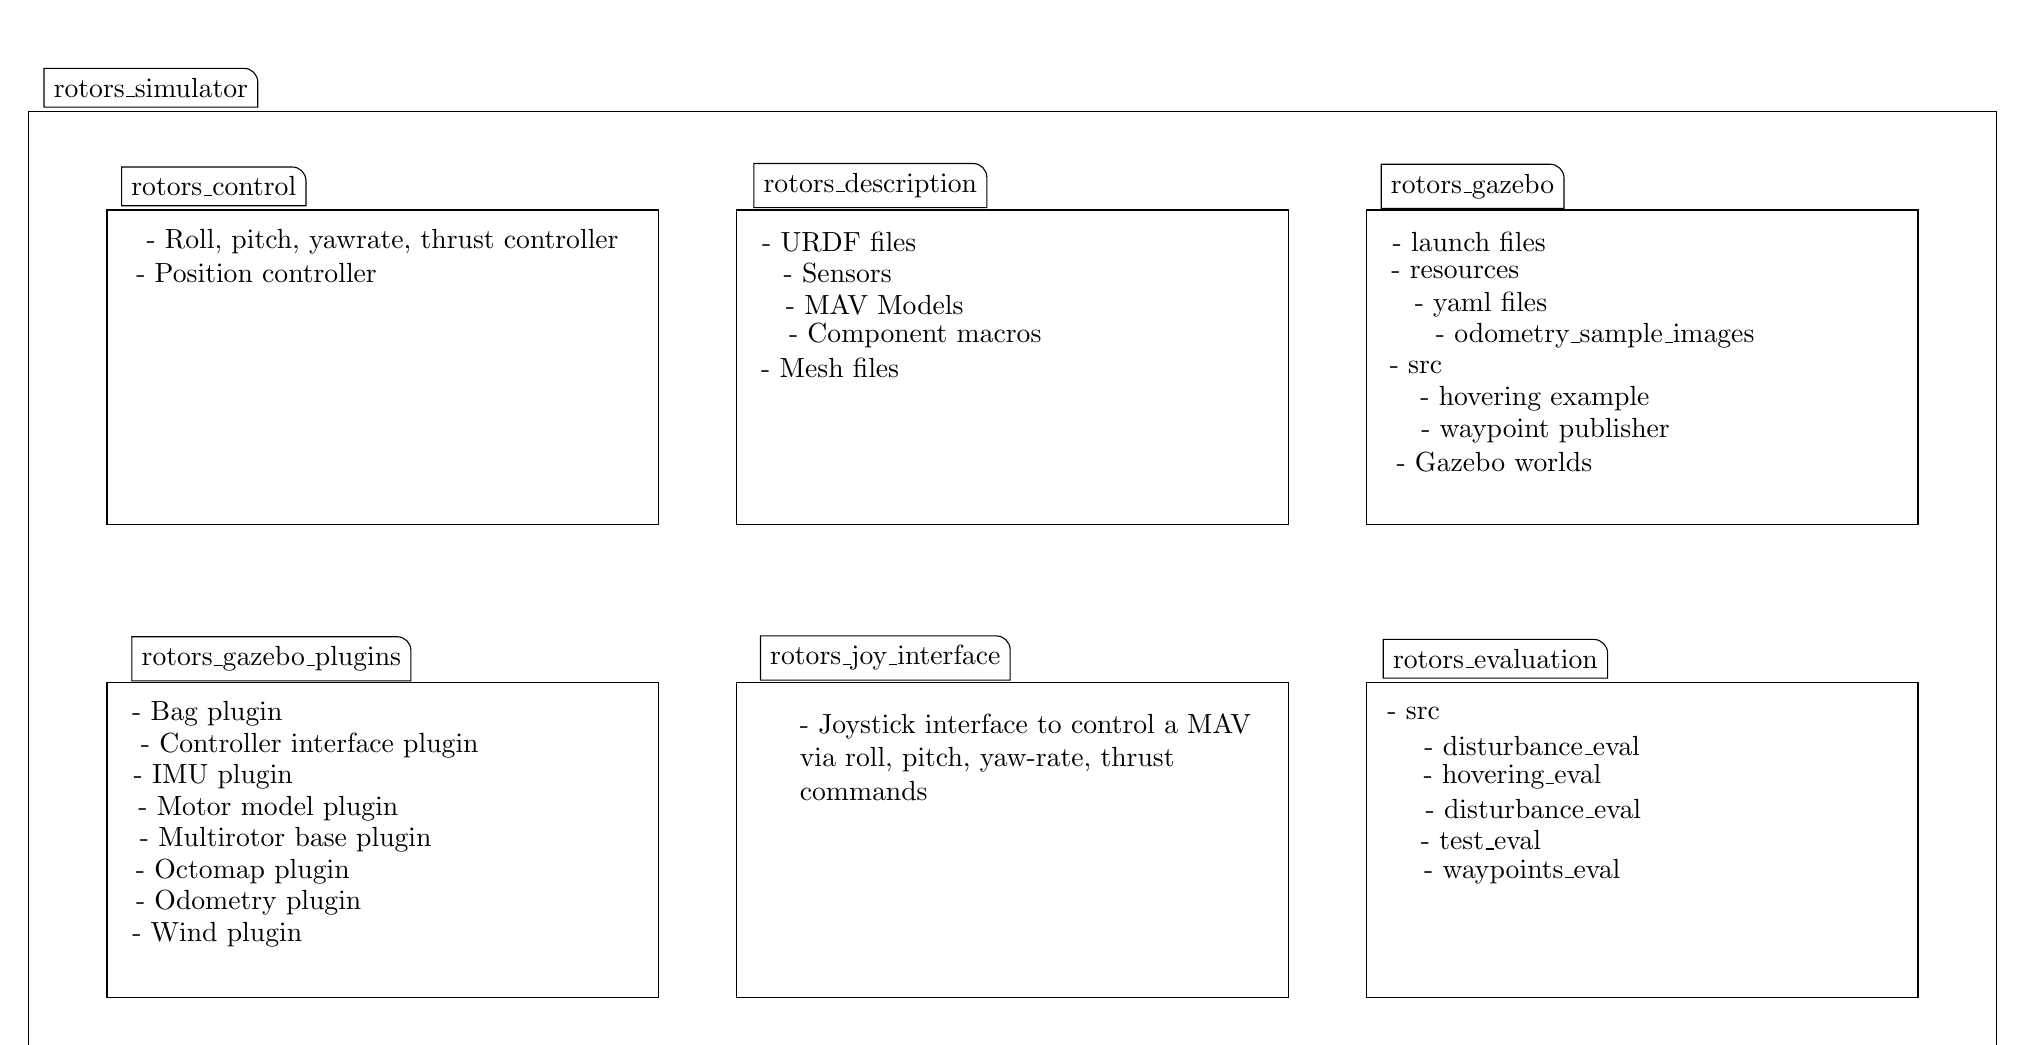
\begin{tikzpicture}
			
			%Package comments
			\node (Rotors Control) at (0,0) [draw, rectangle, minimum height=4cm, minimum 
			width=7cm, text centered]{};
			\draw node at (-2.1435,2.3)[
			append after command={[rounded corners=0pt](b.west)|-(b.north)},
			append after command={[rounded corners=5pt](b.north)-|(b.east)},
			append after command={[rounded corners=0pt](b.east)|-(b.south)},
			append after command={[rounded corners=0pt](b.south)-|(b.west)}] 
			(b) {rotors\_control};
			
			%Writing in the box
			\node at (0,1.6) [text centered]{- Roll, pitch, yawrate, thrust controller};
			\node at (-1.6,1.2) [text centered]{- Position controller};
			
			%Second block
			\node (Rotors Description) at (8,0) [draw, rectangle, minimum height=4cm, minimum 
			width=7cm, text centered]{};
			\draw node at (6.195,2.31)[
			append after command={[rounded corners=0pt](b.west)|-(b.north)},
			append after command={[rounded corners=5pt](b.north)-|(b.east)},
			append after command={[rounded corners=0pt](b.east)|-(b.south)},
			append after command={[rounded corners=0pt](b.south)-|(b.west)}] 
			(b) {rotors\_description};
			
			%Writing in the box
			\node at (5.8,1.6) [text centered]{- URDF files};
			\node at (5.78,1.2) [text centered]{- Sensors};
			\node at (6.25,0.8) [text centered]{- MAV Models};
			\node at (6.765,0.4) [text centered]{- Component macros};
			\node at (5.685,0) [text centered]{- Mesh files};
			
			%Third block
			\node (Rotors Gazebo) at (16,0) [draw, rectangle, minimum height=4cm, minimum 
			width=7cm, text centered]{};
			\draw node at (13.8435,2.3)[
			append after command={[rounded corners=0pt](b.west)|-(b.north)},
			append after command={[rounded corners=5pt](b.north)-|(b.east)},
			append after command={[rounded corners=0pt](b.east)|-(b.south)},
			append after command={[rounded corners=0pt](b.south)-|(b.west)}] 
			(b) {rotors\_gazebo};
			
			%Writing in the box
			\node at (13.8,1.6) [text centered]{- launch files};
			\node at (13.625,1.2) [text centered]{- resources};
			\node at (13.95,0.8) [text centered]{- yaml files};
			\node at (15.4,0.4) [text centered]{- odometry\_sample\_images};
			\node at (13.125,0.0) [text centered]{- src};
			\node at (14.635,-0.4) [text centered]{- hovering example};
			\node at (14.77,-0.8) [text centered]{- waypoint publisher};
			\node at (14.12,-1.2) [text centered]{- Gazebo worlds};
			
			%Fourth block
			\node (Rotors Control) at (0,-6) [draw, rectangle, minimum height=4cm, minimum 
			width=7cm, text centered]{};
			\draw node at (-1.4115,-3.7)[
			append after command={[rounded corners=0pt](b.west)|-(b.north)},
			append after command={[rounded corners=5pt](b.north)-|(b.east)},
			append after command={[rounded corners=0pt](b.east)|-(b.south)},
			append after command={[rounded corners=0pt](b.south)-|(b.west)}] 
			(b) {rotors\_gazebo\_plugins};
			
			%Writing in the box
			\node at (-2.225,-4.4) [text centered]{- Bag plugin};
			\node at (-0.925,-4.8) [text centered]{- Controller interface plugin};
			\node at (-2.15,-5.2) [text centered]{- IMU plugin};
			\node at (-1.45,-5.6) [text centered]{- Motor model plugin};
			\node at (-1.23,-6.0) [text centered]{- Multirotor base plugin};
			\node at (-1.775,-6.4) [text centered]{- Octomap plugin};
			\node at (-1.7,-6.8) [text centered]{- Odometry plugin};
			\node at (-2.1,-7.2) [text centered]{- Wind plugin};
			
			
			%Fifth block
			\node (Rotors Joy Interface) at (8,-6) [draw, rectangle, minimum height=4cm, minimum 
			width=7cm, text centered]{};
			\draw node at (6.385,-3.69)[
			append after command={[rounded corners=0pt](b.west)|-(b.north)},
			append after command={[rounded corners=5pt](b.north)-|(b.east)},
			append after command={[rounded corners=0pt](b.east)|-(b.south)},
			append after command={[rounded corners=0pt](b.south)-|(b.west)}] 
			(b) {rotors\_joy\_interface};
			
			%Writing in the box
			\node at (11.45,-4.95) [text width=35em]{- Joystick interface to control a MAV\\via 
			roll, pitch, yaw-rate, thrust\\commands};
			
			%Sixth block
			\node (Rotors Evaluation) at (16,-6) [draw, rectangle, minimum height=4cm, minimum 
			width=7cm, text centered]{};
			\draw node at (14.1335,-3.70)[
			append after command={[rounded corners=0pt](b.west)|-(b.north)},
			append after command={[rounded corners=5pt](b.north)-|(b.east)},
			append after command={[rounded corners=0pt](b.east)|-(b.south)},
			append after command={[rounded corners=0pt](b.south)-|(b.west)}] 
			(b) {rotors\_evaluation};
			
			%Writing in the box
			\node at (13.095,-4.4) [text centered]{- src};
			\node at (14.6,-4.8) [text centered]{- disturbance\_eval};
			\node at (14.35,-5.2) [text centered]{- hovering\_eval};
			\node at (14.615,-5.6) [text centered]{- disturbance\_eval};
			\node at (13.95,-6.0) [text centered]{- test\_eval};
			\node at (14.475,-6.4) [text centered]{- waypoints\_eval};
			
			%Container
			\node (container) at (8,-2.75) [draw, rectangle, minimum height=12cm, minimum 
			width=25cm]{};
			\draw node at (-2.9421,3.5525)[
			append after command={[rounded corners=0pt](b.west)|-(b.north)},
			append after command={[rounded corners=5pt](b.north)-|(b.east)},
			append after command={[rounded corners=0pt](b.east)|-(b.south)},
			append after command={[rounded corners=0pt](b.south)-|(b.west)}] 
			(b) {rotors\_simulator};
			
			\end{tikzpicture}
		}
	\end{center}

\end{figure}

\section{Example \thevarious}
\stepcounter{various}

\begin{figure}[h]
	\begin{center}
		\scalebox{0.8}{
		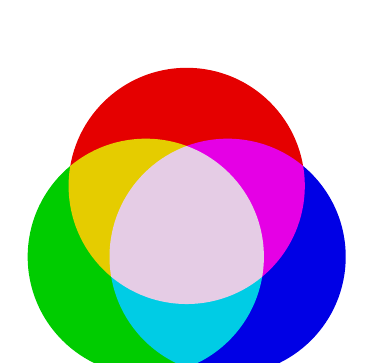
\begin{tikzpicture}[blend group=screen]
		\fill[red!90!black]   ( 90:.6) circle (1.5);
		\fill[green!80!black] (210:.6) circle (1.5);
		\fill[blue!90!black] (330:.6) circle (1.5);
		\end{tikzpicture}
	}
	\end{center}
\end{figure}

\newpage


\section{Example \thevarious}
\stepcounter{various}

\begin{figure}[h]
	\begin{center}
		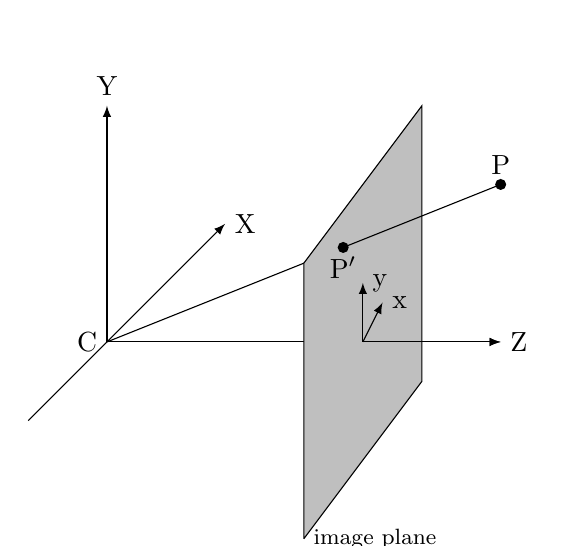
\begin{tikzpicture}
		
		\draw[-latex] (0,0) node[anchor=east]{C} -- (5,0) node[anchor=west] {Z};
		\draw[-latex] (0,0) -- (0,3) node[anchor=south] {Y};
		\draw[-latex] (-1.0,-1.0) -- (1.5,1.5) node[anchor=west] {X};
		\draw (0,0) -- (3,1.2);
		\filldraw[fill=lightgray] (2.5,-2.5) -- (2.5,1) --  (4,3) -- (4,-0.5) -- (2.5,-2.5);
		\draw[-latex] (3.25,0) -- (3.25,0.75) node[anchor=west] {y};
		\draw[-latex] (3.25,0) -- (3.5,0.5) node[anchor=west] {x};
		\draw[-latex] (3.25,0) -- (5,0);
		\draw (3,1.2) -- (5,2);
		\fill (5,2) circle[radius=2pt] node[anchor=south] {P};
		\fill (3,1.2) circle[radius=2pt] node[anchor=north] {P$'$};
		\draw (2.5,-2.5) node[anchor=west, font=\footnotesize] {image plane};
		
		\end{tikzpicture}
	\end{center}
	
\end{figure}


\section{Example \thevarious}
\stepcounter{various}

\begin{figure}[h]
	\begin{center}
		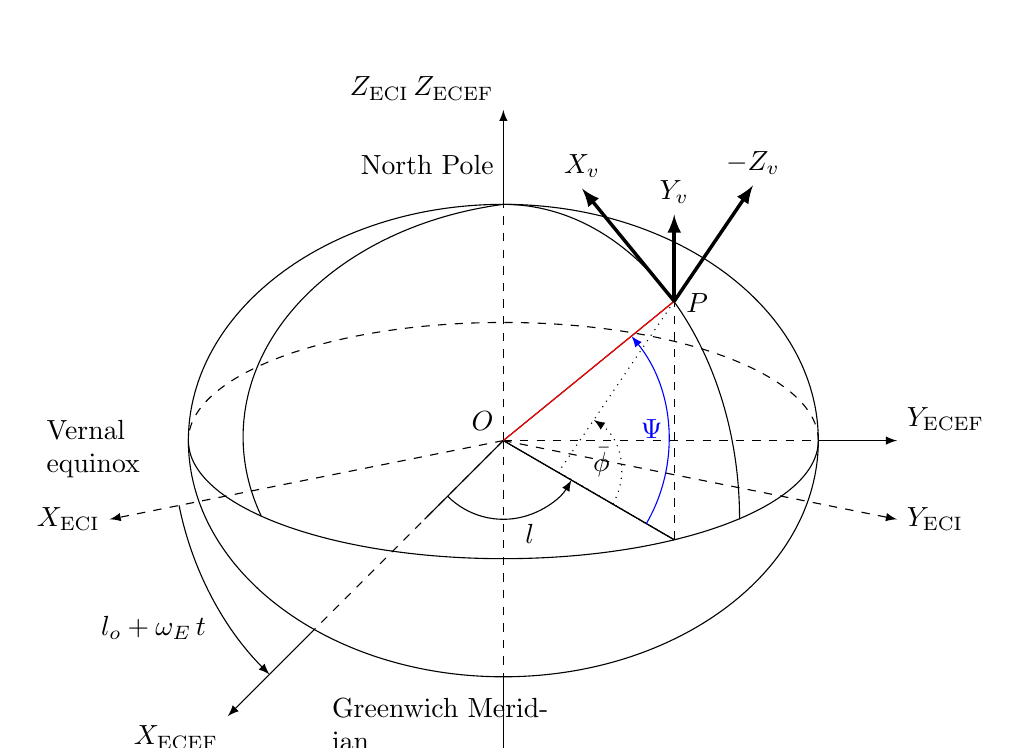
\begin{tikzpicture}
		
		%Reference system
		\draw[dashed] (0,0) coordinate -- (0,3) coordinate;
		\draw[-latex] (0,3) coordinate -- (0,4.2) coordinate node[above 
		left]{$Z_\mathrm{ECI}\,Z_\mathrm{ECEF}$};
		\draw (0,3.25) node[above left]{North Pole};
		\draw[dashed] (0,0) coordinate -- (-2.45,-2.45) coordinate;
		\draw[-latex] (-2.45,-2.45) coordinate -- (-3.5,-3.5) coordinate node [below 
		left]{$X_\mathrm{ECEF}$};
		\draw[-latex, dashed] (0,0) coordinate -- (-5,-1) coordinate node[left]{$X_\mathrm{ECI}$};
		\draw (-2.3,-3.6) node[right, text width=3cm]{Greenwich Meridian};
		\draw[dashed] (0,0) coordinate -- (4,0);
		\draw[-latex] (4,0) coordinate -- (5,0) coordinate node [above right]{$Y_\mathrm{ECEF}$};
		\draw[-latex, dashed] (0,0) coordinate -- (5.0,-1) coordinate node[right]{$Y_\mathrm{ECI}$};
		\draw (-4.8,-0.6) node[above, text width=2cm]{Vernal equinox};
		
		%First line and angle
		\draw[-] (-1,-1) coordinate (a) -- (0,0) coordinate (b) -- (2.17,-1.26) coordinate (c)
		pic[right,"$l$", draw, -latex, angle eccentricity=1.2, angle radius=1cm]{angle=a--b--c};
		
		%Second line and angle
		\draw[dotted] (2.17,-1.26) coordinate (d) -- (0.70,-0.40) coordinate (e) -- (2.17,1.77) 
		coordinate (f)
		pic["$\bar{\phi}$", draw, -latex, angle eccentricity=0.7, angle 
		radius=0.8cm]{angle=d--e--f};
		
		%Third line and angle
		\draw[-] (2.17,-1.26) coordinate (g) -- (0,0) coordinate (h) -- (2.17,1.77) coordinate (i)
		pic["$\Psi$", draw, blue, -latex, angle eccentricity=0.9, angle 
		radius=2.1cm]{angle=g--h--i};
		
		%Fourth line and angle
		\coordinate (l) at (-5,-1);
		\coordinate (m) at (0,0); 
		\coordinate (n) at (-3.5,-3.5);
		\draw pic["$l_o+\omega_E\,t$", draw, -latex, angle eccentricity=1.2, angle 
		radius=4.2cm]{angle=l--m--n};
		
		%Horizontal axis
		\draw (0,0) ellipse (4cm and 3cm);
		
		%Vertical ellipse
		\draw[dashed] (4,0) arc (0:180:4cm and 1.5cm);
		\draw (-4,0) arc (180:360:4cm and 1.5cm);
		
		%Arcs
		\draw[] (0,3) arc (100:199.5:4cm and 3cm);
		\draw (0,3) arc (90:0):3cm and 4cm);
		
		%Z-axis dashed
		\draw[dashed] (0,0) coordinate -- (0,-3) coordinate;
		\draw (0,-3) coordinate -- (0,-4) coordinate;
		
		%Reference system origin
		\draw (0,0) coordinate node[above left]{$O$};
		\draw[-, red] (0,0) coordinate -- (2.17,1.77) coordinate;
		\draw (2.2,1.5) coordinate node[above right]{$P$};
		\draw[dashed] (2.17,-1.26) coordinate -- (2.17,1.77) coordinate;
		
		%Second reference system
		\draw[-latex,line width=1.25pt] (2.17,1.77) coordinate -- (3.17,3.24) coordinate 
		node[above]{$-Z_v$};
		\draw[-latex,line width=1.25pt] (2.17,1.77) coordinate -- (1,3.2) coordinate 
		node[above]{$X_v$};
		\draw[-latex,line width=1.25pt] (2.17,1.77) coordinate -- (2.17,2.87) coordinate 
		node[above]{$Y_v$};
		
		\end{tikzpicture}
	\end{center}
	
\end{figure}

\newpage


\section{Example \thevarious}
\stepcounter{various}

\begin{figure}[h]
	\begin{center}
		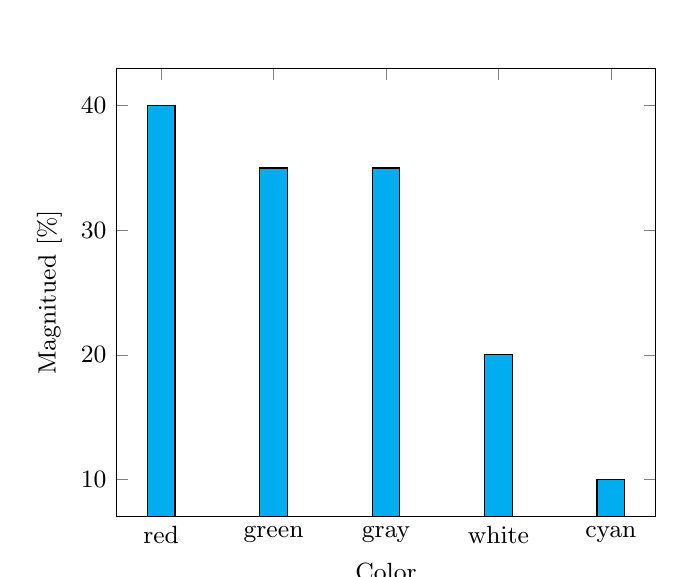
\begin{tikzpicture}[font=\small]
		
		%Histogram
		\begin{axis}[
		symbolic x coords={red, green, gray, white, cyan},
		ylabel = {Magnitued [$\%$]},
		xlabel = {Color},
		xtick=data
		]
		\addplot[ybar,draw=black, fill=cyan] coordinates {
			(red,  40)
			(green,  35)
			(gray, 35)
			(white, 20)
			(cyan,  10)
		};
		\end{axis}
		
		\end{tikzpicture}
	\end{center}
	
\end{figure}


\section{Example \thevarious}
\stepcounter{various}

\begin{figure}[h]
	\begin{center}
		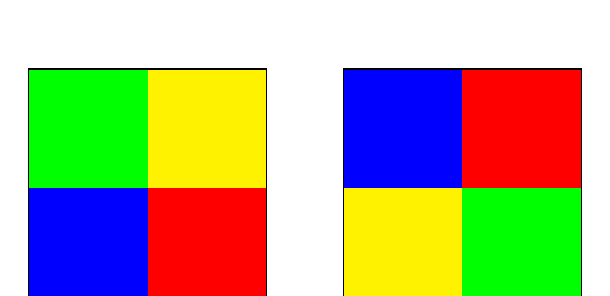
\begin{tikzpicture}
		
		%First squre
		\node (square) at (-2,0) [rectangle, draw, minimum width=3cm, minimum height=3cm, text 
		centered, line width=1.25pt]{};
		
		%Square divider
		\node (firstLine) at (-2.75, 0.75) [rectangle, fill=green, minimum width=1.5cm, minimum 
		height=1.5cm, text centered]{};
		\node (secondLine) at (-1.25, 0.75) [rectangle, fill=yellow, minimum width=1.5cm, minimum 
		height=1.5cm, text centered]{};
		\node (thirdLine) at (-2.75, -0.75) [rectangle, fill=blue, minimum width=1.5cm, minimum 
		height=1.5cm, text centered]{};
		\node (fourthLine) at (-1.25, -0.75) [rectangle, fill=red, minimum width=1.5cm, minimum 
		height=1.5cm, text centered]{};
		
		%Second squre
		\node (square2) at (2,0) [rectangle, draw, minimum width=3cm, minimum height=3cm, text 
		centered, line width=1.25pt]{};
		
		%Square divider
		\node (firstLine1) at (2.75, 0.75) [rectangle, fill=red, minimum width=1.5cm, minimum 
		height=1.5cm, text centered]{};
		\node (secondLine1) at (1.25, 0.75) [rectangle, fill=blue, minimum width=1.5cm, minimum 
		height=1.5cm, text centered]{};
		\node (thirdLine1) at (2.75, -0.75) [rectangle, fill=green, minimum width=1.5cm, minimum 
		height=1.5cm, text centered]{};
		\node (fourthLine1) at (1.25, -0.75) [rectangle, fill=yellow, minimum width=1.5cm, minimum 
		height=1.5cm, text centered]{};
		
		\end{tikzpicture}
	\end{center}
	
\end{figure}



\section{Example \thevarious}
\stepcounter{various}

\begin{figure}[h]
	\begin{center}
		\scalebox{0.8}{
		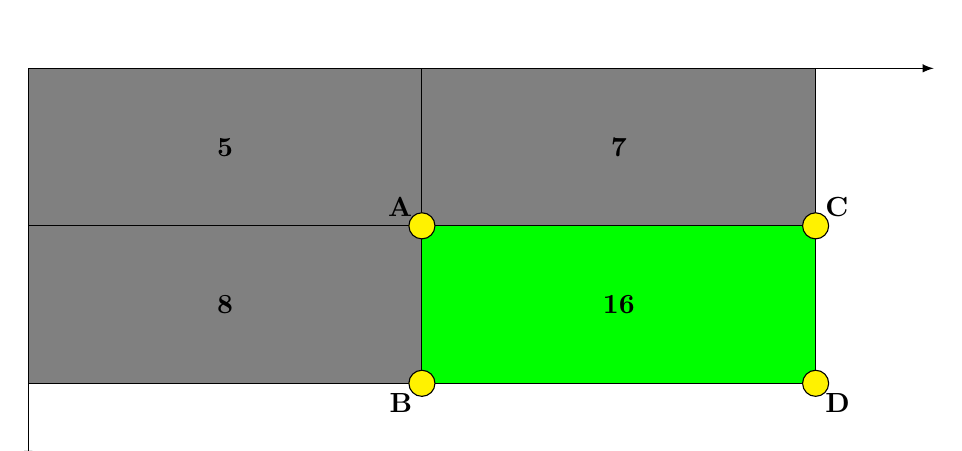
\begin{tikzpicture}
		
		%Squares
		\node (firstSquare) at (-5,5) [rectangle, draw, text centered, text width=6em, minimum 
		width=5cm, minimum height=2cm, fill=gray] {\textbf{5}};
		\node (secondSquare) at (0,5) [rectangle, draw, text centered, text width=6em, minimum 
		width=5cm, minimum height=2cm, fill=gray] {\textbf{7}};
		\node (thirdSquare) at (-5,3) [rectangle, draw, text centered, text width=6em, minimum 
		width=5cm, minimum height=2cm, fill=gray] {\textbf{8}};
		\node (fourthSquare) at (0,3) [rectangle, draw, text centered, text width=6em, minimum 
		width=5cm, minimum height=2cm, fill=green] {\textbf{16}};
		
		%Circles
		\node (firstCircle) at (-2.5,4) [circle, draw, text centered, minimum size=0.2cm, 
		fill=yellow]{};
		\node (secondCircle) at (-2.5,2) [circle, draw, text centered, minimum size=0.2cm, 
		fill=yellow]{};
		\node (thirdCircle) at (2.5,4) [circle, draw, text centered, minimum size=0.2cm, 
		fill=yellow]{};
		\node (fourthCircle) at (2.5,2) [circle, draw, text centered, minimum size=0.2cm, 
		fill=yellow]{};
		
		%Axes
		\draw[-latex] (-7.5,6) coordinate -- (4,6) coordinate;
		\draw[-latex] (-7.5,6) coordinate -- (-7.5,1) coordinate;
		
		%Letters
		\draw (-2.5, 4) coordinate node[above left]{\textbf{A}};
		\draw (2.5, 4) coordinate node[above right]{\textbf{C}};
		\draw (-2.5, 2) coordinate node[below left]{\textbf{B}};
		\draw (2.5, 2) coordinate node[below right]{\textbf{D}};
		
		\end{tikzpicture}
	}
	\end{center}
	
\end{figure}

\newpage

\section{Example \thevarious}
\stepcounter{various}

\begin{figure}[h]
	\begin{center}
		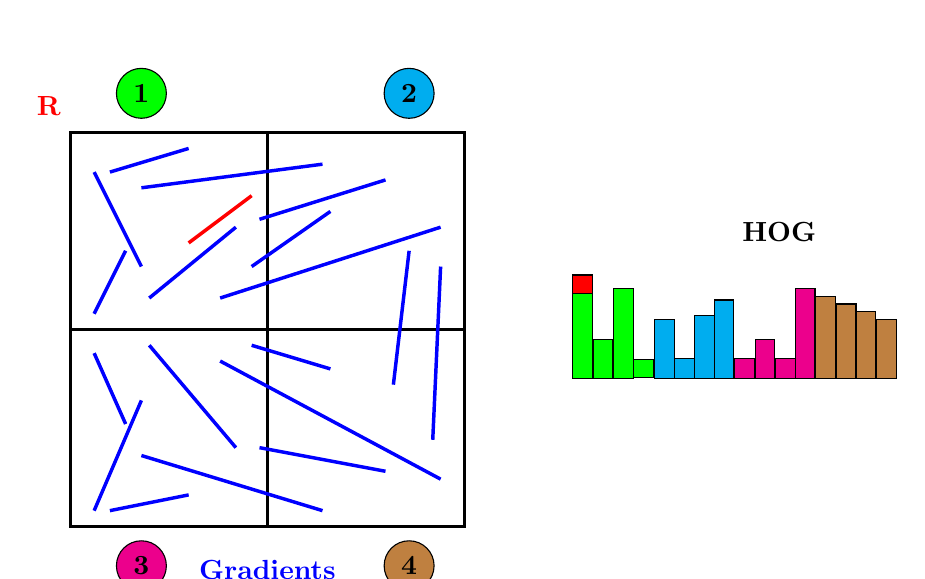
\begin{tikzpicture}
		
		%First squre
		\node (square) at (-5,0) [rectangle, draw, minimum width=5cm, minimum height=5cm, text 
		centered, line width=1.25pt]{};
		
		%Square divider
		\draw[-, line width=1.25pt] (-5,2.5) coordinate -- (-5, -2.5) coordinate;
		\draw[-, line width=1.25pt] (-7.5,0) coordinate -- (-2.5,0);
		
		%Lines
		\draw[-, blue, line width=1.25pt] (-7.2,0.2) coordinate -- (-6.8,1.0) coordinate;
		\draw[-, blue, line width=1.25pt] (-6.5, 0.4) coordinate -- (-5.4, 1.3) coordinate;
		\draw[-, blue, line width=1.25pt] (-6.6, 0.8) coordinate -- (-7.2, 2.0) coordinate;
		\draw[-, blue, line width=1.25pt] (-5.6, 0.4) coordinate -- (-2.8, 1.3) coordinate;
		\draw[-, blue, line width=1.25pt] (-5.2, 0.8) coordinate -- (-4.2, 1.5) coordinate;
		\draw[-, blue, line width=1.25pt] (-5.1, 1.4) coordinate -- (-3.5, 1.9) coordinate;
		\draw[-, blue, line width=1.25pt] (-7.0, 2.0) coordinate -- (-6.0, 2.3) coordinate;
		\draw[-, blue, line width=1.25pt] (-6.6, 1.8) coordinate -- (-4.3, 2.1) coordinate;
		
		\draw[-, blue, line width=1.25pt] (-7.2,-0.3) coordinate -- (-6.8, -1.2) coordinate;
		\draw[-, blue, line width=1.25pt] (-6.5, -0.2) coordinate -- (-5.4, -1.5) coordinate;
		\draw[-, blue, line width=1.25pt] (-6.6, -0.9) coordinate -- (-7.2, -2.3) coordinate;
		\draw[-, blue, line width=1.25pt] (-5.6, -0.4) coordinate -- (-2.8, -1.9) coordinate;
		\draw[-, blue, line width=1.25pt] (-5.2, -0.2) coordinate -- (-4.2, -0.5) coordinate;
		\draw[-, blue, line width=1.25pt] (-5.1, -1.5) coordinate -- (-3.5, -1.8) coordinate;
		\draw[-, blue, line width=1.25pt] (-7.0, -2.3) coordinate -- (-6.0, -2.1) coordinate;
		\draw[-, blue, line width=1.25pt] (-6.6, -1.6) coordinate -- (-4.3, -2.3) coordinate;
		
		\draw[-, blue, line width=1.25pt] (-2.8, 0.8) coordinate -- (-2.9, -1.4) coordinate;
		\draw[-, blue, line width=1.25pt] (-3.2, 1.0) coordinate -- (-3.4, -0.7) coordinate;
		
		\draw[-, red, line width=1.25pt] (-6.0, 1.1) coordinate -- (-5.2, 1.7) coordinate;
		
		%Histogram
		\node (rectangle1) at (-1,-0.05) [rectangle, draw, minimum width=0.25cm, fill=green, 
		minimum height=1.15cm, text centered]{};
		\node (rectangle) at (-1,0.575) [rectangle, draw, minimum width=0.25cm, fill=red, minimum 
		height=0.15cm, text centered]{};
		\node (rectangle2) at (-0.74,-0.375) [rectangle, draw, fill=green, minimum width=0.25cm, 
		minimum height=0.5cm, text centered]{};
		\node (rectangle3) at (-0.48,-0.05) [rectangle, draw, fill=green, minimum width=0.25cm, 
		minimum height=1.15cm, text centered]{};
		\node (rectangle4) at (-0.22,-0.497) [rectangle, draw, fill=green, minimum width=0.25cm, 
		minimum height=0.15cm, text centered]{};
		\node (rectangle5) at (0.04,-0.25) [rectangle, draw, fill=cyan, minimum width=0.25cm, 
		minimum height=0.75cm, text centered]{};
		\node (rectangle6) at (0.30,-0.497) [rectangle, draw, fill=cyan, minimum width=0.25cm, 
		minimum height=0.25cm, text centered]{};
		\node (rectangle7) at (0.55,-0.225) [rectangle, draw, fill=cyan, minimum width=0.25cm, 
		minimum height=0.80cm, text centered]{};
		\node (rectangle8) at (0.80,-0.125) [rectangle, draw, fill=cyan, minimum width=0.25cm, 
		minimum height=1.00cm, text centered]{};
		\node (rectangle9) at (1.06,-0.497) [rectangle, draw, minimum width=0.25cm, fill=magenta, 
		minimum height=0.25cm, text centered]{};
		\node (rectangle10) at (1.32,-0.375) [rectangle, draw, fill=magenta, minimum width=0.25cm, 
		minimum height=0.5cm, text centered]{};
		\node (rectangle11) at (1.58,-0.497) [rectangle, draw, fill=magenta, minimum width=0.25cm, 
		minimum height=0.25cm, text centered]{};
		\node (rectangle12) at (1.83,-0.05) [rectangle, draw, fill=magenta, minimum width=0.25cm, 
		minimum height=1.15cm, text centered]{};
		\node (rectangle13) at (2.09,-0.1) [rectangle, draw, fill=brown, minimum width=0.25cm, 
		minimum height=1.05cm, text centered]{};
		\node (rectangle14) at (2.35,-0.15) [rectangle, draw, fill=brown, minimum width=0.25cm, 
		minimum height=0.95cm, text centered]{};
		\node (rectangle15) at (2.60,-0.2) [rectangle, draw, fill=brown, minimum width=0.25cm, 
		minimum height=0.85cm, text centered]{};
		\node (rectangle16) at (2.86,-0.25) [rectangle, draw, fill=brown, minimum width=0.25cm, 
		minimum height=0.75cm, text centered]{};
		
		%Names
		\draw (1.5, 1.0) coordinate node[above]{\textbf{HOG}};
		\draw[blue] (-5,-2.8) coordinate node[below]{\textbf{Gradients}};
		\draw[red] (-7.5,2.6) node[above left]{\textbf{R}};
		
		%Circles
		\node (firstCircle) at (-6.6,3.0) [circle, draw, text centered, minimum size=0.2cm, 
		fill=green]{\textbf{1}};
		\node (secondCircle) at (-3.2,3.0) [circle, draw, text centered, minimum size=0.2cm, 
		fill=cyan]{\textbf{2}};
		\node (thirdCircle) at (-6.6,-3.0) [circle, draw, text centered, minimum size=0.2cm, 
		fill=magenta]{\textbf{3}};
		\node (fourthCircle) at (-3.2,-3.0) [circle, draw, text centered, minimum size=0.2cm, 
		fill=brown]{\textbf{4}};
		
		\end{tikzpicture}
	\end{center}
\end{figure}



\section{Example \thevarious}
\stepcounter{various}

\begin{figure}[h]
	\begin{center}
		\scalebox{0.9}{
		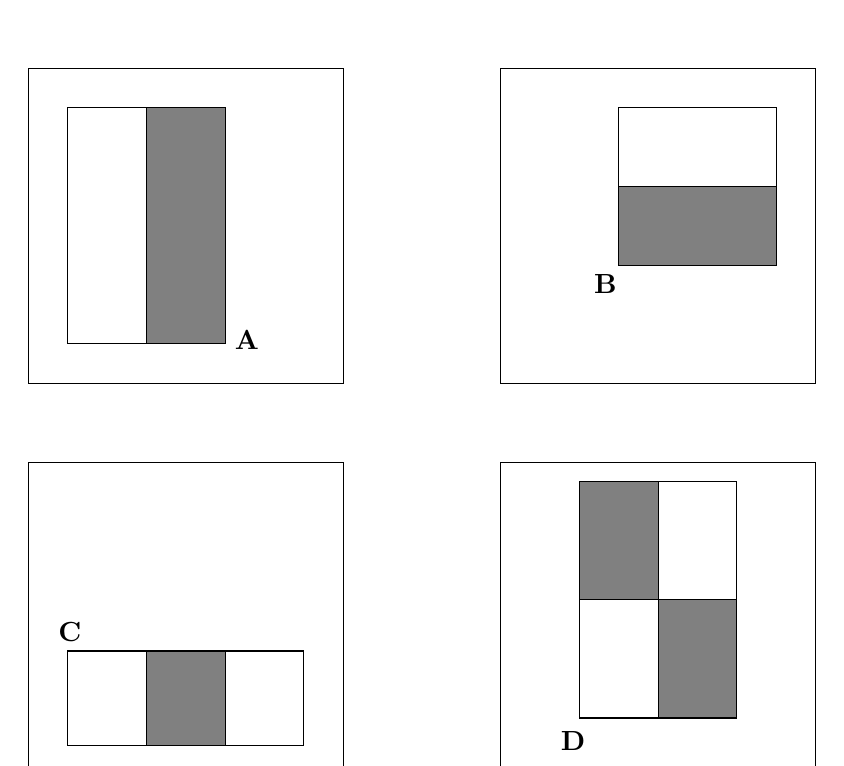
\begin{tikzpicture}
		
		%First square
		\node (firstSquare) at (-3,5) [rectangle, draw, text centered, minimum width=4cm, minimum 
		height=4cm]{};
		
		\node (firstSubSquare1) at (-4,5) [rectangle, draw, text centered, minimum width=1cm, 
		minimum height=3cm]{};
		\node (secondSubSquare1) at (-3,5) [rectangle, draw, text centered, minimum width=1cm, 
		minimum height=3cm, fill=gray]{};
		
		\draw (-2.5, 3.8) coordinate node[below right]{\textbf{A}};
		
		%Second square
		\node (secondSquare) at (3,5) [rectangle, draw, text centered, minimum width=4cm, minimum 
		height=4cm]{};
		
		\node (firstSubSquare2) at (3.5,6) [rectangle, draw, text centered, minimum width=2cm, 
		minimum height=1cm]{};
		\node (secondSubSquare2) at (3.5,5) [rectangle, draw, text centered, minimum width=2cm, 
		minimum height=1cm, fill=gray]{};
		
		\draw (2.6, 4.5) coordinate node[below left]{\textbf{B}};
		
		%Third square
		\node (thirdSquare) at (-3,0) [rectangle, draw, text centered, minimum width=4cm, minimum 
		height=4cm]{};
		
		\node (firstSubSquare3) at (-4,-1) [rectangle, draw, text centered, minimum width=1cm, 
		minimum height=1.2cm]{};
		\node (secondSubSquare3) at (-3,-1) [rectangle, draw, text centered, minimum width=1cm, 
		minimum height=1.2cm, fill=gray]{};
		\node (thirdSubSquare3) at (-2,-1) [rectangle, draw, text centered, minimum width=1cm, 
		minimum height=1.2cm]{};
		
		\draw (-4.2, -0.4) coordinate node[above left]{\textbf{C}};
		
		%Fourth square
		\node (fourthSquare) at (3,0) [rectangle, draw, text centered, minimum width=4cm, minimum 
		height=4cm]{};
		
		\node (firstSubSquare4) at (3.5,1) [rectangle, draw, text centered, minimum width=1cm, 
		minimum height=1.5cm]{};
		\node (secondSubSquare4) at (2.5,1) [rectangle, draw, text centered, minimum width=1cm, 
		minimum height=1.5cm, fill=gray]{};
		\node (thirdSubSquare4) at (3.5,-0.5) [rectangle, draw, text centered, minimum width=1cm, 
		minimum height=1.5cm, fill=gray]{};
		\node (fourthSubSquare4) at (2.5,-0.5) [rectangle, draw, text centered, minimum width=1cm, 
		minimum height=1.5cm]{};
		
		\draw (2.2, -1.3) coordinate node[below left]{\textbf{D}};
		
		\end{tikzpicture}
	}
	\end{center}
	
\end{figure}

\newpage


\section{Example \thevarious}
\stepcounter{various}

\begin{figure}[h]
	\begin{center}
		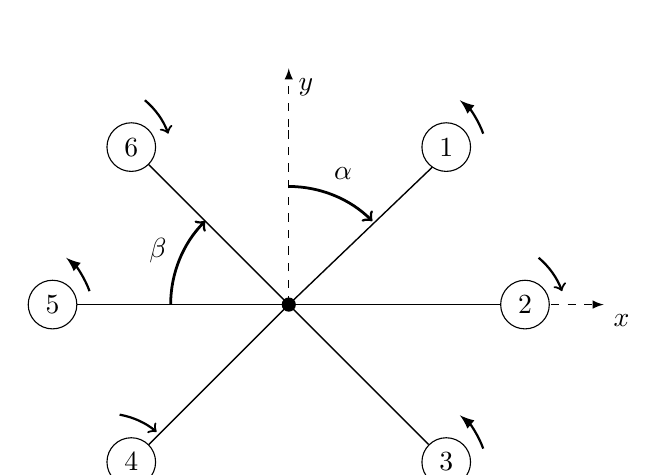
\begin{tikzpicture}
		
		%Reference System
		\draw[-latex, draw, dashed] (3.33,0) coordinate -- (4,0) coordinate node[below right]{$x$};
		\draw[draw, dashed] (0,0) coordinate -- (0,2.25) coordinate;
		\draw[-latex, draw, dashed] (0,2.25) coordinate -- (0,3) coordinate (asse) node[below 
		right]{$y$};
		
		%Circles
		\node[circle,draw,black,minimum size=0.5cm] (A) at (2,2){1};	
		\node[circle,draw,black,minimum size=0.5cm] (B) at (-2,2){6};
		\node[circle,draw,black,minimum size=0.5cm] (C) at (-3,0){5};
		\node[circle,draw,black,minimum size=0.5cm] (D) at (-2,-2){4};
		\node[circle,draw,black,minimum size=0.5cm] (E) at (2,-2){3};
		\node[circle, draw, fill=black, scale=0.5] (center) at (0,0){} pic["$\beta$", draw, <-, 
		angle eccentricity=1.2, angle radius=1.5cm, line width=1.0pt]{angle=B--center--C};
		\node[circle,draw,black,minimum size=0.5cm] (F) at (3,0){2} pic["$\alpha$", draw, <-, angle 
		eccentricity=1.2, angle radius=1.5cm, line width=1.0pt]{angle=A--center--asse};
		
		%Arm links
		\draw[line width=0.5pt] (C.east) -- (F.west);
		\draw[line width=0.5pt] (B.315) -- (0,0) coordinate;
		\draw[line width=0.5pt] (D.45) -- (0,0) coordinate;
		\draw[line width=0.5pt] (E.135) -- (0,0) coordinate;
		\draw[line width=0.5pt] (A.235) -- (0,0) coordinate;
		
		%Angles
		\draw[thick,-latex] ([shift=(20:0.5cm)]2,2) arc (20:50:1cm);
		\draw[thick,-latex] ([shift=(20:0.5cm)]2,-2) arc (20:50:1cm);
		\draw[thick,-latex] ([shift=(20:0.5cm)]-3,0) arc (20:50:1cm);
		\draw[thick,<-] ([shift=(20:0.5cm)]-2,2) arc (20:50:1cm);
		\draw[thick,<-] ([shift=(50:0.5cm)]-2,-2) arc (50:80:1cm);
		\draw[thick,<-] ([shift=(20:0.5cm)]3,0) arc (20:50:1cm);
		
		\end{tikzpicture}
	\end{center}
	
\end{figure}

\section{Example \thevarious}
\stepcounter{various}

\begin{figure}[h]
	\begin{center}
		\begin{tikzpicture}
		
		%Frame
		\node (frame) at (0,0) [rectangle, draw, minimum width=10cm, minimum height=5cm, text 
		centered, label=\textbf{Frame}]{};
		
		%Bounding box
		\node (boundingBox) at (0,0) [rectangle, draw, dashed, minimum width=5cm, minimum 
		height=2cm, text centered, label=\textbf{Bounding Box}]{};
		
		%Vertices coordinates
		\node (verticesCoordinates) at (-2.5,1) [circle, draw, scale=0.4, fill=black]{}; 
		\draw (-2.5,1) coordinate node[above left]{$(x_{vrt},\,y_{vrt})$};
		
		%Curly brackets
		\draw [decorate,decoration={brace,amplitude=10pt,raise=4pt},yshift=0pt]
		(2.5,1) -- (2.5,-1) node [black,midway,xshift=1.1cm] {\footnotesize
			$h_{bb}$};
		
		\draw [decorate,decoration={brace,mirror,amplitude=10pt,raise=4pt},yshift=0pt]
		(-2.5,-1) -- (2.5,-1) node [black,midway,xshift=0cm, yshift=-0.75cm] {\footnotesize
			$w_{bb}$};
		
		
		\end{tikzpicture}
	\end{center}
	
\end{figure}



\section{Example \thevarious}
\stepcounter{various}

\begin{table}[h]
	\centering
	
\begin{tabular}{|M{0.8cm}|M{0.8cm}|M{0.8cm}|M{0.8cm}|M{0.8cm}|M{0.8cm}|M{2cm}|M{1.4cm}|M{1.4cm}|}
		
		\hline
		
		\cellcolor{red}0 & \cellcolor{green}1 & \cellcolor{green}2 & \cellcolor{green}3 & 
		\cellcolor{green}4 & \cellcolor{green}5 & \cellcolor{lightgray}6\,to\,n+6 & 
		\cellcolor{green}n+7 & \cellcolor{green}n+8\\
		
		\hline
		
		str & lgt & seq & cmp & sys & msg & dat & cks & cks\\
		
		\hline
		
	\end{tabular}
	
\end{table}

\newpage


\section{Example \thevarious}
\stepcounter{various}

\begin{figure}[h]
	\begin{center}
		\scalebox{0.8}{
		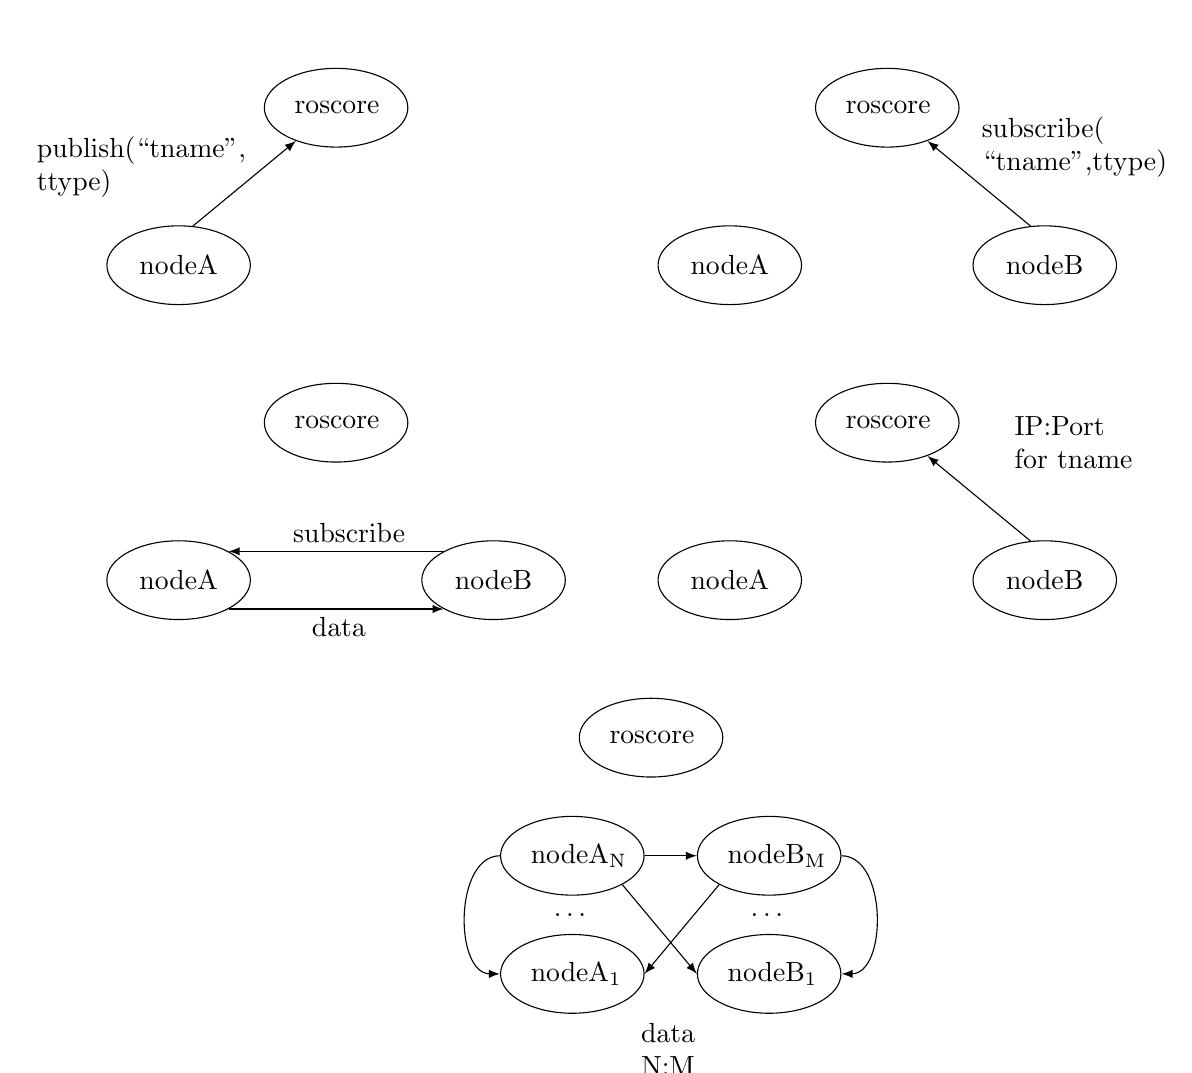
\begin{tikzpicture}
		%First scheme
		\node (roscore1) at (-2,0) [ellipse, draw, text centered, text width=3em, minimum size=1cm] 
		{roscore};
		\node (nodeA1) at (-4,-2) [ellipse, draw, text centered, text width=3em, minimum 
		size=1cm]{nodeA};
		\draw[-latex] (nodeA1.70) -- (roscore1);
		\draw (-5.5,-0.75) coordinate node[left, text width=0.5em]{publish(``tname'',\\ ttype)};
		
		%Second scheme
		\node (roscore2) at (5,0) [ellipse, draw, text centered, text width=3em, minimum size=1cm] 
		{roscore};
		\node (nodeA2) at (3,-2) [ellipse, draw, text centered, text width=3em, minimum 
		size=1cm]{nodeA};
		\node (nodeB2) at (7,-2) [ellipse, draw, text centered, text width=3em, minimum 
		size=1cm]{nodeB};
		\draw[-latex] (nodeB2.110) -- (roscore2);
		\draw (6.5,-0.5) coordinate node[left, text width=0.5em]{subscribe(\\``tname'',ttype)};
		
		%Third scheme
		\node (roscore3) at (5,-4) [ellipse, draw, text centered, text width=3em, minimum size=1cm] 
		{roscore};
		\node (nodeA3) at (3,-6) [ellipse, draw, text centered, text width=3em, minimum 
		size=1cm]{nodeA};
		\node (nodeB3) at (7,-6) [ellipse, draw, text centered, text width=3em, minimum 
		size=1cm]{nodeB};
		\draw[-latex] (nodeB3.110) -- (roscore3);
		\draw (8.5,-4.25) coordinate node[left, text width=5em]{IP:Port\\ for tname};
		
		%Fourth scheme
		\node (roscore4) at (-2,-4) [ellipse, draw, text centered, text width=3em, minimum 
		size=1cm] {roscore};
		\node (nodeA4) at (-4,-6) [ellipse, draw, text centered, text width=3em, minimum 
		size=1cm]{nodeA};
		\node (nodeB4) at (0,-6) [ellipse, draw, text centered, text width=3em, minimum 
		size=1cm]{nodeB};
		\draw[latex-] (nodeA4.30) -- (nodeB4.150);
		\draw (-1,-5.65) coordinate node[above left]{subscribe};
		\draw[-latex] (nodeA4.-30) -- (nodeB4.210);
		\draw (-1.5,-6.35) coordinate node[below left]{data};
		
		%Fifth scheme
		\node (roscore5) at (2,-8) [ellipse, draw, text centered, text width=3em, minimum size=1cm] 
		{roscore};
		\node (nodeAn) at (1,-9.5) [ellipse, draw, text centered, text width=3em, minimum 
		size=1cm]{$\text{nodeA}_\mathrm{N}$};
		\node (nodeBm) at (3.5,-9.5) [ellipse, draw, text centered, text width=3em, minimum 
		size=1cm] {$\text{nodeB}_\mathrm{M}$};
		\node (node) at (1,-10.25) [ellipse, text centered, text width=3em, minimum 
		size=1cm]{\dots};
		\node (node) at (3.5,-10.25) [ellipse, text centered, text width=3em, minimum size=1cm] 
		{\dots};
		\node (nodeA11) at (1,-11) [ellipse, draw, text centered, text width=3em, minimum 
		size=1cm]{$\text{nodeA}_\mathrm{1}$};
		\node (nodeB11) at (3.5,-11) [ellipse, draw, text centered, text width=3em, minimum 
		size=1cm] {$\text{nodeB}_\mathrm{1}$};
		\draw[-latex] (nodeAn.0) -- (nodeBm.180);
		\draw[latex-] (nodeA11.0) -- (nodeBm.210);
		\draw[-latex] (nodeAn.-30) -- (nodeB11.180);
		\draw[latex-] (nodeB11) to [out=0,in=0] (nodeBm);
		\draw[latex-] (nodeA11) to [out=180,in=180] (nodeAn);
		\draw (2.4,-11.5) coordinate node[below, text width=3em]{data N:M};
		
		\end{tikzpicture}
	}
	\end{center}

\end{figure}


\section{Example \thevarious}
\stepcounter{various}

\begin{figure}[h]
	\begin{center}
		\scalebox{0.8}{
		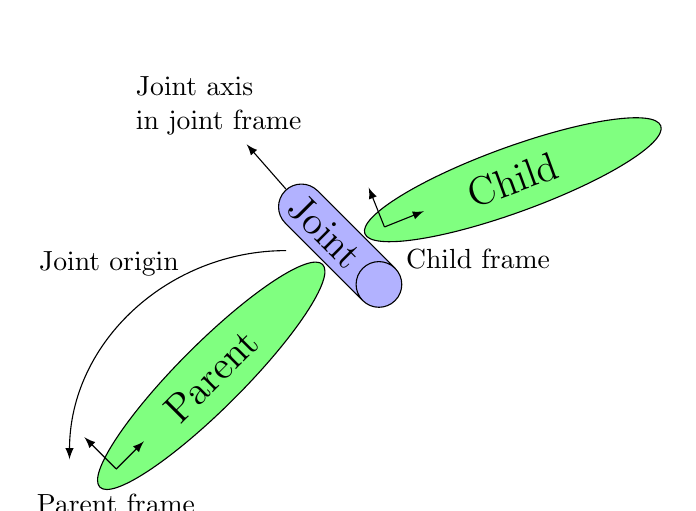
\begin{tikzpicture}
		%Shapes
		\node (ellisse1) at (-0.7,-0.44) [draw, ellipse, text centered, rotate=45, fill=green!50, 
		minimum width=4cm]{\Large{Parent}};
		\node (ellipse2) at (3.13,2.05) [draw, ellipse, text centered, rotate=20, fill=green!50, 
		minimum width=4cm]{\Large{Child}};
		\node (cilindro) at (0.75,1.4) [draw, cylinder, text centered, rotate=-45, 
		fill=blue!30]{\Large{Joint}};
		
		%Axes
		\draw[-latex, rotate=-45] (-0.2,-2.5) coordinate -- (-0.2,-2) coordinate;
		\draw[-latex] (-1.91,-1.62) coordinate node at(-1.91,-1.82) [below]{Parent frame} -- 
		(-2.31,-1.22) coordinate;
		
		\draw[-latex] (1.5,1.45) coordinate -- (1.3,1.95) coordinate node at (1.65,1.05) 
		[right]{Child frame};
		\draw[-latex] (1.5,1.45) coordinate -- (2,1.65) coordinate;
		\draw[-latex] (0.25,1.93) coordinate -- (-0.25,2.5) coordinate node[above, text 
		width=8em]{Joint axis\\in joint frame};
		
		\draw[-latex] (0.25,1.15) [out=180, in=90] to (-2.5,-1.5) node at(-2,0.7) [above]{Joint 
		origin};
		\end{tikzpicture}
	}
	\end{center}

\end{figure}

\newpage

\section{Example \thevarious}
\stepcounter{various}

\begin{figure}[h]
	\begin{center}
		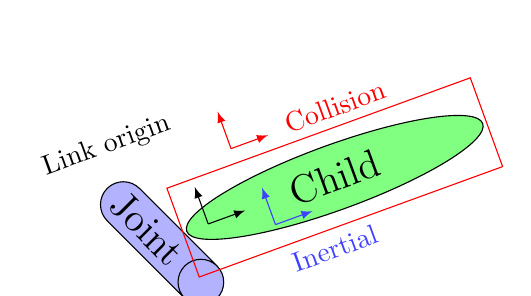
\begin{tikzpicture}
		\node (ellipse2) at (3.13,2.05) [draw, ellipse, text centered, rotate=20, fill=green!50, 
		minimum width=4cm]{\Large{Child}};
		\node (cilindro) at (0.75,1.4) [draw, cylinder, text centered, rotate=-45, 
		fill=blue!30]{\Large{Joint}};
		\node (collision) at (3.13,2.05) [draw=red, rectangle, minimum width=4.1cm, minimum 
		height=1.2cm, rotate=20]{};
		
		\draw[draw] node at (3.13,2.95)[text centered, rotate=20]{\textcolor{red}{Collision}};
		\draw[draw] node at (3.13,1.15)[text centered, rotate=20]{\textcolor{blue!75}{Inertial}};
		\draw[draw] node at (0.23,2.45)[text centered, rotate=20]{Link origin};
		
		%Link Collision
		\draw[-latex, rotate=20, red] (2.53,1.65) coordinate -- (3.03,1.65) coordinate;
		\draw[-latex, rotate=20, red] (2.53,1.65) coordinate -- (2.53,2.15) coordinate;
		
		\draw[-latex, rotate=20, blue!75] (2.73,0.55) coordinate -- (3.23,0.55) coordinate;
		\draw[-latex, rotate=20, blue!75] (2.73,0.55) coordinate -- (2.73,1.05) coordinate;
		
		\draw[-latex, rotate=20] (1.93,0.85) coordinate -- (2.43,0.85) coordinate;
		\draw[-latex, rotate=20] (1.93,0.85) coordinate -- (1.93,1.35) coordinate;
		\end{tikzpicture}
	\end{center}

\end{figure}


\section{Example \thevarious}
\stepcounter{various}

\begin{figure}[h]
	\begin{center}
		\scalebox{0.8}{
		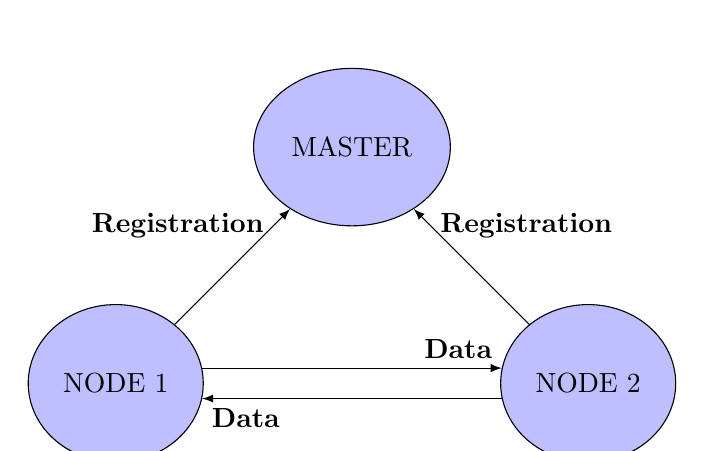
\begin{tikzpicture}
		%Nodes of the net
		\node (master) at (0,0) [draw, ellipse, minimum width=2cm, minimum height=2cm, text 
		centered, fill=blue!25]{MASTER};
		\node (node2) at (3,-3) [draw, ellipse, minimum width=2cm, minimum height=2cm, text 
		centered, fill=blue!25]{NODE 2};
		\node (node1) at (-3,-3) [draw, ellipse, minimum width=2cm, minimum height=2cm, text 
		centered, fill=blue!25]{NODE 1};
		
		%Links among nodes
		\draw[-latex] (node1.10) -- (node2.170) node[above left]{\textbf{Data}};
		\draw[-latex] (node2.190) -- (node1.350) node[below right]{\textbf{Data}};
		\draw[-latex] (node1) -- (master) node at (-1,-1) [left]{\textbf{Registration}};
		\draw[-latex] (node2) -- (master) node at (1,-1) [right]{\textbf{Registration}};
		\end{tikzpicture}
	}
	\end{center}
	
\end{figure}

\section{Example \thevarious}
\stepcounter{various}

\begin{figure}[h]
	\begin{center}
		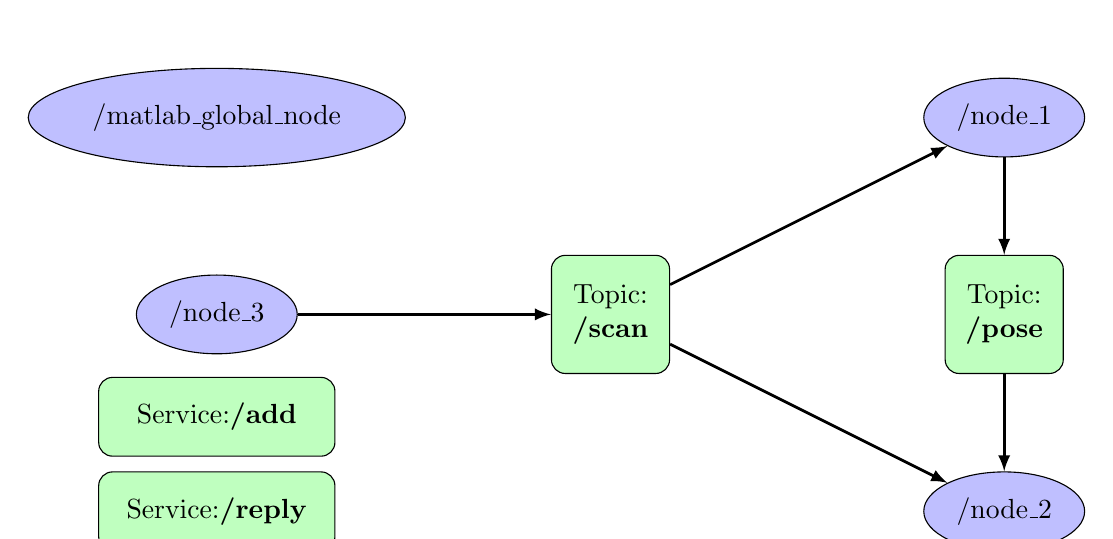
\begin{tikzpicture}
		%Nodes of the net
		\node (matlab) at (0,0) [draw, ellipse, minimum height=1.25cm, minimum width=0.5cm, text 
		centered, fill=blue!25]{/matlab\_global\_node};
		\node (node1) at (10,0) [draw, ellipse, minimum size=1cm, text centered, 
		fill=blue!25]{/node\_1};
		\node (node2) at (10,-5) [draw, ellipse, minimum size=1cm, text centered, 
		fill=blue!25]{/node\_2};
		\node (node3) at (0,-2.5) [draw, ellipse, minimum size=1cm, text centered, 
		fill=blue!25]{/node\_3};
		
		%Topics of the net
		\node (topicPose) at (10,-2.5) [draw, rectangle, minimum size=1.5cm, text centered, 
		fill=green!25, text width=3em, rounded corners=5pt]{Topic:\\\textbf{/pose}}; 
		\node (topicScan) at (5,-2.5) [draw, rectangle, minimum size=1.5cm, text centered, 
		fill=green!25, text width=3em, rounded corners=5pt]{Topic:\\\textbf{/scan}};
		
		%Services of the net
		\node (serviceAdd) at (0,-3.8) [draw, rectangle, minimum height=1cm, text centered, 
		fill=green!25, minimum width=3cm, rounded corners=5pt]{Service:\textbf{/add}};
		\node (serviceReply) at (0,-5) [draw, rectangle, minimum height=1cm, minimum width=3cm, 
		text centered, fill=green!25, rounded corners=5pt]{Service:\textbf{/reply}};
		
		%Links between topics and services
		\draw[-latex, line width=1pt] (topicScan) -- (node1);
		\draw[-latex, line width=1pt] (node1) -- (topicPose);
		\draw[-latex, line width=1pt] (topicPose) -- (node2);
		\draw[-latex, line width=1pt] (node3) -- (topicScan);
		\draw[-latex, line width=1pt] (topicScan) -- (node2);
		\end{tikzpicture}
	\end{center}
	
\end{figure}

\newpage

\section{Example \thevarious}
\stepcounter{various}

\begin{figure}[h]
	\begin{center}
		\scalebox{0.9}{
		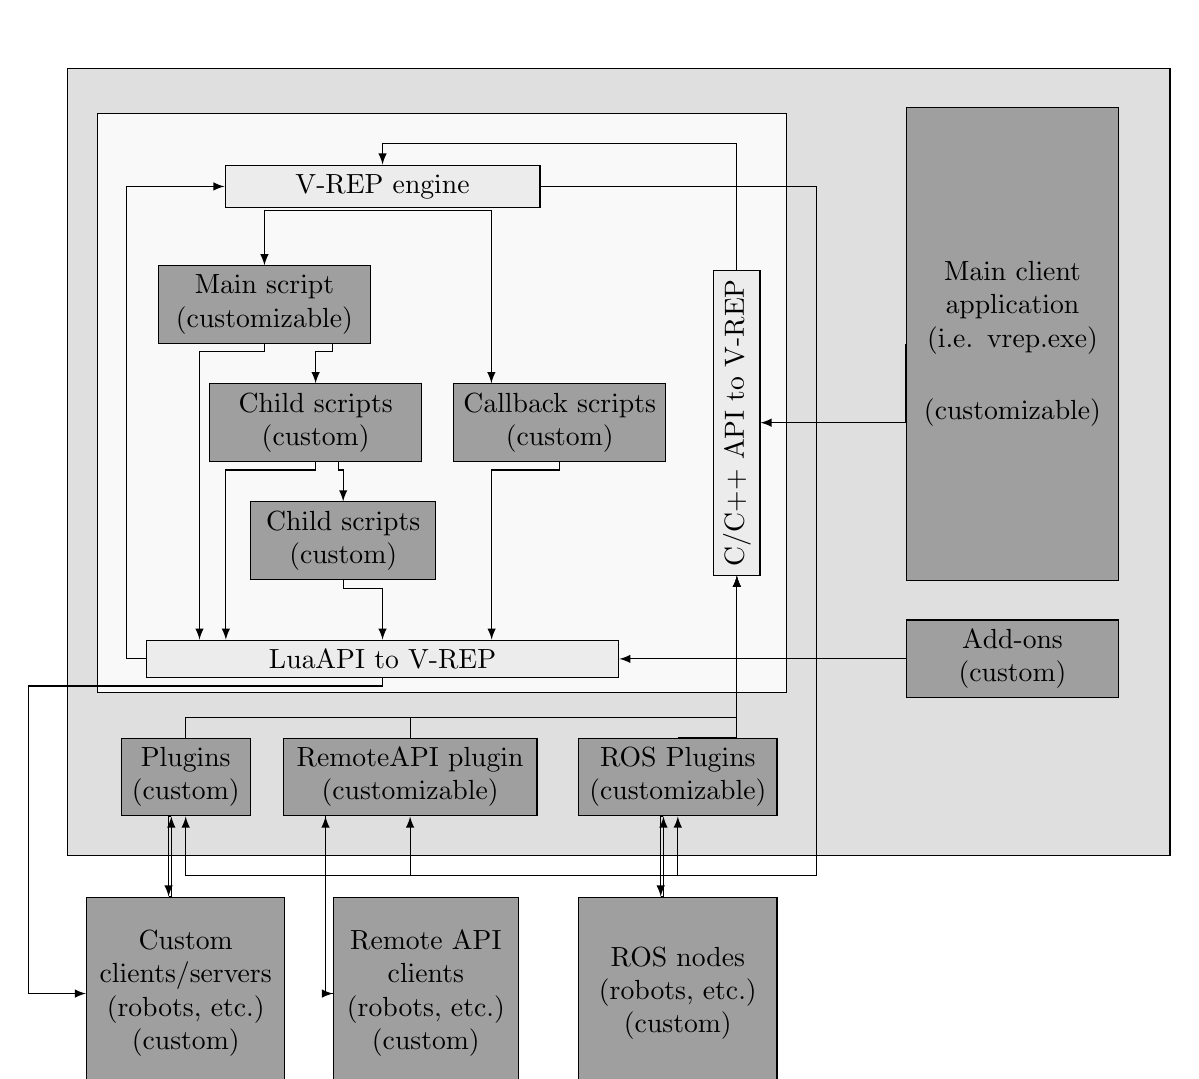
\begin{tikzpicture}
		\node (frameWork) at (0,0) [draw, rectangle, minimum width=14cm, minimum height=10cm, text 
		centered, fill=gray!25]{};
		
		\node (shareLibrary) at (-2.25,0.75) [draw, rectangle, minimum width=8.75cm, minimum 
		height=7.35cm, text centered, fill=gray!5]{};
		
		\node (V-REP engine) at (-3,3.5) [draw, rectangle, text centered, minimum width=4cm, 
		fill=gray!15]{V-REP engine};
		
		\node (Main Script) at (-4.5,2) [draw, rectangle, text centered, text width=7em, 
		fill=gray!75]{Main script\\(customizable)};
		
		\node (Child Script) at (-3.85,0.5) [draw, rectangle, text centered, text width=7em, 
		fill=gray!75]{Child scripts\\(custom)};
		
		\node (Callback Script) at (-0.75,0.5) [draw, rectangle, text centered, text width=7em, 
		fill=gray!75]{Callback scripts\\(custom)};
		
		\node (C/C++ API to V-REP) at (1.5,0.5) [draw, rectangle, rotate=90, text centered, 
		fill=gray!15]{C/C++ API to V-REP};
		
		\node (Child scripts2) at (-3.5,-1) [draw, rectangle, text centered, text width=6em, 
		fill=gray!75]{Child scripts\\(custom)};
		
		\node (LuaAPI) at (-3,-2.5) [draw, rectangle, text centered, minimum width=6cm, 
		fill=gray!15]{LuaAPI to V-REP};
		
		\node (Plugins) at (-5.5,-4) [draw, rectangle, text centered, text width=4em, 
		fill=gray!75]{Plugins\\(custom)};
		
		\node (RemoteAPI Plugins) at (-2.65,-4) [draw, rectangle, text centered, text width=8.5em, 
		fill=gray!75]{RemoteAPI plugin\\(customizable)};
		
		\node (ROS Plugins) at (0.75,-4) [draw, rectangle, text centered, text width=6.5em, 
		fill=gray!75]{ROS Plugins\\(customizable)};
		
		\node (Custom) at (-5.5,-6.75) [text centered, draw, rectangle, text width=6.5em, minimum 
		height=2.45cm, fill=gray!75]{Custom\\clients/servers\\(robots, etc.)\\(custom)};
		
		\node (Remote) at (-2.45,-6.75) [text centered, draw, rectangle, text width=6em, minimum 
		height=2.45cm, fill=gray!75]{Remote API\\clients\\(robots, etc.)\\(custom)};
		
		\node (ROSnodes) at (0.75,-6.75) [text centered, draw, rectangle, text width=6.5em, minimum 
		height=2.45cm, fill=gray!75]{ROS nodes\\(robots, etc.)\\(custom)};
		
		\node (Add-ons) at (5,-2.5) [draw, rectangle, text centered, text width=7em, 
		fill=gray!75]{Add-ons\\(custom)};
		
		\node (Main client) at (5,1.5) [draw, minimum height=6cm, rectangle, text centered, text 
		width=7em, fill=gray!75]{Main client\\application\\(i.e. 
		vrep.exe)\\\vspace{0.5cm}(customizable)};
		
		%Links
		\draw[-latex] (V-REP engine) ++(0,-0.3) -| (Main Script.90);
		\draw[-latex] (V-REP engine) ++(0,-0.3) -| (Callback Script.150);
		\draw[-latex] (V-REP engine.0) ++(0,0) -| ++(3.5,0) |- ++(0,-8.75) |- ++(0,0) -| (ROS 
		Plugins.270);
		\draw[-latex] (V-REP engine.0) ++(0,0) -| ++(3.5,0) |- ++(0,-8.75) |- ++(0,0) -| 
		(Plugins.270);
		\draw[-latex] (V-REP engine.0) ++(0,0) -| ++(3.5,0) |- ++(0,-8.75) |- ++(0,0) -| (RemoteAPI 
		Plugins.270);
		\draw[-latex] (LuaAPI.180) -| ++(-0.25,0) -| ++(0,0) |- (V-REP engine.180);
		\draw[-latex] (Main Script.330) ++(0,0) -| ++(0,-0.1) -| (Child Script.90);
		\draw[-latex] (Main Script.270) ++(0,0) -| ++(0,-0.1) -| (LuaAPI.174);
		\draw[-latex] (Child Script.270) ++(0,0) -| ++(0,-0.1) -| (LuaAPI.173);
		\draw[-latex] (Child Script.300) ++(0,0) -| ++(0,-0.1) -| (Child scripts2.90);
		\draw[-latex] (Child scripts2.270) ++(0,0) -| ++(0,-0.1) -| (LuaAPI.90);
		\draw[-latex] (Callback Script.270) ++(0,0) -| ++(0,-0.1) -| (LuaAPI.10);
		\draw[-latex] (Add-ons) -- (LuaAPI.0);
		\draw[-latex] (C/C++ API to V-REP.0) ++(0,0) |- ++(0,1.6) -| (V-REP engine.90);
		\draw[-latex] (Main client.180) ++(0,0) |- (C/C++ API to V-REP.270);
		\draw[-latex] (ROS Plugins.90) ++(0,0) -| ++(0,0) |- ++(0,0) |- ++(0,0) -| (C/C++ API to 
		V-REP.180);
		\draw[-latex] (RemoteAPI Plugins.90) ++(0,0) -| ++(0,0.25) |- ++(0,0) -| (C/C++ API to 
		V-REP.180);
		\draw[-latex] (Plugins.90) ++(0,0) -| ++(0,0.25) |- ++(0,0) -| (C/C++ API to V-REP.180);
		\draw[-latex] (ROSnodes.100) -| (ROS Plugins.250);
		\draw[latex-] (ROSnodes.100) |- (ROS Plugins.250);
		\draw[-latex] (Custom.100) -| (Plugins.250);
		\draw[latex-] (Custom.100) |- (Plugins.250);
		\draw[-latex] (LuaAPI.270) ++(0,0) -| ++(0,-0.1) |- ++(0,0) |- ++(-4.5,0) -| ++(0,0) |- 
		(Custom.180);
		\draw[-latex] (Remote.180) ++(0,0) |- ++(-0.1,0) -| (RemoteAPI Plugins.205);  
		\draw[-latex] (RemoteAPI Plugins.205) ++(0,0) |- (Remote.180);
		
		\end{tikzpicture}
	}
	\end{center}

\end{figure}

\section{Example \thevarious}
\stepcounter{various}

\begin{figure}[h]
	\centering
	\scalebox{0.4}{
		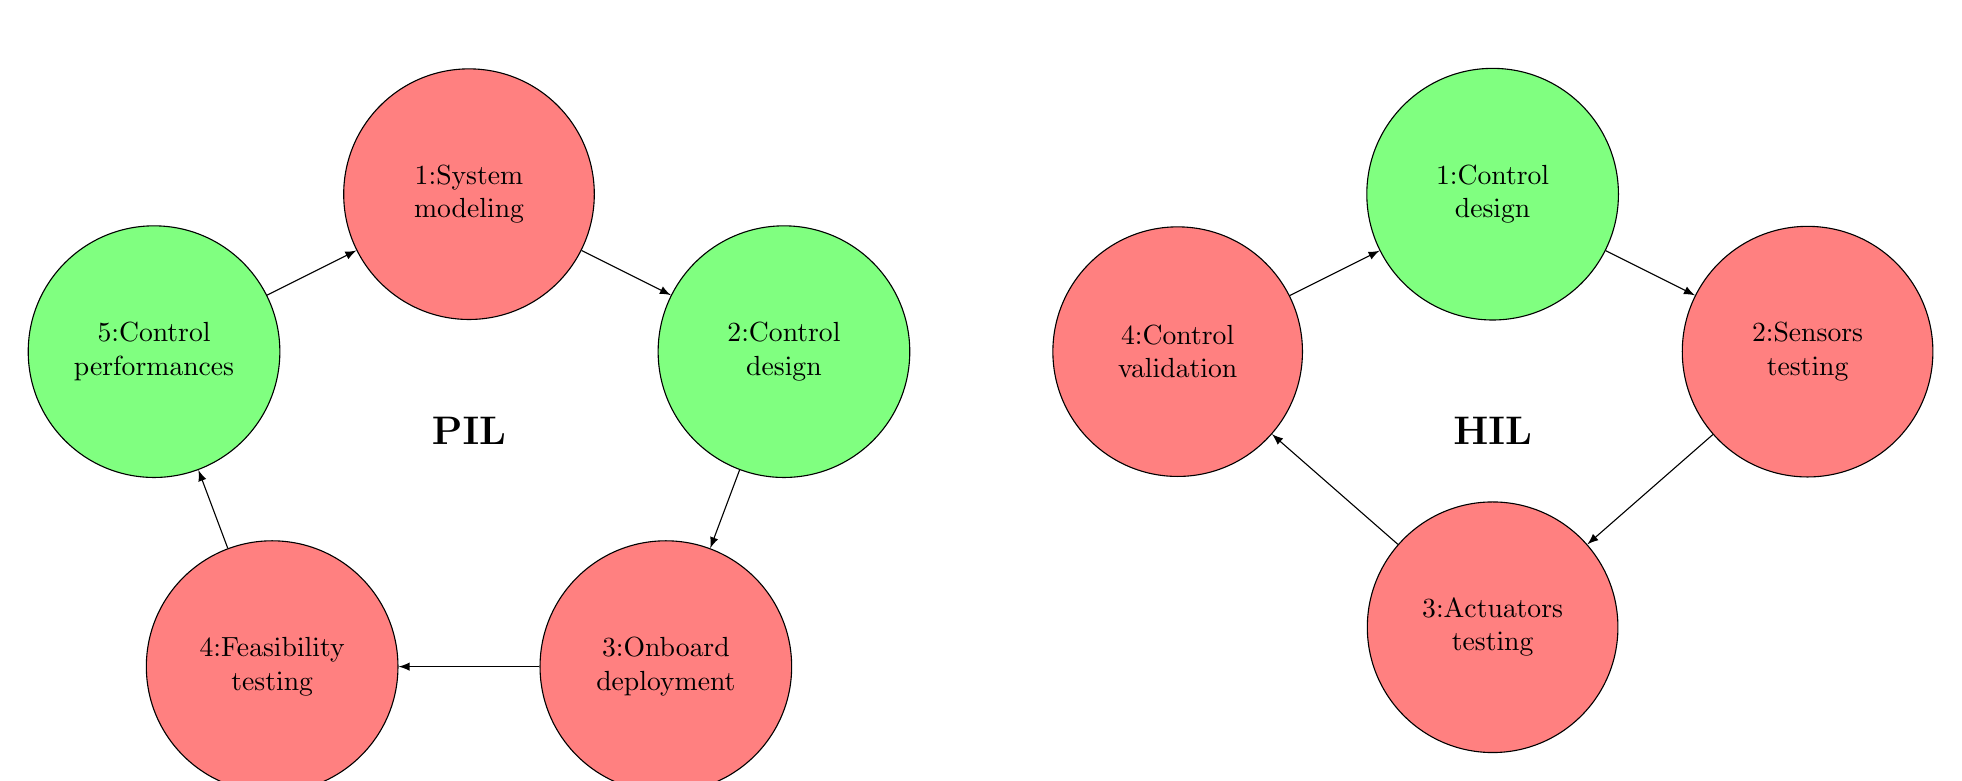
\begin{tikzpicture}
		%PIL's nodes
		\node (System Modeling) at (0,1) [circle, draw, minimum size=1cm, text centered, text 
		width=8em, fill=red!50]{1:System \\ modeling};
		\node (Control Design) at (4,-1) [circle, draw, minimum size=1cm, text centered, text 
		width=8em, fill=green!50]{2:Control \\ design};
		\node (Board Deploy) at (2.5,-5) [circle, draw, minimum size=1cm, text centered, text 
		width=8em, fill=red!50]{3:Onboard \\ deployment};
		
		\node (Feasibility Testing) at (-2.5,-5) [circle, draw, minimum size=1cm, text centered, 
		text width=8em, fill=red!50]{4:Feasibility \\ testing};
		\node (Control Performance) at (-4,-1) [circle, draw, minimum size=1cm, text centered, text 
		width=8em, fill=green!50]{5:Control \\ performances};
		
		\node (PIL) at (0,-2) [text centered]{\textbf{\Large{PIL}}};
		
		%PIL links
		\draw[-latex] (System Modeling) -- (Control Design);
		\draw[-latex] (Control Design) -- (Board Deploy);
		\draw[-latex] (Board Deploy) -- (Feasibility Testing);
		\draw[-latex] (Feasibility Testing) -- (Control Performance);
		\draw[-latex] (Control Performance) -- (System Modeling);
		
		%HIL's nodes
		\node (Control Design 1) at (13,1) [circle, draw, minimum size=1cm, text centered, text 
		width=8em, fill=green!50]{1:Control \\ design};
		\node (Sensor Testing) at (17,-1) [circle, draw, minimum size=1cm, text centered,  text 
		width=8em, fill=red!50]{2:Sensors \\ testing};
		\node (Actuators Testing) at (13,-4.5) [circle, draw, minimum size=1cm, text centered,  
		text width=8em, fill=red!50]{3:Actuators \\testing};
		\node (Control Validation) at (9,-1) [circle, draw, minimum size=1cm, text centered, text 
		width=8em, fill=red!50]{4:Control \\validation};
		
		\node (HIL) at (13,-2) [text centered]{\textbf{\Large{HIL}}};
		
		%HIL links
		\draw[-latex] (Control Design 1) -- (Sensor Testing);
		\draw[-latex] (Sensor Testing) -- (Actuators Testing);
		\draw[-latex] (Actuators Testing) -- (Control Validation);
		\draw[-latex] (Control Validation) -- (Control Design 1);
		
		\end{tikzpicture}
	}

\end{figure}

\newpage

\section{Example \thevarious}
\stepcounter{various}

\begin{figure}[h]
	\centering
	\subfigure[]{
		\scalebox{0.8}{
		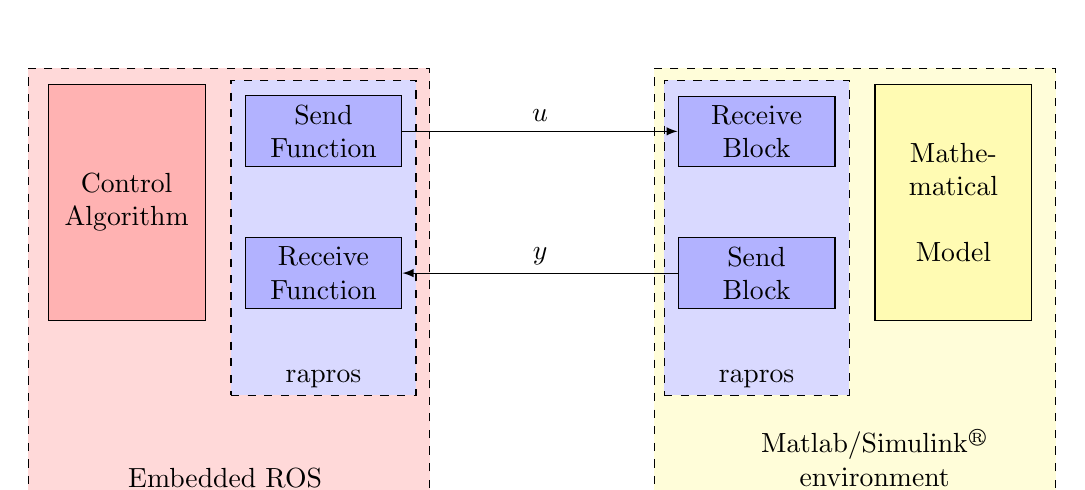
\begin{tikzpicture}
		%First block's components
		\node (Embedded ROS) at (0.05,-1.05) [draw, rectangle, dashed, minimum height=5.5cm, 
		minimum width=5.1cm, text centered, fill=red!15]{};
		\node (Control Algorithm) at (-1.25,0) [draw, rectangle, minimum height=3cm, minimum 
		width=1cm, text centered, text width=5em, fill=red!30]{Control \\Algorithm};
		\node (wrapper1) at (1.25,-0.45) [draw, rectangle, dashed, minimum height=4cm, minimum 
		width=2.35cm, text centered, fill=blue!15]{};
		\node (Send Function) at (1.25,0.9) [draw, rectangle, minimum height=0.5cm, minimum 
		width=1cm, text centered, text width=5em, fill=blue!30]{Send \\Function};
		\node (Receive Function) at (1.25,-0.9) [draw, rectangle, minimum height=0.5cm, minimum 
		width=1cm, text centered, text width=5em, fill=blue!30]{Receive \\Function};
		
		%Writing inside the first block
		\node (Scritto1) at (0,-3.5) [text centered]{Embedded ROS};
		\node (Scritto2) at (1.25,-2.25) [text centered]{rapros};
		
		%Second block's components
		\node (Embedded ROS) at (8,-1.05) [draw, rectangle, dashed, minimum height=5.5cm, minimum 
		width=5.1cm, text centered, fill=yellow!15]{};
		\node (Mathematical Model) at (9.25,0) [draw, rectangle, minimum height=3cm, minimum 
		width=1cm, text centered, text width=5em, fill=yellow!30]{Mathe-\\matical\\~\\Model};
		\node (wrapper1) at (6.75,-0.45) [draw, rectangle, dashed, minimum height=4cm, minimum 
		width=2.35cm, text centered, fill=blue!15]{};
		\node (Receive Block) at (6.75,0.9) [draw, rectangle, minimum height=0.5cm, minimum 
		width=1cm, text centered, text width=5em, fill=blue!30]{Receive \\Block};
		\node (Send Block) at (6.75,-0.9) [draw, rectangle, minimum height=0.5cm, minimum 
		width=1cm, text centered, text width=5em, fill=blue!30]{Send \\Block};
		
		%Writing inside the second block
		\node (Scritto1) at (8.25,-3.25) [text centered, text 
		width=9em]{Matlab/Simulink\textsuperscript{\circledR} \\environment};
		\node (Scritto2) at (6.75,-2.25) [text centered]{rapros};
		
		%Links amonb blocks
		\draw[-latex] (Send Function.0) -- (Receive Block.180) node at(4,1.3) [below]{$u$};
		\draw[-latex] (Send Block.180) -- (Receive Function.0) node at(4,-0.45) [below]{$y$};
		
		\end{tikzpicture}
	}
		
	}
	\subfigure[]{
		\scalebox{0.8}{
		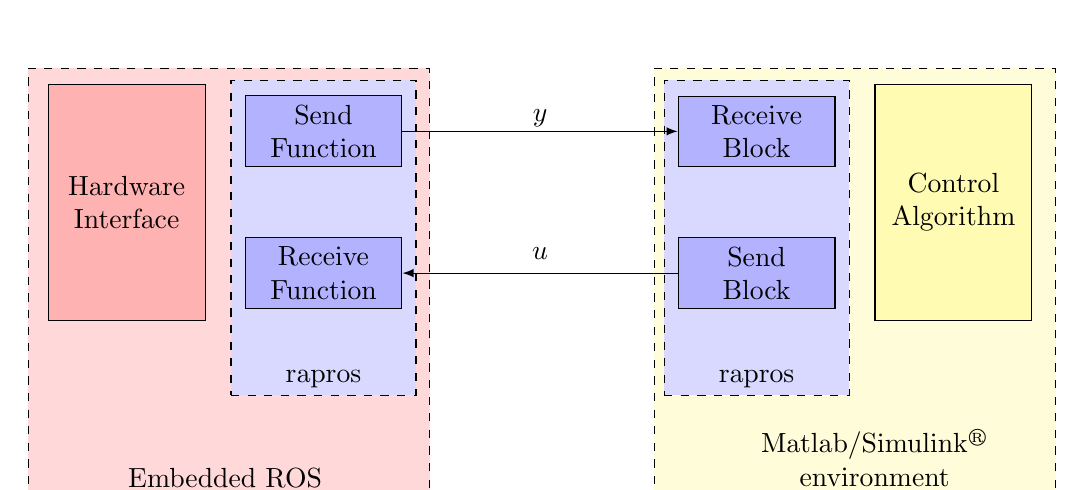
\begin{tikzpicture}
		\node (Embedded ROS) at (0.05,-1.05) [draw, rectangle, dashed, minimum height=5.5cm, 
		minimum width=5.1cm, text centered, fill=red!15]{};
		\node (Hardware Interface) at (-1.25,0) [draw, rectangle, minimum height=3cm, minimum 
		width=1cm, text centered, text width=5em, fill=red!30]{Hardware \\Interface};
		\node (wrapper1) at (1.25,-0.45) [draw, rectangle, dashed, minimum height=4cm, minimum 
		width=2.35cm, text centered, fill=blue!15]{};
		\node (Send Function) at (1.25,0.9) [draw, rectangle, minimum height=0.5cm, minimum 
		width=1cm, text centered, text width=5em, fill=blue!30]{Send \\Function};
		\node (Receive Function) at (1.25,-0.9) [draw, rectangle, minimum height=0.5cm, minimum 
		width=1cm, text centered, text width=5em, fill=blue!30]{Receive \\Function};
		
		\node (Scritto1) at (0,-3.5) [text centered]{Embedded ROS};
		\node (Scritto2) at (1.25,-2.25) [text centered]{rapros};
		
		\node (Embedded ROS) at (8,-1.05) [draw, rectangle, dashed, minimum height=5.5cm, minimum 
		width=5.1cm, text centered, fill=yellow!15]{};
		\node (Control Algorithm) at (9.25,0) [draw, rectangle, minimum height=3cm, minimum 
		width=1cm, text centered, text width=5em, fill=yellow!30]{Control\\Algorithm};
		\node (wrapper1) at (6.75,-0.45) [draw, rectangle, dashed, minimum height=4cm, minimum 
		width=2.35cm, text centered, fill=blue!15]{};
		\node (Receive Block) at (6.75,0.9) [draw, rectangle, minimum height=0.5cm, minimum 
		width=1cm, text centered, text width=5em, fill=blue!30]{Receive \\Block};
		\node (Send Block) at (6.75,-0.9) [draw, rectangle, minimum height=0.5cm, minimum 
		width=1cm, text centered, text width=5em, fill=blue!30]{Send \\Block};
		
		\node (Scritto1) at (8.25,-3.25) [text centered, text 
		width=9em]{Matlab/Simulink\textsuperscript{\circledR} \\environment};
		\node (Scritto2) at (6.75,-2.25) [text centered]{rapros};
		
		\draw[-latex] (Send Function.0) -- (Receive Block.180) node at(4,1.3) [below]{$y$};
		\draw[-latex] (Send Block.180) -- (Receive Function.0) node at(4,-0.45) [below]{$u$};
		\end{tikzpicture}
	}
		
	}

\end{figure}


\section{Example \thevarious}
\stepcounter{various}


\begin{figure}[h]
	\begin{center}
		\scalebox{0.8}{
		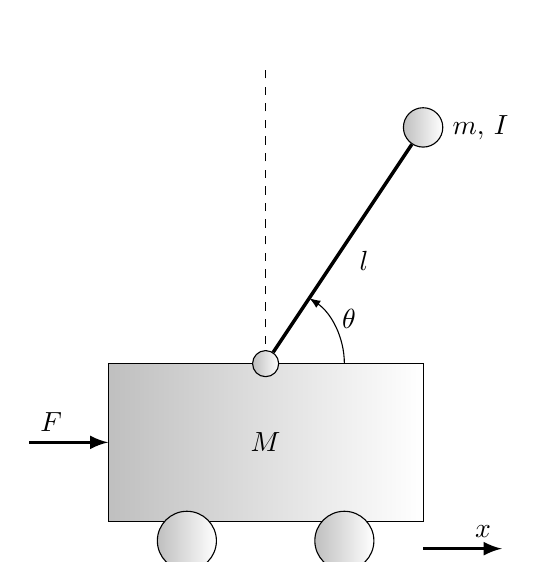
\begin{tikzpicture}
		
		%Reference system
		\draw[dashed] (-2,-2.75) coordinate -- (-2,0.75) coordinate;
		\draw[dashed] (-2,-3.25) coordinate -- (-2,-3.5) coordinate;
		
		%First sphere
		\node (firstSphere) at(0,0) [draw, circle, minimum size=0.5cm, text centered, left 
		color=gray!50, right color=white, shading = axis]{};
		\draw (0.25,0) node[right]{$m,\,I$};
		
		%Body
		\filldraw[left color=gray!50, right color=white, shading = axis] (-4,-3) rectangle (0,-5);
		
		%Second sphere
		\node (secondSphere) at(-2,-3) [draw, circle, left color=gray!50, right color=white, 
		shading = axis, minimum size=0.15cm, text centered]{};
		
		%Links
		\draw[line width=1.25pt] (firstSphere) -- (secondSphere);
		\draw (-0.75,-1.7) node{$l$};
		
		%Arrow
		\draw[-latex, line width=1.25pt] (-5,-4) node[above right]{$F$} -- (-4,-4);
		
		%Angle
		\draw[] (secondSphere) -- (0,-3) coordinate (c);
		\draw pic["$\mathbf{\theta}$", draw, -latex, angle eccentricity=1.2, angle 
		radius=1cm]{angle=c--secondSphere--firstSphere};
		
		%Wheels
		\node (firstWheel) at(-3,-5.25) [draw, circle, left color=gray!50, right color=white, 
		shading = axis, minimum size=0.75cm, text centered]{};
		\node (secondWheel) at(-1,-5.25) [draw, circle, left color=gray!50, right color=white, 
		shading = axis, minimum size=0.75cm, text centered]{};
		
		%Baseline
		\draw[line width=1.25pt] (-5,-5.65) coordinate -- (1,-5.65) coordinate;
		
		%x
		\draw[-latex, line width=1.25pt] (0,-5.35) coordinate -- (1,-5.35) coordinate node[above 
		left]{$x$};
		
		%body mass
		\draw (-2,-3.75) coordinate node[below]{$M$};
		
		\end{tikzpicture}
	}
	\end{center}
\end{figure}

\newpage


\section{Example \thevarious}
\stepcounter{various}

\begin{figure}[h]
	\begin{center}
		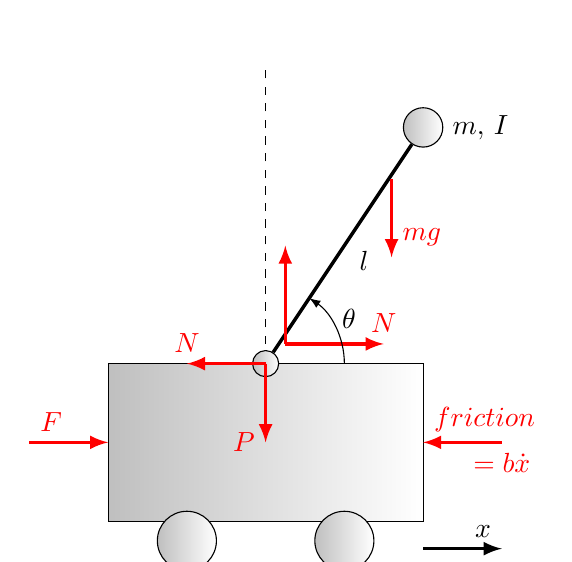
\begin{tikzpicture}
		
		%Reference system
		\draw[dashed] (-2,-2.75) coordinate -- (-2,0.75) coordinate;
		\draw[dashed] (-2,-3.25) coordinate -- (-2,-3.5) coordinate;
		
		%First sphere
		\node (firstSphere) at(0,0) [draw, circle, minimum size=0.5cm, text centered, left 
		color=gray!50, right color=white, shading = axis]{};
		\draw (0.25,0) node[right]{$m,\,I$};
		
		%Body
		\filldraw[left color=gray!50, right color=white, shading = axis] (-4,-3) rectangle (0,-5);
		
		%Second sphere
		\node (secondSphere) at(-2,-3) [draw, circle, left color=gray!50, right color=white, 
		shading = axis, minimum size=0.15cm, text centered]{};
		
		%Links
		\draw[line width=1.25pt] (firstSphere) -- (secondSphere);
		\draw (-0.75,-1.7) node{$l$};
		
		%Arrow
		\draw[-latex, red, line width=1.25pt] (-5,-4) node[above right]{$F$} -- (-4,-4);
		
		%Frction force
		\draw[latex-, red, line width=1.25pt] (0,-4) coordinate node[above right]{$friction$} -- 
		(1,-4) coordinate node[below]{$=b\dot{x}$};
		
		%Forces
		\draw[-latex, red, line width=1.25pt] (-2,-3) coordinate -- (-2,-4) coordinate 
		node[left]{$P$};
		\draw[-latex, red, line width=1.25pt] (-2,-3) coordinate -- (-3,-3) coordinate 
		node[above]{$N$};
		
		\draw[-latex, red, line width=1.25pt] (-1.75,-2.75) coordinate -- (-1.75,-1.5) coordinate;
		\draw[-latex, red, line width=1.25pt] (-1.75,-2.75) coordinate -- (-0.5,-2.75) coordinate 
		node[above]{$N$};
		
		\draw[-latex, red, line width=1.25pt] (-0.4,-0.65) coordinate -- (-0.4,-1.65) coordinate 
		node[above right]{$mg$};
		
		%Angle
		\draw[] (secondSphere) -- (0,-3) coordinate (c);
		\draw pic["$\mathbf{\theta}$", draw, -latex, angle eccentricity=1.2, angle 
		radius=1cm]{angle=c--secondSphere--firstSphere};
		
		%Wheels
		\node (firstWheel) at(-3,-5.25) [draw, circle, left color=gray!50, right color=white, 
		shading = axis, minimum size=0.75cm, text centered]{};
		\node (secondWheel) at(-1,-5.25) [draw, circle, left color=gray!50, right color=white, 
		shading = axis, minimum size=0.75cm, text centered]{};
		
		%Baseline
		\draw[line width=1.25pt] (-5,-5.65) coordinate -- (1,-5.65) coordinate;
		
		%X
		\draw[-latex, line width=1.25pt] (0,-5.35) coordinate -- (1,-5.35) coordinate node[above 
		left]{$x$};
		
		\end{tikzpicture}
	\end{center}

\end{figure}


\section{Example \thevarious}
\stepcounter{various}

\begin{figure}[h]
	\begin{center}
		\begin{tikzpicture}
		
		%Virtual reference system 
		\draw[latex-] (0.4,2) [draw=green] arc (0:-90:1.2cm) node[anchor=south]{$\phi$};
		
		\draw[latex-] (2.7,0.6) [draw=yellow] arc (0:-130:1cm)  node[anchor=north]{$\psi$};
		
		\draw[latex-] (-0.6,-0.7) [draw=red] arc (0:-140:1cm) node[anchor=east]{$\theta$};
		
		%Real reference system
		\draw[-latex] (0,0) coordinate (Creal) node[anchor=east]{$C_{dr}$} -- (3,0) coordinate 
		(Zreale) node[anchor=west] {$X_{dr}$};
		
		\draw[-latex] (0,-3) coordinate (NegYreal) -- (0,3) coordinate (Yreale) node[anchor=south] 
		{$Z_{dr}$};
		
		\draw[-latex] (-2.0,-2.0) node[anchor=east]{$-Y_{dr}$} -- (1.5,1.5) coordinate (Xreal) 
		node[anchor=west] {$Y_{dr}$};
		
		%Angles virtual reference system
		\draw[latex-] (7,2) [draw=green] arc (0:-90:1.2cm) node[anchor=south]{$\theta$};
		
		\draw[latex-] (9.3,0.6) [draw=yellow] arc (0:-130:1cm)  node[anchor=north]{$\phi$};
		
		\draw[latex-] (6.0,-0.7) [draw=red] arc (0:-140:1cm) node[anchor=east]{$\psi$};
		
		%Virtual reference system		
		\draw[-latex] (6.6,0) coordinate (Cvirtual) node[anchor=east]{$C_{vr}$} -- (9.6,0) 
		coordinate (Yvirtuale) node[anchor=west] {$X_{vr}$};
		
		\draw[-latex] (6.6,-3) coordinate (NegZvirtual) -- (6.6,3) coordinate (Zvirtual) 
		node[anchor=south] {$Y_{vr}$};
		
		\draw[latex-] (4.6,-2.0) node[anchor=east]{$Z_{vr}$} -- (8.1,1.5) coordinate (Xvirtual) 
		node[anchor=west] {$-Z_{vr}$};
		
		\end{tikzpicture}
	\end{center}
	
\end{figure}


\newpage


\section{Example \thevarious}
\stepcounter{various}

\begin{figure}[h]
	\begin{center}
		\scalebox{1}{
			\begin{tikzpicture}
			
			%Bounding box
			\node (boundingBox) at (0,0) [rectangle, draw, minimum width=10cm, minimum height=4cm, 
			text centered, label=\textbf{Frame}]{};
			
			%Vertices coordinates
			\node (verticesCoordinates) at (-5,2) [circle, draw, scale=0.4, fill=black]{}; 
			\draw (-5,2) coordinate node[above left]{$(x_0,\,y_0)$};
			
			%Curly brackets
			\draw [decorate,decoration={brace,amplitude=10pt,raise=4pt},yshift=0pt]
			(5,2) -- (5,-2) node [black,midway,xshift=1.1cm] {\footnotesize
			$h_{\mathrm{img}}$};
			
			\draw [decorate,decoration={brace,mirror,amplitude=10pt,raise=4pt},yshift=0pt]
			(-5,-2) -- (5,-2) node [black,midway,xshift=0cm, yshift=-0.75cm] {\footnotesize
			$w_{\mathrm{img}}$};
			
			%Curcly brackets bounding box
			\draw [decorate,decoration={brace,mirror,amplitude=10pt,raise=4pt},yshift=0pt]
			(-0.9,-1.825) -- (-0.9,-0.575) node [black,midway,xshift=1cm] {\footnotesize
			$h_{bb}$};
			
			\draw [decorate,decoration={brace, amplitude=10pt,raise=4pt},yshift=0pt]
			(-4.3,-0.50) -- (-0.9,-0.50) node [black,midway,xshift=0cm, yshift=0.75cm] 
			{\footnotesize	$w_{bb}$};
			
			%Image centroid coordinates
			\draw[dashed,draw=blue] (0,0) coordinate -- (0,2) coordinate;
			\draw[dashed,draw=blue] (0,0) coordinate -- (5,0) coordinate;
			\node (nomeCentroideImg) at (0,0) [circle, draw, scale=0.4, fill=black]{};
			\draw (0,0) coordinate node[below right]{$(x_{\mathrm{img}},\,y_{\mathrm{img}})$};
			
			%Centroids
			\node (nameCentroidBB) at (-2.6,-1.2) [circle, draw, scale=0.5, fill=black]{};
			\draw (-2.6,-1.5) coordinate node[above left]{$(x_{bb},\,y_{bb})$};
			
			%Bounding box sorrounding the target
			\node (bb) at (-2.6, -1.2) [rectangle, draw=red, minimum width=3.4cm, minimum 
			height=1.25cm, dashed]{}; 
			
			%Vector among centroids
			\draw[-latex, draw=green] (0,0) coordinate -- (-2.6,-1.2) coordinate; 
			
			%Reference syste,
			\draw[-latex] (-6.7,3.2) coordinate -- (-6.7,-3.2) coordinate node[above left]{$y$};
			\draw[-latex] (-6.7,3.2) coordinate -- (6.7,3.2) coordinate node[below right]{$x$}; 
			
			\end{tikzpicture}
		}
	\end{center}
	
\end{figure}

\section{Example \thevarious}
\stepcounter{various}

\begin{figure}[h]
	\begin{center}
		\scalebox{1}{
			\begin{tikzpicture}
			
			%Angles body frame
			\draw[latex-] (0.25,2.3) arc (-25:-110:0.30cm) node[above left]{$\psi$};
			\draw[latex-] (-2.4,0.1) arc (45:-130:0.30cm);
			\draw (-2.3,-0.3) node[below]{$\varphi$};
			\draw[latex-] (0.525,-0.9) arc (105:-70:0.30cm);
			\draw (0.85,-1.15) node[right]{$\theta$};
			
			%Reference system body frame
			\draw[-latex] (0.05,0) coordinate -- (0.05,3) coordinate node[anchor=west]{$e_{z}$};
			\draw[-latex] (0.05,0) coordinate -- (-3.05,-0.275) coordinate node[below 
			left]{$e_{x}$};
			\draw[-latex] (0.05,0) coordinate -- (0.75,-1.725) coordinate node[below left]{$e_{y}$};
			\draw (0.05,0.9) node[below right]{$O_{ABC}$};
			
			%Hexarotor
			\node (esacottero) at (0,0) [text 
			centered]{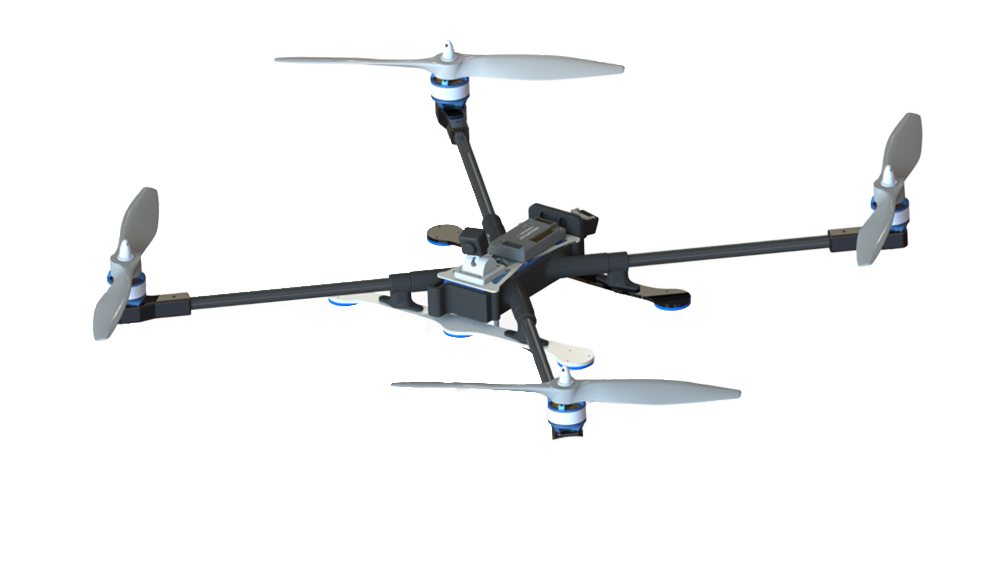
\includegraphics[scale=0.65]{figure/KestrelEDS-Quadcopter_4.png}};
			
			%Omage values (propellers angular velocities)
			\draw[-latex] (-2.05,0.575) arc (55:-15:0.35cm);
			\draw[latex-] (-0.1,1.625) arc (-25:-120:0.30cm);
			\draw[-latex] (2.17,0.97) arc (55:-15:0.35cm);
			\draw[latex-] (0.6225,-0.1725) arc (-25:-120:0.30cm);
			
			%Froce vectors
			\draw[-latex] (-2.065,0.25) coordinate -- (-2.065,0.75) node[left]{$\Omega_1$};
			\draw[-latex] (-0.29,1.35) coordinate -- (-0.29,1.85) node[left]{$\Omega_2$};
			\draw[-latex] (2.135,0.675) coordinate -- (2.135,1.175) node[right]{$\Omega_3$};
			\draw[-latex] (0.36,-0.45) coordinate -- (0.36,0.05) coordinate;
			\draw (0.85,-0.5225) node[above]{$\Omega_4$};
			
			%Inertial reference system
			\draw[-latex] (-3.05,-3.5) coordinate -- (-3.05,-2) coordinate node[anchor=east]{$Z$};
			\draw[-latex] (-3.05,-3.5) coordinate -- (-4.05,-3.7125) coordinate node[above 
			left]{$X$};
			\draw[-latex] (-3.05,-3.5) coordinate -- (-2.25,-3.725) coordinate node[below 
			left]{$Y$};
			\draw (-3.05,-3.4) node[right]{$O_{FI}$};
			
			\end{tikzpicture}
		}
	\end{center}
\end{figure}

\end{document}